%--------|---------|---------|---------|---------|---------|---------|---------|
%       10        20        30        40        50        60        70        80
%===============================================================================



% Return of Uchly Namen was the first campaign I wrote for what has now become
% hactac rule set and world setting. It is intended to be an intro start for
% a handful of newbie characters, fresh out of the Dungeon of Testing.


% TODO: update to dap
% It's not updated properly to current rule set. I'll do that if/when I have
% the time. The current campaign "Goblin Destiny" has time priority.

% note, ed 180208: mostly updated to DAP ...

% this means it's written for an older rule set version.
% Mainly: "capacity" should be replaced with "action points"
% capacity 1-9 should be 3ap base
% capacity 10-12 is 4ap
% capacity 13-15 is 5ap.
% most goblin npcs should have 4-5ap, orcs should have 3-4ap base
% then add the "quick" level to the base ap:
% base ap 4, quick 2 :  ap 6(4)

% It was played with maptool 1.2.
% I'll see if I can package the maps, images, and maptool campaign files later.





%===============================================================================

\documentclass[11pt, twoside, titlepage, a4paper]{report}

%% for xelatex and fontspec for searchable ligatures in pdf:
%\usepackage{fontspec}        % searchable ligatures in pdf
%% utf8 inputenc is ignored for xelatex utf8 based default

% for pdflatex, faster older, ligatures break search in pdf:   << fix with cmap
\usepackage{mmap}    % add letter sequences to pdf info for searchable ligatures
\usepackage[T1]{fontenc}    % ligatures break search in pdf    << fix with cmap
% set utf8 encoding, and set font encoding T1 to allow "|" ">" "<" etc
\usepackage[utf8]{inputenc}

\usepackage[a4paper,inner=40mm,outer=25mm,top=25mm,bottom=25mm,pdftex]{geometry}
% These page settings give images 1.0\linewidth around 135-140mm wide (ca 138mm)
% meaning a 300dpi image is around 1600 pixels wide
\usepackage{graphicx}   % For eps figures
\usepackage{epsfig}     % Alternative package
\usepackage[hang,small,bf]{caption}

\usepackage[british]{babel}       

\usepackage[yyyymmdd]{datetime}
\renewcommand{\dateseparator}{--}

\usepackage{fancyhdr}
\pagestyle{fancy}
% with this we ensure that the chapter and section
% headings are in lowercase.
\renewcommand{\chaptermark}[1]{\markboth{#1}{}}
\renewcommand{\sectionmark}[1]{\markright{\thesection\ #1}}
\fancyhf{} % delete current setting for header and footer
\fancyhead[LE,RO]{\bfseries\thepage}
\fancyhead[LO]{\bfseries\rightmark}
\fancyhead[RE]{\bfseries\leftmark}
\renewcommand{\headrulewidth}{0.5pt}
\renewcommand{\footrulewidth}{0pt}
\addtolength{\headheight}{0.5pt} % make space for the rule
\fancypagestyle{plain}{%
    \fancyhead{} % get rid of headers on plain pages
    \renewcommand{\headrulewidth}{0pt} % and the line
}


% remove forced implicit vertical whitespace before and after verbatim environment
\makeatletter
\preto{\@verbatim}{\topsep=0pt \partopsep=0pt }
\makeatother


% allow to force indentation of first line in section
% \indent is not working, so workaround \hspace{\parindent} works
\newcommand{\forceindent}{\hspace{\parindent}}


\newcommand{\degrees}{$^\circ$~}
\newcommand{\degree}{$^\circ$}
\newcommand{\ca}{$\approx$}

\newcommand{\vs}{$\backslash\ $}  % "versus" slash
\newcommand{\bs}{$\backslash\ $}  % just backslash


% want clear dash insert commands
\newcommand{\dash}{-}     % just a normal hyphen dash  "-"
\newcommand{\ndash}{--}   % n-dash "--"
\newcommand{\mdash}{---}  % m-dash "---"


%link new command names to the original font sizes,
%for easier to remember smaller font size
\newcommand{\vsmall}{\footnotesize}  % simpler to remember
\newcommand{\vvsmall}{\scriptsize}   %
%\newcommand{\vvvsmall}{\tiny}


\usepackage[colorlinks=true,linkcolor=black,urlcolor=blue]{hyperref}


\usepackage{ifthen}


% \needspace{5\baselineskip}      << reserves approximately 5 lines, leaves raggedbottom, more efficient
% \Needspace{5\baselineskip}      << reserves exactly 5 lines, leaves raggedbottom, less efficient
% \Needpsace*{5\baselineskip}     << leaves flushbottom if \flushbottom is in effect, otherwise ragged
\usepackage{needspace}



% \skill{blabla}
\newboolean{skillsaslist}
\setboolean{skillsaslist}{true}
\ifthenelse{\boolean{skillsaslist}}{\newcommand{\skill}[1]{\item[#1]}}{\newcommand{\skill}[1]{\subsubsection*{#1}}}
\ifthenelse{\boolean{skillsaslist}}{\newcommand{\openskillslist}{\begin{description}}}{\newcommand{\openskillslist}{}}
\ifthenelse{\boolean{skillsaslist}}{\newcommand{\closeskillslist}{\end{description}}}{\newcommand{\closeskillslist}{}}

% \action{blabla}
\newboolean{actionsaslist}
\setboolean{actionsaslist}{true}
\ifthenelse{\boolean{actionsaslist}}{\newcommand{\action}[1]{\item[#1]}}{\newcommand{\action}[1]{\subsubsection*{#1}}}
\ifthenelse{\boolean{actionsaslist}}{\newcommand{\openactionslist}{\begin{description}}}{\newcommand{\openactionslist}{}}
\ifthenelse{\boolean{actionsaslist}}{\newcommand{\closeactionslist}{\end{description}}}{\newcommand{\closeactionslist}{}}

% \eqitem{blabla}
\newboolean{itemsaslist}
\setboolean{itemsaslist}{true}
\ifthenelse{\boolean{itemsaslist}}{\newcommand{\eqitem}[1]{\item[#1]}}{\newcommand{\eqitem}[1]{\subsubsection*{#1}}}
\ifthenelse{\boolean{itemsaslist}}{\newcommand{\openitemslist}{\begin{description}}}{\newcommand{\openactionslist}{}}
\ifthenelse{\boolean{itemsaslist}}{\newcommand{\closeitemslist}{\end{description}}}{\newcommand{\closeactionslist}{}}


\newenvironment{readoutloud}%
{\begin{quote}\begin{itshape}}%
{\end{itshape}\end{quote}}%



% need a nice easily visible TODO marker
\newcommand{\todo}{\textbf{TODO:}~}
\newcommand{\TODO}{\LARGE\textbf{TODO:}\normalsize~}




\begin{document}


%-------------------------------------------------------------------------------
% make a simple title page
%-------------------------

\begin{titlepage}

\begin{center}

   \vspace{4 cm}

   \textbf{\Huge{Return of}}

   \

   \textbf{\Huge{Uchly Namen}}

   \

   \textbf{\Large{newbie introduction campaign}}

   \vspace{2 cm}
   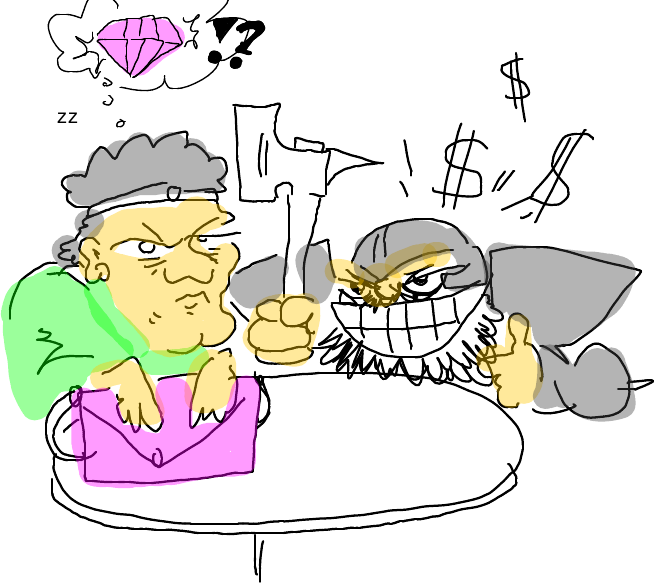
\includegraphics[width=120mm]{./figs/playthrough/negotiate.png}

   % make it look better in html rendering.
   \vspace{2 cm}

   \normalsize
   four main adventures, plus side quests\\
   ca 50h game time


   \vfill % Puts what's below at the bottom of the page

   %\textbf{\Large{Author Authorson}} %\hspace{5 cm} \large{author2}}

   \

   %\large{company name}

   %\large{General Academy of Bloody Murder}

   \

   \normalsize{\today}

\end{center}

%\thispagestyle{empty} % No page number on title page.

\end{titlepage}




%-------------------------------------------------------------------------------
% copyright etc on the back side of the title page
%-------------------------------------------------

\raggedbottom

%\vspace*{\fill}

\thispagestyle{empty} % no header on this page

\vsmall
\noindent 
This work is licensed under a Creative Commons \\
Attribution-NonCommercial-ShareAlike 4.0 \\
International License. (CC BY-NC-SA 4.0).\\
\url{https://creativecommons.org/licenses/by-nc-sa/4.0/} \\
\url{https://creativecommons.org/licenses/by-nc-sa/4.0/legalcode} \\
If you want to use it in any other fashion please contact the author.

\

\noindent
All images are temporary placeholders, \\
most are downloaded and unattributed.\\
They need to be replaced with licensed art.

\normalsize

%\vspace*{\fill}
%\vfill


% Add a table of contents
\clearpage              % don't allow anything else, above, on the TOC pages.
\flushbottom
\tableofcontents        % Always compile twice if you have changed much
\newpage                % don't allow anything else, below, on the TOC pages.



% disables chapter, section and subsection numbering
\setcounter{secnumdepth}{-1}
% This way I don't have to use chapter*{} or section*{} together with manually adding the table of contents lines, which also screws up the page headers.



















%===============================================================================
%                         here the adventure begins
%                         -------------------------


%\cleardoublepage
\clearpage
%\mainmatter  -- nope, not in article or report ?
\setcounter{page}{1}
\flushbottom
\phantomsection\addcontentsline{toc}{section}{introduction}
\section*{Introduction}
\chaptermark{introduction}
Hello, good folk. This is a simple newbie campaign from the old days. It is the first one I wrote for what has become the hactac rules and world setting. Intended as a first introductory campaign for new players and characters, to showcase some world intro, basic maps, fighting techniques, etc.

Some of the maps and token images I've found on various rpg and table top user gallery sites and shamelessly used here without proper attribution. If you find your material in here and either want me to remove it or want proper attribution, please contact me.

The campaign consists of a series of adventures linked together around the return of the demon Uchly Namen and the problems he causes. This is meant to be played as tongue-in-cheek old style gaming and is supposed to be fun and entertaining. Don't bother about realism, dark intrigue, etc. Happily portray the npc characters as cliché cardboard cut-outs, use silly voices, be flexible with the rules, and so on. Maximum fun!

\begin{readoutloud}
Text looking like this is supposed to be read to your player in true old school style. Don your best silly voice acting hat.
\end{readoutloud}

I've tried to balance the encounters to fit a group of a few 100xp newbies character, straight rolled and without serious optimisation beyond what is recommended in the campaign section of the rule book.
It is recommended that all players roll up characters and run through the \emph{Dungeon of Testing} adventure to get used to maptool and the rules. That is also a good way to find glaring tactical holes in the newly created characters.

There are plenty of opportunities where HareBrained Heroes can charge into Gory Glory and Certain Death, but there are usually less risky alternative paths to take if the players explore and assess the situation before hammering their head into the wall. If a Hero falls, have the player make a new one and let it inherit some of the xp from the previous. E.g: First Fred dies after gaining 50xp from the first few adventures. Second Sam can then be built with +30xp inherited? Discuss it with the players to balance the loss against keeping pace with the rest of the party.

If you run this campaign for a larger group, more experienced players, or better characters please adjust the opposition. The easiest way is to just increase the amount of critters, or upgrading a couple of them to more potent variants. Most maps have nooks and crannies where reinforcements or hidden reserves can be spawned without breaking the logic of the encounter. Also, if the enemies seem to be overwhelmingly difficult, just delete some of them. Encounters should be dangerous. Deadly for the careless, but manageable if the players are smart.

Before actually playing each sub-quest, try to run it through in your mind and consider some possible actions and choices your players might make, and their consequences in terms of outcome and losses. Don't be afraid to kill a character or two every now and then if they are reckless, but the players should be given reasonable warning before heading into a trap which they cannot get out of. Also, it is good to provide avenues of escape and retreat if possible, so that they can flee from enemies that turn out to be too powerful. Live and wisen up for the future.

The different sub-quests are designed to showcase different tactical issues with the hactac rule set and world. The combat power of new player groups vary quite a bit so it's likely that the encounters need to be adjusted to suit your particular group of murderers. Also, veteran tabletop players will probably be better at the early stage optimisation of their characters, which means their characters will have more combat prowess per xp than characters created by newbie players.

\

The first run through of the campaign was 2009-12-02 to 2010-05-17. It took a total of 21 weekday evening sessions, of 2-3h each for a total game time around 50h. The early sessions had some technical issues that took some time to work through, but all in all the MapTool-1.2-b32 worked quite well, as did Jarnal-917. We started out with skype for voice chat but had to switch since it was way too unreliable and problematic. Teamspeak3 worked much better, but with some minor issues regarding latency. Mumble should be a great replacement, but has not been tested yet. \emph{Note: In late 2017 we run exclusively with mumble and mostly with MapTool-1.4.0.5, with Jarnal collecting dust for quite a while.}

If I get the time I might update the campaign files to MapTool-1.3 series format, but in the mean time the 1.2-b32 release works well enough.\\

\

...

\

\emph{sometime 2015:} Well now I'm sitting here taking a deep breath and going through the files and dreading all the boring work needed to redo this as maptool version 1.3 campaign files. Blaurgh! Well, we'll just have to see if I have the stamina... or I might need a Quaff! So, it's not happening anytime soon.

\

The campaign chronology of the first run-through can be found at \\
\url{http://forums.rptools.net/viewforum.php?f=48} \\
and the discussion forum for this campaign is located at \\ \url{http://add.url.here.org/sothat/wecan/readit}

I have also reproduced it here as an appendix. The \hyperref[sec:playthrough]{"Playthrough section"} is the original posted chronology, but cleaned up.

\


%TODO: \\
%
%
%TOKENS: \\
%- Pawa civilians \\
%
%
%MAPS: \\
%-Pawa castle \\
%-Conq castle \\






%The Return of Uchly Namen
%-------------------------
\clearpage
\section*{Return of Uchly Namen}

The Baron Evilnius Conq is trying to win more power and wealth by taking over the lands and castle of Baron Massa Pawa. But he cannot do it by ordinary means. Instead he has hired the wizard Deville Sneexious.
She managed to find a way, by summoning the demon Uchly Namen to do her bidding, and let the demon break into the Pawa castle and kill the nobleman and his guard captain.

The thing is that the demon has been summoned once before, to do exactly the same thing, some 200 years ago, and between the ancestors of the Conq and Pawa lines no less: Moronius Conq, who felt he wanted to kill and supplant Lotsa Pawa, hired the wizard Trygain John to summon the demon and have it attack Castle Pawa. Trygain was a bit fumbly and did a piss poor job of the summoning and subsequent binding, as well as giving the demon very vague commands. The demon attacked the castle half-heartedly for a while, then considered itself finished with the command and went on a rampage across the region for a week or two. Back then some stalwart Heroes with the wizard Honorbliz Wize on point managed to force him back to the summoning site, and finally out and away from this realm. After the fight Honorbliz Wize took upon himself to seal the demon from this world and scatter the binding artefact, a large necklace, in four pieces.

Sneexious have located one of the pieces, the necklace itself, but is missing three gem stones. She knows approximately where they are, but have not been able to find them. The last gang she sent went missing after recovering the RedStone. The village of Sleepy Cove has few heroes, so she has had to lower her standards. And just then the stalwart group of noobs land in the harbour on a warm summer evening...

\

Sneexious is living in Sleepy Cove under the guise of a wise woman scholar, Dyslexia Marigt. An elderly lady who only does good for the fellow villagers around her. The nice old Dyslexia Marigt have dug up the horrible secret of the "Return of Uchly Namen". She will talk to the adventurers and present her plight as follows: \\
If they cannot find all three gems: RedStone, GreenStone, BlueStone, and bring them to her before the end of the summer, the Demon of Old, Uchly Namen, will rise again. As he did once before, he will lay waste to the region. This happened already some 200 years ago, and the stars are coming into alignment for it to happen again. She must rebuild the binding artefact to prevent the demon from entering this realm.

Now, if the heroes would please be so kind as to find all three gem stones and bring them to her, she will take them to the gate site to "sacrifice the binding artefact" and close the gate \emph{forever}!

In fact she will sacrifice the Heroes, or some unlucky farm girl, to open the gate and bring forth the demon, binding the beast to the command of the bearer of the necklace.
Most likely the summoning and binding will not go as planned due to the interruption of the heroes, and the demon will emerge unbound, and much more difficult to command. The demon will then start his rampage across the region.

Sneexious will then go to the Old East Tower ruin and meet lord Conq. There she will keep him in the dark about the problems with the demon, and agree to complete the assault on Castle Pawa. She will command the demon to attack, then follow Conq to his castle for the rest of her payment.

The demon will attack the Pawa castle and kill the lord and captain, and anyone else in the way. After that irritating command it wants to kill Sneexious, and heads off towards the west to find her, passing through Sleepy Cove.

Lord Conq has long been waiting for this event, and will take his small army and march into the battered Castle Pawa, to "rescue" and "protect" them from their horrible fate at the hands of the demon monster.

Sneexious has been paid, but must somehow escape both the demon and the agents and assassins she is certain that Conq has sent after her to ensure she banishes the demon, and perhaps kill and rob her anyway afterwards.

It is now up to the heroes to stop the demon from destroying Sleepy Cove. They will fight it valiantly, but it is not enough. In the end the final blow will be dealt by the obnoxious True Hero, Bling SwordSlash.

It is possible that the Heroes choose to get involved with the problems at Pawa castle, but it is unlikely they will be able to do anything useful there. They might succeed in capturing Sneexious though, but that will bring them into conflict with Conq's assassins.




\subsection*{Synopsis}
\begin{description}

\item[00] Recruitment, find Dyslexia Marigt, get the job, figure out where to start.


\item[01] Search for the goblin bandits in the south forest, kill them all, get the RedStone.


\item[02] Travel to Eisenkrafs, search for Coal-Black-George, find a way into the mine, down shaft 5-1, into the natural cavern, while getting set up by the mining boss. Find the body of Coal-Black-George and get the GreenStone. Survive to find another way out, since the boss and his gang will kill those who try to leave the way they came in.


\item[03] Travel to Honorbliz Wize tower, see the fight between the wizard and Sam Slick. Take side perhaps. Search the tower for the BlueStone, while fighting off the shadow servants. Perhaps figure out that Honorbliz helped banish the demon the first time, that the effective weapons are in Castle Pawa, and that something is wrong with Dyslexia Marigt's story.


\item[intermission] Rest and recuperate. Decide whether to continue helping Dyslexia Marigt for some more gold. Perhaps figure out that Dyslexia Marigt is planning on using human sacrifice in her "gate sealing" ritual. Also a good time to go back to Eisenkrafs to take revenge on Goebbels, clear out the bandits, etc.


\item[04] Gate site, either as unwitting sacrifices, or to save kidnapped girls. Fight the guards, and the wizard, then flee from the demon.


\item[05] The Old Eastern Tower Ruins. Meeting between Dyslexia Marigt and Baron Evilnius Conq. Figure out more of the story, and where the demon will be heading.


\item[06] Attack on Castle Pawa. perhaps they will just hear of this, not be there. If there, fight the demon, but first find the weapons. The old lance spear and shield.


\item[intermission] Demons on the Loose. A clan of Grey Stalkers have slipped in through the not quite closed gate. They waylay the Heroes for food and fun.


\item[07] The attack on Sleepy Cove. Fight the demon, then Bling SwordSlash will take over, make the killing blow, and get all the credit.

\end{description}



\subsection*{Main NPCs}

\begin{description}

\item[Deville Sneexious:] A greedy old wizard. She is not as competent as she thinks, and lazy to boot. She is however great at talking the talk and playing the part. She is hired by Baron Conq to summon Uchly Namen to attack Castle Pawa. Being a bit lazy she delegates the small stuff to the Heroes.

She lives in Sleepy Cove since winter, under the guise of "Dyslexia Marigt", a pleasant old scholarly woman who is trying to save the region from the impending doom.


\item[Bling SwordSlash:] A True Hero of many Great Deeds in far away lands. He is currently summering for a short while in Sleepy Cove. He was there since he heard Sneexious was looking for help with something about a Demon. But since she is paying a pittance for the services she asks for he mostly sits in the inn and drinks. He is enjoying most of the naive young women in the village and is in no hurry to leave.

He started believing the stories about himself a long time ago, and is sooo much better than everyone else. Simply above all the other cretins around, with the correct moral values, only charging reasonable sums of money, etc.

Bling SwordSlash will steal all the Glory and Praise from the Heroes in the conclusion of the campaign, and he should be seriously disliked before that to make the bitterness taste even worse. It should not be hard, just play on his arrogance, obnoxiousness, know-it-all-itude, and "Moral Values" preaching.


\item[Sam Slick:] A roaming cloak and dagger thief, who has caught the scent of gold and foul play in the region. There must be money to be liberated. He is ego focused, direct, and very skilled with practical flexible grey morals. That said, he can be friendly and helpful as long as it doesn't cost him anything.


\item[Honorbliz Wize:] is the old wizard who once before helped banish Uchly Namen. He will most likely make a very brief acquaintance with the Heroes before dying.


\item[Baron Evilnius Conq:] Spoken of as "The Baron" or "Baron Conq", is a sly evil man in his early 30's. He is power hungry and greedy, missing few opportunities to cook up plots and plans. However, he is not an overly bothersome tyrant to the people living on his lands. As long as they pay their taxes he will simply not bother with them at all. They are beneath him.

Instead he focuses all his energy on schemes to increase his power amongst the nobility. His next ploy is to try to take over the Pawa lands and riches. Something his great, great, ..., grandfather tried before him with little success. Evilnius, however, feels he can do better than his ancestor Moronius.


\item[RedGuard:] Conq's elite guards. They are dangerous in a fight since they can make multiple accurate attacks with their wicked sharp staffs. Other than fighting they are mostly silent and sombre.


\item[Baron Massa Pawa:] is the old, wise, honest, and well liked ruler of Castle Pawa and the surrounding lands and villages. The Heroes might seek an audience with him before the attack by Uchly Namen. Otherwise they will just hear of his death.


\item[Gebbhard Goebbels:] the mining boss in Eisenkrafs. He is the foul ruthless de facto ruler of the mining village of Eisenkrafs. Fat and 50+ he is still large and strong, and will be a problem for the Heroes unless they find a way around him and his ruffians.


\item[Uchly Namen:] A great demon from beyond. He has been called here before. The place has tasty creatures, but the wizards who strive to command him are always a serious pain in the ass. He has no intention of staying longer than he has to, as long as someone has the necklace and is using it to command him. If he can get that effing necklace ... well that would be a whole new situation indeed.

He cannot directly attack the bearer of the necklace, and must obey their commands to some extent, although the control is limited and the details up to interpretation. He can only speak Ancient and does not understand Common. After the attack at Castle Pawa he always carries around an old scholar who is forced to translate for him.

He is very powerful and too dangerous to battle without the lance spear and shield from Castle Pawa. There is no use setting numbers to this beast. He will behave according to script to make it dramatic, frustrating and fun.

\end{description}










\raggedbottom
%-------------------------------------------------------------------------------
%                             Introduction
%                             ------------


\phantomsection\addcontentsline{toc}{section}{player introduction}
\section*{Player introduction}
\chaptermark{player intro}

Open the game by showing the players the region map. Say they all come from the west to TradeTown in search for Gold and Glory! Then continue with a traditional narrator voice and read out the section below:

\begin{readoutloud}
The newbie Heroes have all arrived in Trade Town last week. They have been looking for work, but it has been difficult to get anything worthy of a true Hero wannabe.
Then suddenly they find an old advertisement proclaiming:

%\begin{center} 
%\begin{minipage}{0.6\textwidth}
\small \begin{verbatim}
Dyslexia Marigt, Scholar Supreme,
is looking for brave adventurers,
to procure special items and run
interesting errands.
Payment in gold, upon delivery!
Contact D.M. in Sleepy Cove.
\end{verbatim} \normalsize
%\end{minipage}
%\end{center}

The advertisement is tattered and worn, but it is the best thing available. The Heroes gather their meagre belongings and buy passage on a ship the very next day. After a short and sunny cruise the Heroes finally disembark on the pier of Sleepy Cove harbour, late on a beautiful summer's day.\\
The smell of adventure, heroic deeds, and gold is in the air...

\

... and it also smells a bit of fish.
\end{readoutloud}


This should get the Heroes in gear. Show them the map of Sleepy Cove and place their figure tokens on the pier. Then let them decide what to do from there. Likely they'll go into town, ask around for Dyslexia Marigt, the inn, or the store to get equipment.


\goodbreak
\begin{samepage}

\subsection*{The Region around Sleepy Cove, KingsLand}
%-----------------------------------------------------
The Heroes will spend most of the time making expeditions out of Sleepy Cove, a slow little fishing village in Baron Conq's domain, a short boat ride from Trade Town.

\begin{center}
\vspace{1 cm}
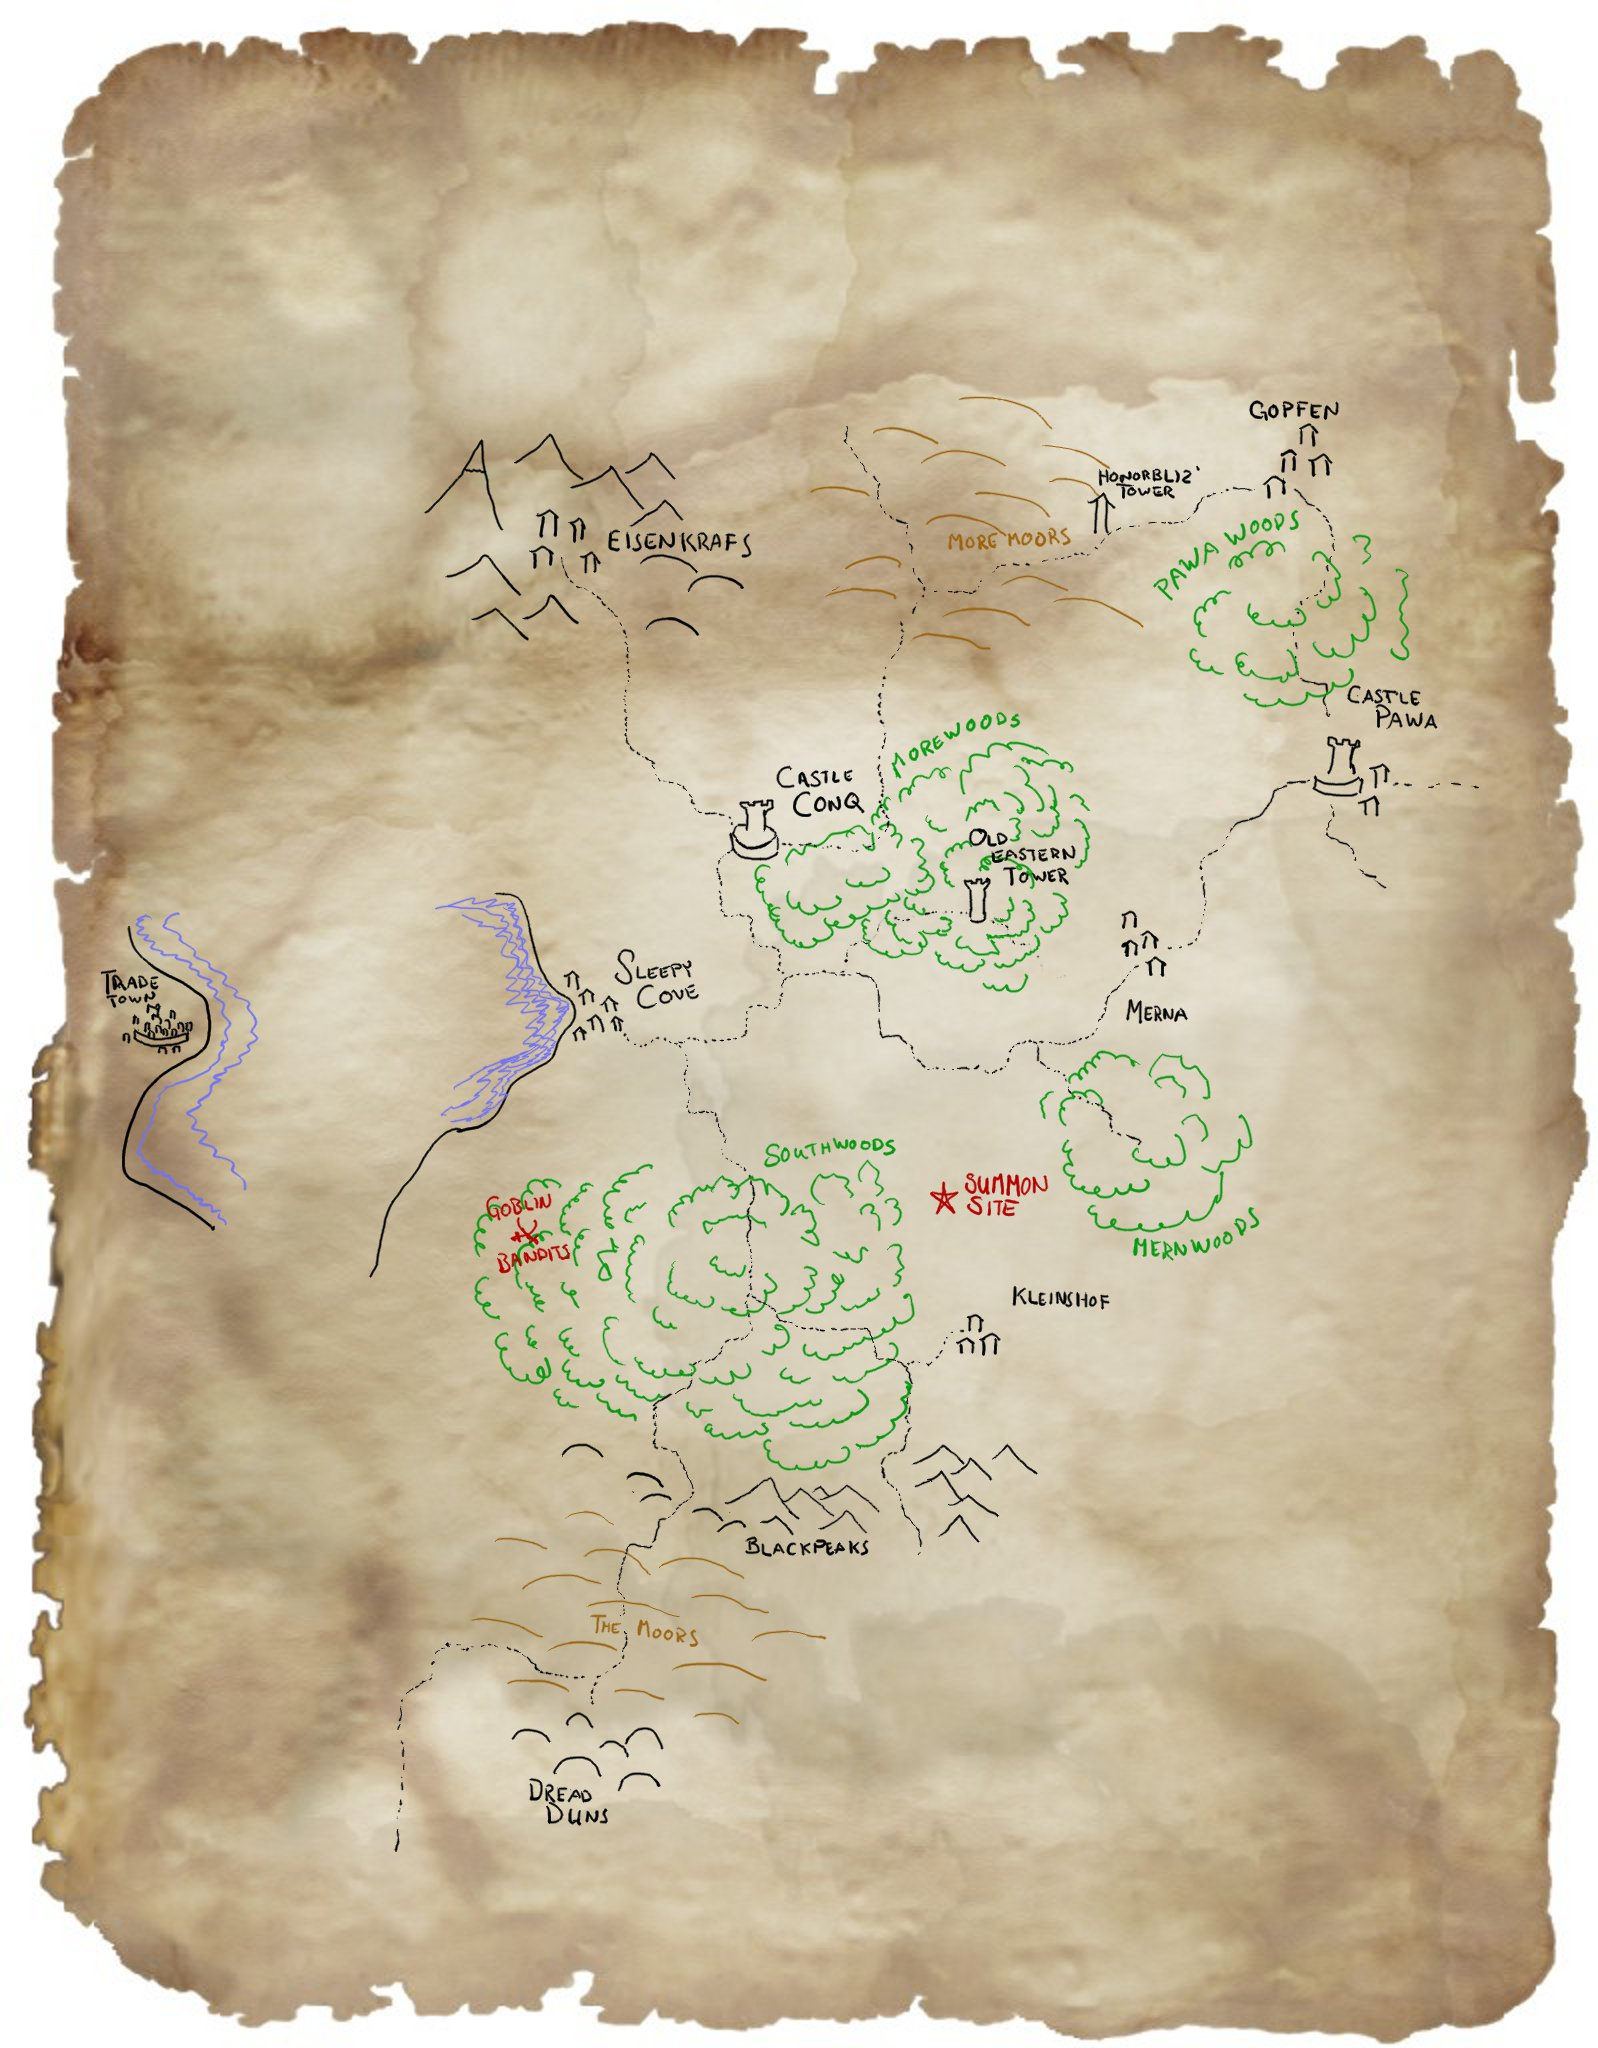
\includegraphics[width=1.0\linewidth]{./maps/region-gm.jpg}
\end{center}

\end{samepage}







%--------------------------------------------
%00 : The Recruitment - Welcome to Sleepy Cove
%===============================================================================
%                              Sleepy Cove
%                              -----------


\clearpage
\phantomsection\addcontentsline{toc}{section}{00 recruitment, Sleepy Cove}
\section*{00: The Recruitment -- Welcome to Sleepy Cove}
\chaptermark{sleepy cove}
\flushbottom

\subsection*{Synopsis}
%---------------------
The Heroes arrive at Sleepy Cove. They find their way to Dyslexia Marigt and take the job of getting the stones. They get some advice and directions to get started.


\subsection*{The Village of Sleepy Cove}
%------------------------
\begin{readoutloud}
A quaint little fishing village. The houses are somewhat askew, the docks need tending, the people look a lot like each other, and a faint lingering smell of fish is everywhere. But the sun is shining and all is good.
\end{readoutloud}

The village of Sleepy Cove, a small hamlet with a sheltered harbour. It is part of Lord Conq's domain, in the kingdom of KingsLand. It is a small village, mostly fishermen and farmers. The inn "Sleep with the Fishes" is the centre of society, and the general store has basic equipment, and a 10\% chance to have any sought after "special" item available on the shelves.


\begin{center}
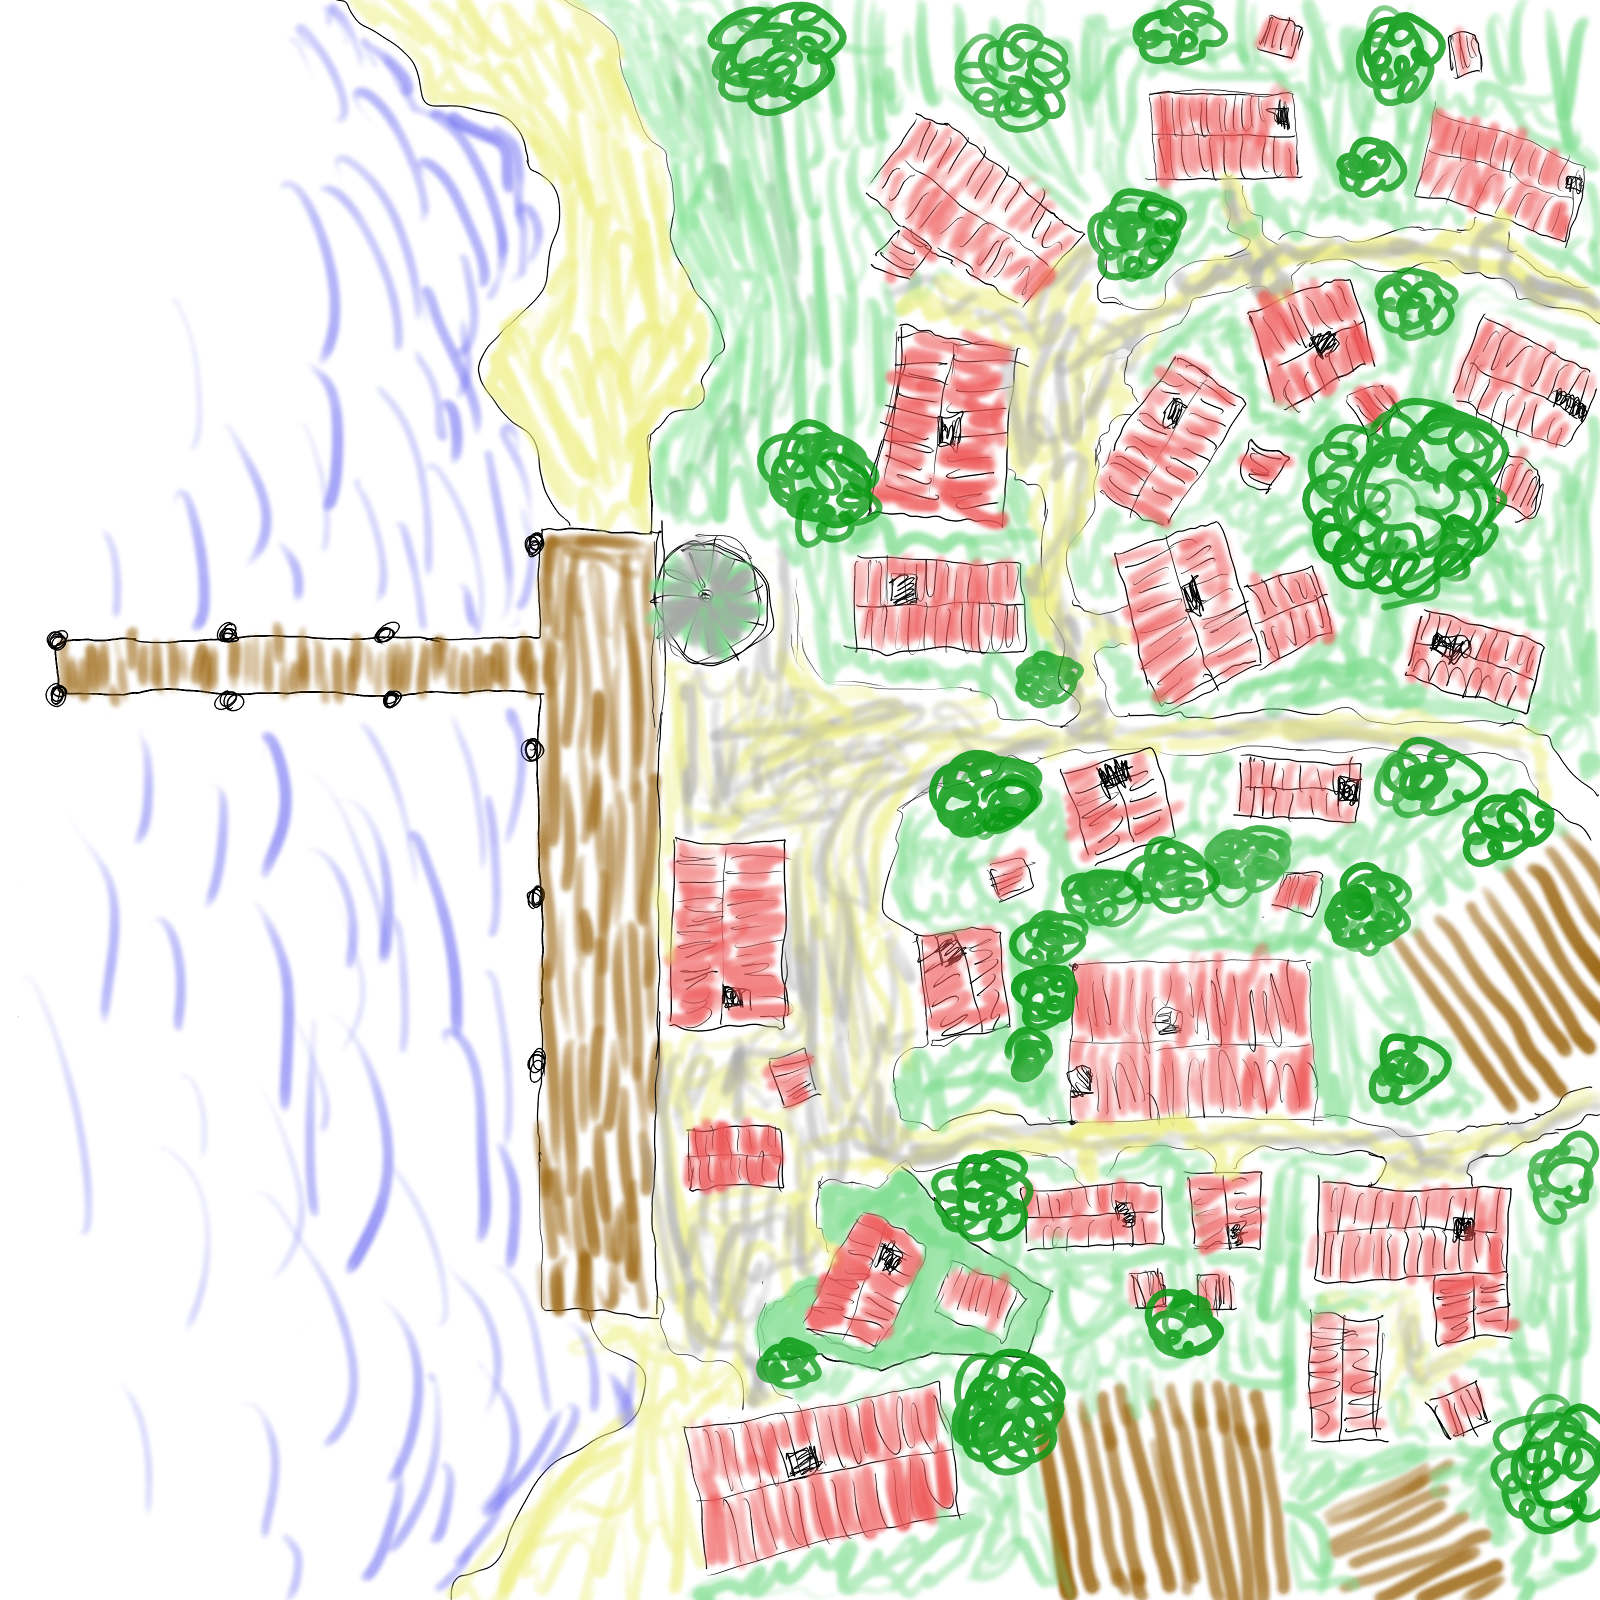
\includegraphics[width=1.0\linewidth]{./maps/Sleepy-Cove-(100x100,16+0+0).jpg}
\end{center}


\subsection*{Sleepy Cove gossip: general info}
%---------------------------------------------
Gossip success:\\
-3: There is an actual hero in the village since yesterday. Bling SwordSlash, a powerful hero of many well known deeds.  \\
+0: A scholar, Dyslexia Marigt, is looking for adventurers. \\
+0: Farmer Beard has had problems with gnabbits eating his corn. \\
+0: This is looking to be a good summer. \\
+0: This is looking to be a poor summer. \\


\subsection*{Sleepy Cove gossip: Dyslexia Marigt}
%------------------------------------------------
Gossip Success:\\
-3: Nice old lady, lives in that cottage over there...\\
-3: She is looking for a band of adventurers. \\
+0: She has been living here since midwinter. \\
+0: She always has one of Baron Conq's personal body guards with her. \\
+1: She is a bit of a loner, but quite friendly. \\
+2: She has helped diagnose and treat Brutella the Sick's illness. (random info on illness: nightdragons, elfwind, gnomethumb, greenspots, stonestomache) \\
+2: She hired a couple of adventurers about a month ago. \\
+3: The previous adventurers are said to have disappeared in the South Forest over a week ago. \\
+4: She used to work a couple of months for Baron Conq in his castle before renting a cottage here in Sleepy Cove. \\


\subsection*{Dyslexia Marigt}
%----------------------------
When entering Dyslexia's house they immediately overhear the end of a heated exchange between Dyslexia Marigt and Bling SwordSlash. They hear Bling SwordSlash say:
\begin{readoutloud}
\emph{Bling [raised voice, angry]:} Real Heroes don't work for pocket change.
\end{readoutloud}
Then he storms out, stops by the heroes and makes a derogatory stare and pff sound, and says:
\begin{readoutloud}
\emph{Bling [scornful voice]:} Well, maybe these wannabes do. Good luck with them, Sneexious! Or maybe your Conq guards can do it for free, ha? \\
Maw-Ha-ha-ha!
\end{readoutloud}

Bling knows of Deville Sneexious, and is not fooled by her alter ego disguise. He leaves the house laughing.
Dyslexia Marigt looks real angry for a second, but composes herself fast. She looks at the heroes and smiles:

\begin{readoutloud}
\emph{Dyslexia [kind old voice]:} Welcome strangers. Are you here for work? Come on in, please. I have some milk and cookies somewhere.

There is a horrible danger threatening this region. An old lingering evil since the days of yore. The Demon "Uchly Namen" will return to wreak havoc and mayhem for leagues around if we cannot stop his arrival.

The Demon Beast has been here before, some 200 years ago, but was defeated and banished forever, or so they thought. Now, the stars are coming into alignment again, allowing the monster to once again open the gate.

You see, I have learned how to block his passage into this realm, forever sealing the gate that was once left ajar after his last banishment.

I don't expect you to perform such a dangerous task. I plan to seal the gate myself. But I need a few items to do it. Three crystal stones in fact.

I'll pay 5 gold for each of the stones, and I'll double that once I have all three.

I found out about the demon when I worked for the Baron Conq a few months ago. I was hired to organise and update his family library and chronicles. There was a mention of a horrendous event some 200 years ago. I have since found, through long and painstaking research, that it was the arrival of a powerful Demon, "Uchly Namen", that caused the chaos. Unfortunately the information is a bit uncertain and incomplete in places. But I believe I've found a way to, once and for all, seal the gate through which the demon enters this world.

I have an artefact, which, when complete, can be used to seal the gate forever. Will you please help me acquire the three missing crystals?

The first, the RedStone, has been stolen by some goblin bandits, I believe.
It was over a month since I sent out the request for heroes and I already hired a couple a few weeks ago. They set out towards the Dread Duns of Doom, south of the moors, but have since vanished. I heard a rumour that they had been sighted moving north over the moors, in good health. That was about a week ago.

There is a small band of cowardly goblins in the South Forest, and I believe they have killed your predecessors, and have the RedStone now.

The second, the GreenStone, is in Eisenkrafs. A miner named Coal-Black-George has offered to sell it to me. He was supposed to travel to Sleepy Cove during the summer, but I haven't heard from him in over a month. You'll have to travel up there and get it.

The third, the BlueStone, is in the claws of a villainous old sorcerer, Ho-Bliz Wayze, who lives in the old dark and decrepit tower of his evil ancestors, on the border of Baron Pawa's domain. He has refused to sell me the stone, even if I have offered a fair price for it. I even told him of it's importance, and he still will not see reason and sell it to me.

Please go to him and persuade him to part with it. I'll give you three gold to pay him. That is more than fair for the stone. It is worth at most a few silver. It is just a common crystal after all, not a true gem.

I'll pay you for each stone when you bring them to me, and double the payment once I have all three. That is 5 gold per stone plus 15 when I have all of them. Agreed?
\end{readoutloud}


Now, will the heroes agree to this? 5+5+5+15 gold is a lot of money, and with possibilities for extra loot. This is more money than they have ever had in their life before.
Of course they can always haggle for it, but then they might end up with less.


\begin{readoutloud}
You can buy supplies in the General Store if you need anything. The store also sells a map of the region. Although finding the south forest is not that hard, just follow the road south.

If you do not have any skill in tracking, I suggest you hire yourselves a guide, or it will be difficult to find the bandits. You might be able to hire John AllBeard for a couple of coppers per day, as long as you don't expect him to do any fighting. If he has to pick up his axe he will charge a lot.
\end{readoutloud}


Evilnius Conq has set a RedGuard to protect, and control, Sneexious. She presents him as her body guard here on the outskirts of civilisation. A sombre, proper, silent, and intimidating soldier.


Bling SwordSlash will be in the "Sleep with the Fishes" most of the campaign after leaving Dyslexia Marigt. He is very full of himself and likes the eager attention of all the naive girls in the village. They even look so much alike that he can't bother to tell them apart. A whole village full of multiplets.


\subsection*{The General Store}
%------------------------------
Being the only source of commerce in the village, the store charges 20-33\% above list price on just about everything to anyone who doesn't have "haggle". But even one point of haggle will be enough to get the regular list price. They have most of the simple basic equipment, but only a 10\% chance of carrying anything special, and nothing exotic.
They will purchase second hand equipment at very low rates. Good gear at most 50\% value, goblin stuff at around 10\% value, if at all.


\subsection*{The "Sleep with the Fishes" inn}
%--------------------------------------------
This is the social centre of the village. There are almost always some people here, and it is a great place to do some gossiping to find out what is going on.

After the first day, Bling SwordSlash will be in the inn most of the time, usually surrounded by a flock of village girls.

Singalot the Bard is in the room in the evenings, entertaining the people by story after story after ballad after song about all the Great Deeds that Bling SwordSlash has done in the far off lands. Singalot is a clever bard and strokes Bling's ego, after which a slightly drunk Bling tips generously.
It is obvious that Bling's heroics are way off, and leaves a wide wake of destruction:
He cleaves the horse in two when the farmers argue about it. He kills a whole family to drive out a werewolf: "Just to be safe!". He burns the food store in the middle of the winter in order to kill an Ice Murkler which had been terrorising the village. He kills both sisters when he can't be certain about which one is the evil twin.



\raggedbottom

\goodbreak \begin{samepage} \vsmall \begin{verbatim}
===================================
RedGuard                    (named)
-----------------------------------
str  8    hp 25(18) abs 4 (plate + RedGuard ward rune tattoo)
dex  8(9) m2 w4 r7(8,7) d10(12,10)
con  7    stamina 12(10)
int  4    vision 25 160deg
psy  5    mana 10
per  6    ap 7(4)
cha  4    xp -- ( ca 400-ish )
----------
quick       3
mobile      2
focus       2
overextend  2
balance     3
quick draw  6
consistent  2
avoid       8 yield+4
brawl       7
sharpstaff 12
whirlwind   7
shield      6
sharpstaff  x
poke        x
swing       x
resilient   7
enduring    2
fast        2
----------
Ward Rune tattoo: draw 1 mana to absorb 1hp from an incoming strike.
                Automatic until mana reaches 0, does not over draw.

Quaff 2x        restore 4hp and 4sta in one round, readied quick draw from belt

sharpstaff   12 dam 6/7, penetrating 1, abs 15, parry+0/+1,
(1h/2h)         reach 1 mod-3, finesse-6
                str 7/6 (max +1 damage str bonus, max +1 penetrating str bonus)
                2h: fast+1 with str 8 and dex 8
                poke: mod-0 dam 4/5 pen 3
                swing: mod-0 slow-1 dam 8/9 pen 0

heavy RedGuard  abs 3, (less mods than normal plate armour)
brigandine      dex-1 yield bonus -0
                run-1, dash-2
                str 7 (str penalties affect all actions)
                vision-10%, cone vision max 270 deg
                acrobatics mod-3
                spellcasting mod-1
                sneak mod-2

===================================
Imposing soldier in a strange red plate armour and cloak.
Armed with a large staff with evil looking metal points in each end.
He sure looks like he knows how to fight.
\end{verbatim} \normalsize \end{samepage}

\

%TODO: write invisibility spell for her
\goodbreak \begin{samepage} \vsmall \begin{verbatim}
===================================
Dyslexia Marigt / Deville Sneexious             (named)
-----------------------------------
str  3      hp 9 abs 0 (+5 once)
dex  5      m1 w3 r5 d7
con  4      stamina 6
int  8      vision 16
psy  10(8)  mana 21(17)
per  7      ap 4
cha  7      xp --
----------
staff         3
avoid         3 yield+2
common       11
ancient       6
dwarfish      4
literate      5
counting      5
magic         6
power casting 3
powerful      4
haggle        8
----------
black bolt   9 cast 1r 1m, dam 6 +2/m, range 10 +5/m, long -3dam, penetrating
               int 7, psy 7
fire storm   6 cast 1r 1m, dam 5 +2/m, range self, radius 1 +1/m,
               duration 3r +3/m, damage each round,
               caster is immune to fire for the duration
               int 6, psy 8
slow         8 cast 1r 1m, +1target/2m, range 15 +5/m, duration 5r +2/m
               target cannot move faster than maneuver,
               and any movement gives a mod-3 penalty,
               and all actions are slow-2, i.e. pushing mod-2 more to ams.
               continue slow on psy \vs psy +2/m each round (mana paid once
               on cast) up to the max duration.
               int 4, psy 3
paralyse     6 cast 2r 2m, +1target/2m, range 10 +5/m, duration 2r +1/m
               Target cannot move or take actions that require movement.
               Continue paralyse on psy vs psy +2/m each round (mana paid once
               on cast).
               int 7, psy 9
earthling    8 cast 2r 4m, activation range contact, duration 5r +5/m,
               power +3/m
               Gives the target the ability to walk through solid objects
               at a maximum movement speed of maneuver.
               The target must pass a careful psy+power roll each round or
               bounce back to where he started, taking 1d4 damage penetrating.
               int 5, psy 6
----------
power circlet (psy+2)
armour rune amulet (armour+5) for 20r when activated (single use)
walking staff 3 dam 3 abs 6 parry+1
mana potion  restore 4 mana immediately
healing potion heal 3hp 1/r
fine robe
money ( g s c)
===================================
A small old woman with tidy grey hair and a bit too much make-up.
She is dressed in a fine robe and has a golden circlet on her head.
\end{verbatim} \normalsize \end{samepage}

\

\goodbreak \begin{samepage} \vsmall \begin{verbatim}
===================================
Bling SwordSlash            (named)
-----------------------------------
str  9(7)    hp 26(18) abs 2
dex  11(9)   m2 w4 r8 d12
con  8(7)    stamina 18(9)
int  4       vision    (set human good)
psy  8       mana 15
per  8       ap 9(4)
cha  9       xp -- (ca 1000)
----------
strong 2
agile 2
tough 1
resilient 8
enduring 9
veteran 6
quick 5
mobile 5
rapid 6
balance 4
famous 8
slugger 2

sword 16
fancy attacks 8
whirlwind 8
poke
swing

captain cardio
energizer bunny
black knight 2
Über
----------
spells
----------
equipment
money ( g s c)
===================================
legendary longsword: "slash"  mod+1 dam 13(11) abs 30 finesse 8, str 7
fashionable exquisite brigandine armour abs 2 (behaves as leather), or,
legendary plate mail abs 3 (behaves as brigandine)
\end{verbatim} \normalsize \end{samepage}

A well known hero. You have heard many songs about his heroic deeds.
Dressed in fine garments. Blond flowing hair, white glinting teeth.
Armed with his legendary long sword "Slash", he fights one handed.

Bling is too cool for stats, and I'm lazy. He has around 1000xp
and a couple of super abilities, like Über, and a lot of powerful
fighting skills and maneuvers.


\

\flushbottom

























%--------------------------------------
%01 : The RedStone - The Goblin Bandits
%===============================================================================
%                         The camp of the Goblin Bandits
%                         ------------------------------


\clearpage
\phantomsection\addcontentsline{toc}{section}{01 red stone}
\section*{01: The RedStone -- The Goblin Bandits}
\chaptermark{red stone}


\subsection*{Synopsis}
%---------------------
The Heroes will hopefully ask around in Sleepy Cove before setting out to find the Goblin Bandits. The camp is found in the west parts of the South Woods. The heroes will slay the Goblins, or some might run away. In the cave they will find the bodies of Dyslexia's earlier hirelings. Searching the cave they will find the RedStone.


\subsection*{First piece, the RedStone}
%--------------------------------------
The RedStone has been taken by goblins. Dyslexia's previous hirelings, a couple of adventurers, went to the Dread Duns of Doom in the south to retrieve the RedStone, and were spotted traversing the moors northward a few days later alive and well. Then disappeared passing through the South Woods.
The adventurers are now rotting in the eastern section of the goblin bandits' cave. Hidden in the woman's skirt, in a secret pocket is the RedStone. Or let it be found amongst the goblins' treasure.


\subsection*{Sleepy Cove gossip: About the goblin bandits}
%---------------------------------------------------------
Gossip success:\\
+0: The goblin boss and his band of goblins bandits have been seen in the south forest and roads. \\
+0: The have ambushed a couple of travellers and stolen their valuables. \\
+1: They are a greedy and cowardly bunch. \\
+2: They are about 10 goblins in the band. \\
+2: The boss is large and strong. \\
+3: They fight mainly with bows and spears. \\
+3: The boss has a magic spear that can turn enemies into frogs. \\
+6: Their lair is in the north west part of the SouthWoods \\


\subsection*{The camp site}
%--------------------------

\begin{readoutloud}
This is an open area of the forest, but the faint stench of goblins and wood smoke is drifting between the trees. Listening, you can make out faint gibberish and occasional yells further north east.
\end{readoutloud}

The goblin bandits are resting around their fire when the heroes enter the map from the south west. The goblins are unaware and relaxed and will not notice the approaching heroes unless they are careless and stand in plain view. Sneaking from tree to bush they can get close.

\begin{readoutloud}
The Goblin Bandits are sitting around a camp fire, chattering in svartlingo. They seem relaxed, but have weapons close at hand.
[per]: One is gnawing on what looks like a human hand.
\end{readoutloud}

It is possible to actually talk with the goblins instead of just killing them. They have not found the RedStone on the corpse, but they can search them and will sell the RedStone for 1g. The difficulty is getting through the first few moments peacefully, as the Heroes show up in the camp. They goblins will likely just see them as potential food. A truly impressive or scary Hero might give them pause.

Once the heroes are noticed the alarm goes and the leader MuchKlajn GoBoss starts yelling \emph{(unless a peaceful opening is reached quickly)}:

\begin{readoutloud}
\emph{GoBoss [tiny angry voice]:} Ijm MuchKlajn GoBoss. Dissis mayn Kamp. Killem ogly Hoomans!
\end{readoutloud}

Wounded or breaking goblins will flee into their cave to wake their sleeping comrades and make their stand. They will release their pet wolf and goad it to attack the heroes when they enter the cave.

Otherwise the goblins will retreat and use their archers as much as possible. Their archers will mainly go into hiding and shoot from cover, giving anyone shooting at them a mod-3 for target in cover.
This can be a frustrating fight if the goblins run around a lot and the Heroes are too slow or lacking stamina.

\begin{center}
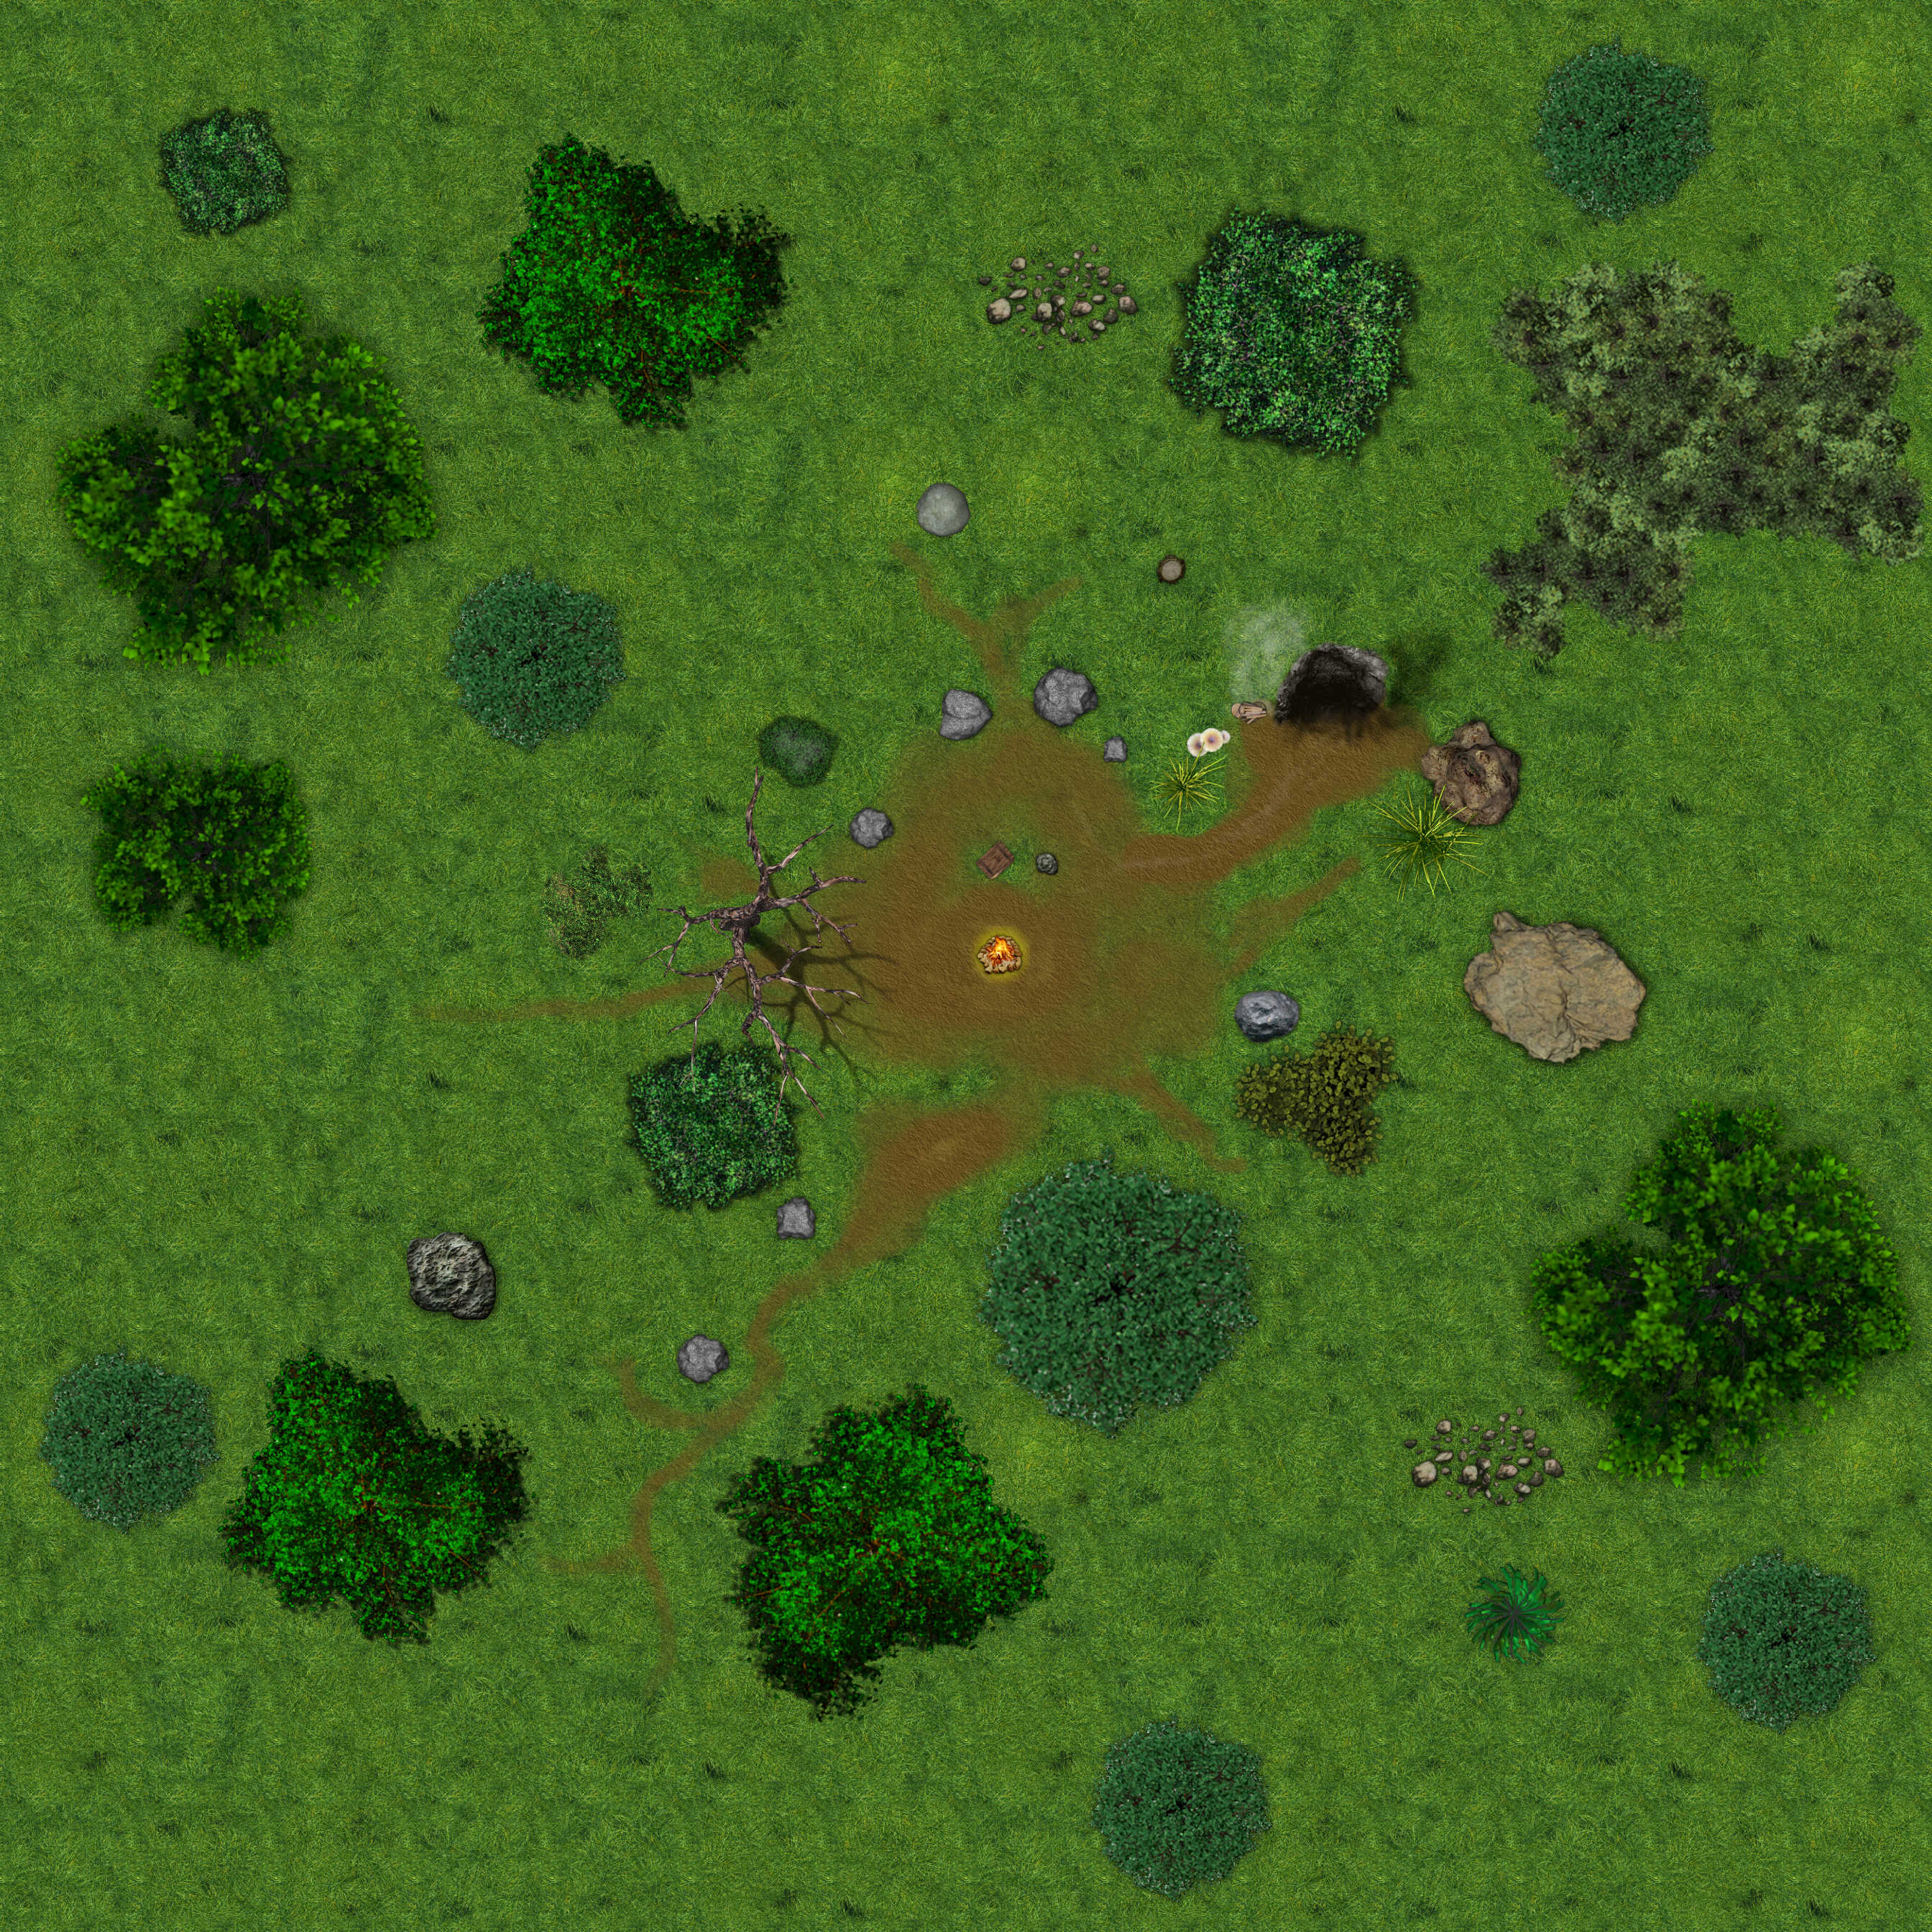
\includegraphics[width=1.0\linewidth]{./maps/goblin-camp-(32+0+0).jpg}
\end{center}

\

%\vfill



\subsection*{The cave}
%---------------------
Adjust the reinforcements in the cave to suit the situation and make an interesting fight.

\begin{readoutloud}
A dark foul smelling cave descend into the ground. The stench is horrible and almost overpowering.
\end{readoutloud}

Roll con+3 to not throw up.

The goblin cave is a dark smelly place.
The goblins will retreat to the left in the cave, wake their sleeping friends and make an ambush. The first wounded will flee further in to free the wolf. Freeing the wolf takes one round. Then they charge behind the wolf. If it doesn't go well they will try to flee out of the cave and disappear into the woods.

The treasure trove, furthest in, north of the wolf, is worth about 5 gold in all, including the coin, and requires carrying about 50 items at 20enc back to Sleepy Cove to sell it.

Let the RedStone be found either among the treasure or hidden away in a secret pocket in the dress of the dead adventurers.

\begin{center}
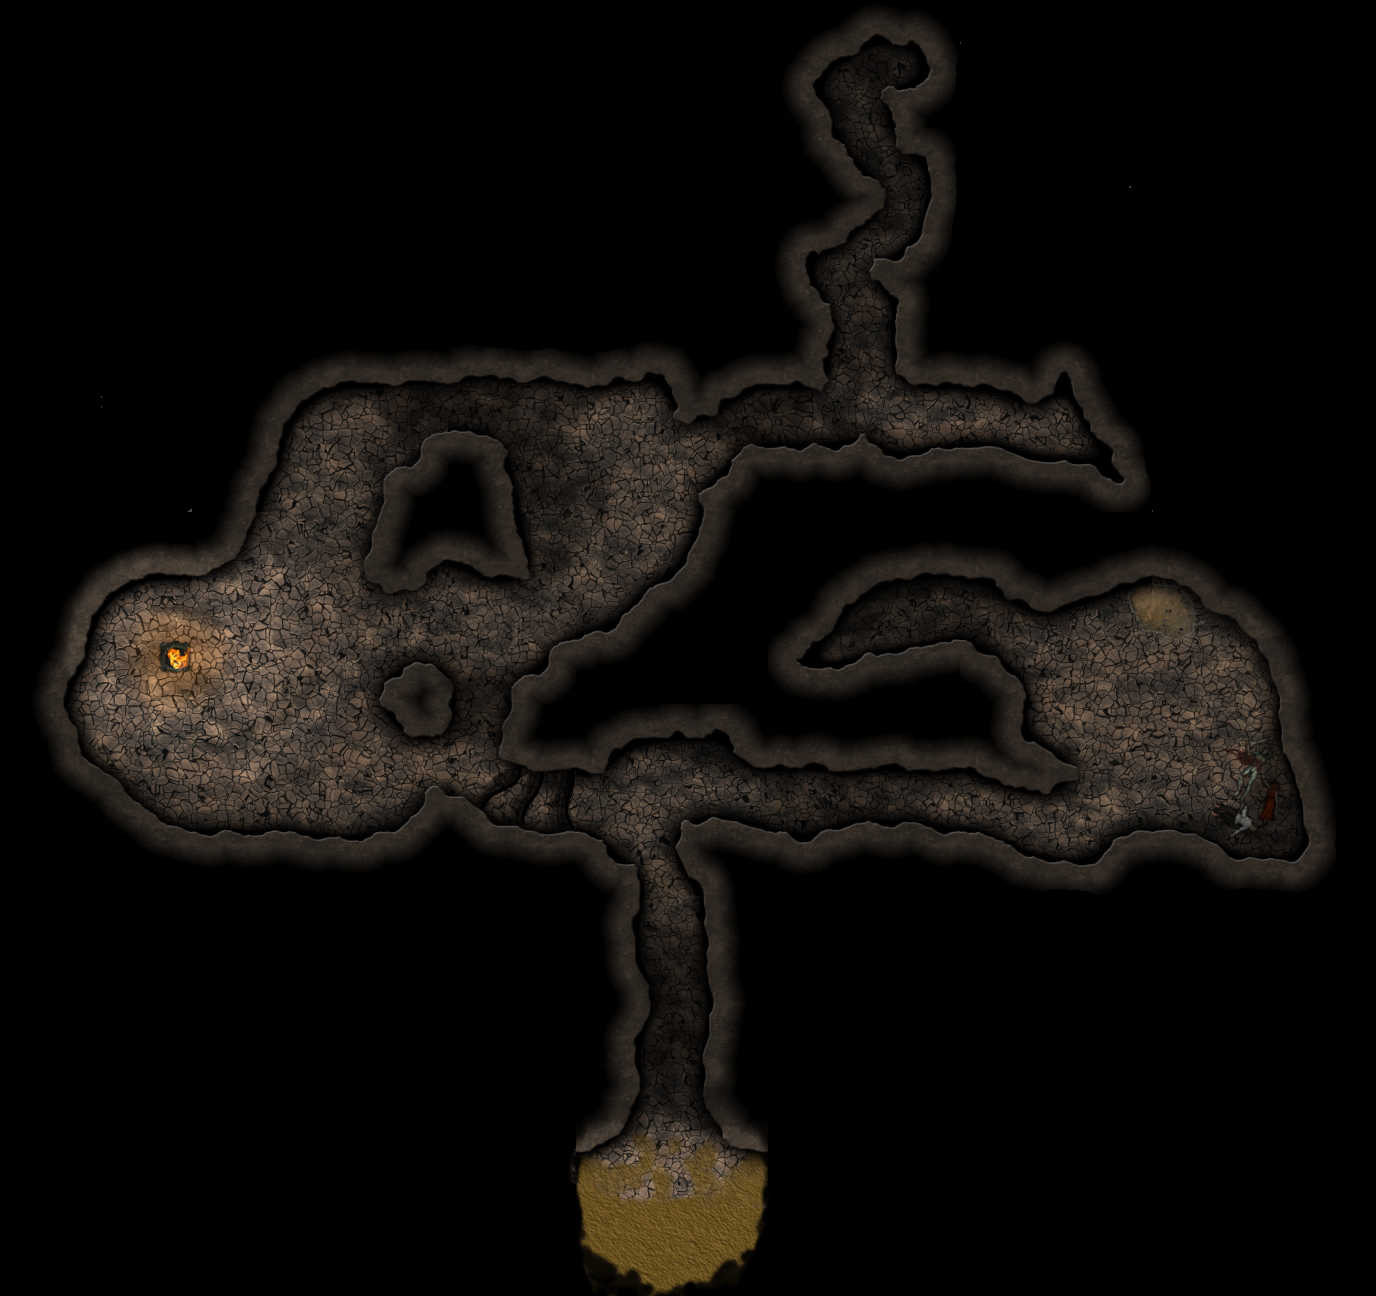
\includegraphics[width=1.0\linewidth]{./maps/goblin-cave-(32+0+0).jpg}
\end{center}

\

%\vfill


\subsection*{Opposition}
This is probably the first group fight the newly minted Heroes have gotten themselves into. Finding a good balance for the opposition is not trivial.

Start out slightly low in the camp and see how well it goes. You can bring in some reinforcement from the cave.
Then, as they progress into the cave, you balance the number and composition on how well the Heroes did in the camp, and their hp and mana status.

For three reasonably well built newbie Heroes the following should be suitable to start off the fight in the camp:\\
3x goblin bandits with spears\\
2x goblin bandits with clubs and shields\\
3x goblin bandits with short bows and knives\\
Then you can judge how well that went and adjust the remaining forces in the cave. The wolf

Remember that goblins are generally cowardly. They fight viciously when they clearly have the upper hand, but flee and regroup all the time when loosing. In this case they will flee into the cave after loosing about half their numbers.

Balance the camp fight for fun: reinforcements or fleeing into the cave, or both. The cave fight is the goblins' last stand, it has the boss and the wolf, and only a few will flee out and away if they can. Give the gobbos mod+6 to their break-or-hold psy rolls when fighting in the cave.


\subsection*{Aftermath}
Dyslexia Marigt will be glad and thankful when they bring back the RedStone to her. She pays the 5 gold and gives the heroes some cookies and milk.

Once the RedStone is delivered to Dyslexia Marigt each hero should get 10xp as a sub quest reward.

The heroes now have some time to rest and spend their money and xp before setting out north towards Eisenkrafs to find Coal Black George.


\subsection*{Opposition stat sheets}
%-----------------------------------

\raggedbottom

The standard goblins bandits should be taken straight from the rule book.
The most common weaponry is clubs and spears, 2h or with shields, and some with short bows and knives.

\

\goodbreak \begin{samepage} \vsmall \begin{verbatim}
The pet wolf: Graowl, a half starved poor critter
This one is weaker than the rule book standard wolves.
===================================
wolf                       (wolf02)
-----------------------------------
str  7    hp 8 abs 0
dex 10    m2 w6 r12 d20
psy  5    vision 15
per  8    initiative 12, ap 5, aggressive
----------
mobile        2
balance       3
charge        6
bite          7 dam 5
claw          5 dam 2 fast+1
avoid         4 yield+3
===================================
It takes one round to free the wolf.
\end{verbatim} \normalsize \end{samepage}

\

\goodbreak \begin{samepage} \vsmall \begin{verbatim}
Leader: MuchKlajn GoBoss
He is a slightly more powerful version of the goblin warrior.
===================================
goblin warrior           (goblin07)
-----------------------------------
str  5    hp 8 abs 1
dex  7    m1 w3 r5 d7
int  4    vision 16 dusk (set goblin good)
psy  4    ap 5(4)
per  6    initiative 10, ap5, aggressive
----------
quick          1
mobile         1
avoid          6 yield+4
sneak          8
charge         4
quickdraw      5
poke           x
swing          x
short sword    8 dam 5, abs 10,
                 str 3 (max +1 str bonus), finesse-4
                 poke: mod-1 dam-1 pen+1
                 swing: slow-1 mod-1 dam+1 todefend+2
small shield   8(6) abs 8, parry+2,
                 str 2
                 Ranged attacks mod-1 when in the way.
                 Hiding behind it (3ap) ranged mod-2
throwing knife 5 dam 2, fast+1, readied as quick draw from belt
                 range 8, short 4 mod+1, long 12 mod-3, vlong 16 mod-6 dam-1,
                 str 1 (no str bonus)
                 fast+1 if str 2 and dex 4
                 first three attacks do not require stamina
leather armour abs 1
===================================
A large fierce looking goblin dressed in a fine red silk shirt and
matching shawl, as well as leather armour.
He is armed with a short sword and small shield.
\end{verbatim} \normalsize \end{samepage}

When MuchKlajn GoBoss dies he says:
\begin{readoutloud}
    Aaargh, me Die, Like Stinky Pie.\\
    You die Too, You Stinky Shoe.\\
    You be StinkiEst of All !
\end{readoutloud}
This is his final dying curse, and the person receiving it will smell
really bad for 2d3 days before the weak magic dissipates.
The target gets the "Tasty" ability for the duration.

\flushbottom














%--------------------------------------
%02 : The GreenStone - Eisenkrafs mines
%===============================================================================
%                     Eisenkrafs mines and Coal-Black-George
%                     --------------------------------------


\clearpage
\phantomsection\addcontentsline{toc}{section}{02 green stone}
\section*{02: The GreenStone -- Eisenkrafs mines}
\chaptermark{green stone}
\label{sec:02GreenStone}


\subsection*{Synopsis}
%---------------------
The character might start out asking about Eisenkrafs before travelling there. In Eisenkrafs they ask around for Coal-Black-George. Gebbhard Goebbels contacts them and try to scare them with horror stories. When he does not succeed he will "help" them into the cave. They find the body of Coal-Black-George and the GreenStone. If they climb back out they have to battle the miner ruffians and flee or die. They can find a safe way out of the lower cave and escape with the GreenStone.


\subsection*{The second piece, the GreenStone}
%---------------------------------------------
Coal-Black-George did indeed find the GreenStone in an old abandoned mine cave in the mountains. He realised it was no valuable gem, but that it was a strangely cut crystal. So he sent word to Sleepy Cove to send message to the heralds and jewellers in Trade Town, to see if anyone had any idea of what it might be. Dyslexia sent word back that she would buy it for a gold or two, "out of historical interest". George then went into the mines for his day job, promptly fell into an old shaft and vanished. Find George's body to find the GreenStone.


\subsection*{Sleepy Cove gossip: about Eisenkrafs}
%------------------------------------------------
+0 A mining town in the north hills. \\
+0 They ship iron from our harbour sometimes. \\
+1 It is a horrible sorry place. \\
+2 There are some bandits around there. \\
+3 The mines are dangerous. \\
+4 The mine boss Grobler-something is a slimy fellow, stay clear. \\


\subsection*{Approaching Eisenkrafs village}
%-------------------------------------------
\begin{readoutloud}
The mining village of Eisenkrafs is the place where decent civilisation has gone to die, and rot, and smell really really bad. Inhabited by the desperate, the destitute, the vicious, and the foul, this village is very close to the bottom of the list of summer vacation spots. Small wood huts and hovels are crowded around a few decent houses. The place reeks of apathy and decline. Even the dark slow smoke leaving the many poorly laid chimneys has lost all hope and energy.
\end{readoutloud}


\subsection*{Eisenkrafs village}
%-------------------------------
Eisenkrafs is a horrible little mining town. It is run by Gebbhard Goebbels, foreman of the mine. It is still within the lands of Baron Evilnius Conq, and he does get some taxes from the place. Though, most tax coin disappear into the hands of Goebbels and his folks, some iron merchants in league with Goebbels, and a local bandit gang.

Purchasing food and beer can be done at the "beer house", along with some every day stuff. Equipment, etc, can be purchased from the mining yard. Prices are double the list values. Non essential stuff, not necessary for mining and surviving has only about 50\% chance of being available.


\subsection*{Coal-Black-George}
%------------------------------
The disappearance of Coal-Black-George is not that strange. He had found out that the mine boss Gebbhard Goebbels has some shady dealings with a group of bandits in the area. So Gebbhard stabbed George in the back and pushed him into a closed down mine shaft, nr 5-1.

Shaft 5-1 has been closed for years since it opens into a natural cave system which is very deep. Too dangerous to work excavation. Too many people lost to cave worms, gnobbits, lure smoke, and other problems.


\subsection*{Investigating}
%--------------------------
A good way is to start asking around in town about Coal-Black-George. Most people knew him as a good miner, "some orc and dwarf blood in those veins I'm sure." He worked hard, drank less than most, then worked even more in shut down tunnels, caves, etc.


\subsection*{Eisenkrafs gossip: general}
%---------------------------------------
+0 The mines are the only way to earn a living around here. \\
+0 There are bandits in the mountains. Stay in town, with people. \\
+1 There are bandits in the area, they are careful and sneaky, and very well informed. \\
+1 Gebbhard Goebbels is boss of the mines. Talk to him about a job. People are always missing around here. \\
+3 Gebbhard Goebbels is a shady fellow, we don't like him much.


\subsection*{Eisenkrafs gossip: about Coal-Black-George}
%-------------------------------------------------------
+0 Coal-Black-George is missing since a few weeks. \\
+1 Coal-Black-George has been eaten by the Grey Worm. \\
+1 Coal-Black-George has been killed by the bandits. \\
+1 Coal-Black-George has left for Sleepy Cove. \\
+2 Coal-Black-George went missing in the mine one day. \\
+2 Coal-Black-George had found some strange green crystal a while back. \\
+3 Coal-Black-George disappeared down shaft 5-1. What was he doing there? That shaft has been closed for years. It opens to natural caves and is too dangerous to work. \\
+6 The boss, Gebbhard Goebbels, had taken a dislike to George just before he disappeared.


\subsection*{Gebbhard Goebbels, the boss, comes to talk}
%-------------------------------------------------------
Gebbhard Goebbels will contact the Heroes once he finds out that they are asking around in town. He will say Coal-Black-George was a good fellow, but foolishly working the old tunnels. The warrens and closed down areas are swarming with horrible creatures. That it is certain death to go down there.

If he still cannot persuade the characters to give up he will offer to help set up a temporary climb. He will then set a couple of ruffians to guard the shaft for a bit and "help" the heroes get back if they locate George. He will even give them a tainted "healing potion" to give him if they find him. The potion is of course poison. Muahaha.

Gebbhard Goebbels sends two ruffians to "help the heroes down". They will help setup a long rope ladder. After the heroes have descended they will helpfully remove the ladder so that they must climb up the hard way.

This will take be 5 successful climb+3 rolls. If they have rope it is climb+6 rolls, and with proper climbing gear it is climb+9.


\subsection*{Below Shaft 5-1 : The Natural Cave}
%-----------------------------------------------
\begin{readoutloud}
As the last of you steps off the rope ladder leading up through shaft 5-1 you hear a rustling from above the shaft. All of a sudden the ladder is falling down, coiling around your feet. A few seconds later the way up and out is nothing but a large pile of rope and sticks, and the weak lantern light coming down from above dims and disappears.

\verb|--- ALTERNATIVE --- raising elevator or rope ladder:|

The last of you step off the ladder, looking into the darkness wondering what horrors will be coming to gnaw on your bones if you die here. A rustling behind you turns out the be the ladder disappearing up and away. A few seconds later the way up and out is nothing but the rough bare rock sides of shaft 5-1. The weak lantern light coming down from above then dims and disappears.
\end{readoutloud}

The cave beneath the shaft is populated with all sorts of strange cave critters.
This is a showcase of some basic cave critters, and cave fighting.

Make clear to the players after a while that there is fresh air circulating through some parts of the cave, i.e: there is at least two natural exits from the cave. This provides alternative exit possibilities to climbing up and fighting with the miner ruffians.

The east exit is blocked by rubble. Had they brought mining equipment (they didn't did they?) it would be possible to break out that way in about a day's work. Without mining equipment it will be impossible, and they must find another way. If for some bizarre reason they actually thought to bring some mining gear, just reward them with a day's digging and some ambushes by bugs, spiders or whatnot.

The south east exit is an open crawlspace, and opens into a natural old water run off, which leads for a km or two before exiting the mountain side a couple of km from Eisenkrafs. This is the easy way out.

Climbing back up is not that difficult, mod+3. Roll 5 successful climb without falling down. This is made easier if they bring climbing gear to fasten safety rope, or they can improvise with daggers and rope.

If the heroes manage to get back up from the cavern, they will probably know that George was murdered, since there is a knife sticking out of his back. They might even have a suspicion of foul play from Gebbhard Goebbels and his ruffians since the ladder was helpfully removed.

Gebbhard Goebbels will be in the mine yard with some extra ruffians and make sure they do not leave with any "difficult information". His ruffians are spread out over the mine and in the mine yard.

Fighting Goebbels' gang is very dangerous and likely to get at least a few of them killed. The ruffians are vicious fighters. It should be made clear to the heroes, at least after a little fighting, that they might be better off retreating down the cave again to search for another way out.

There is another way out of the cave warrens, the south east exit, which ends in the mountain side a bit away from Eisenkrafs. The heroes can escape that way.


\subsection*{On the way home: Bandit Surprise!}
%----------------------------------------------
A small group of Eisenkrafs Bandits come upon the weary Heroes. This should just be a small and quick encounter, but the Heroes should come away with a serious grudge against the bandits. Perhaps they stole something (not the GreenStone), killed a horse or donkey, or perhaps they even managed to kill or seriously wound one of the Heroes? The idea is to have the Heroes go back to take revenge on the Bandits later on.

If the Heroes are too worn down from the cave this you can place this encounter after the Heroes have been back to Eisenkrafs to take revenge on Gebbhard Goebbels. At that point there should be plenty of loot the bandits can steal from the Heroes.

The bandits will sneak up, then attack with bows and focus to stop the heroes from getting away. They will start by shooting any ride or pack animals to make it difficult to control them and get away. Then they will keep their distance and use bows to wound the heroes until they can move in closer.
One or two will sneak around and try to come up from behind to steal coin or backpacks from the heroes, or backstab if possible.







\subsection*{Aftermath}
When they return to Dyslexia Marigt with the GreenStone she promptly pays them the 5 gold reward and gives them cookies and milk.

The heroes should each get a 10xp sub quest reward once they have delivered the GreenStone to Dyslexia Marigt. Add another 5xp each if they managed to figure out the back story around Gebbhard Goebbels and either avoided or dealt with that problem.

They can now rest and spend their money and xp before venturing east towards Honorbliz Wize and the BlueStone.


\subsection*{Opposition}

\raggedbottom

\begin{samepage} \vsmall \begin{verbatim}
Eisenkrafs:
  Gebbhard Goebbels      the mine Boss
  Miner Ruffian          4x

Mines and Caves:
  Brown spider           4x   as listed in rules
  Bug                   11x   as listed in rules
  Cave Worm              3x   as listed in rules
  Troll, small           1x

Bandit assault:
  Bandit Fighter         2x
  Bandit Archer          2x
  Dog                    2x   as listed in rules
\end{verbatim} \normalsize \end{samepage}



\goodbreak \begin{samepage} \vsmall \begin{verbatim}
===================================
Gebbhard Goebbels        (specific)
-----------------------------------
str  8    hp 16 abs 1
dex  6    m1 w3 r5 d7
con  4    stamina 8
int  7    vision 18
psy  5    mana 4
per  3    ap 5(3)
cha  6    xp --
----------
quick     2
mobile    2
brawl     8
pick axe 11
dagger    7
avoid     5  yield+2
mining    9
back stab 7
sneak     5
accurate  1
----------
punch     8 dam 3, parry-6 (unarmed-3) deflecting
kick      8 dam 4, parry-6 (unarmed-3) deflecting
pick axe 11 dam 5, penetrating 2, abs 7, parry-1, slow-1
dagger    7 dam 3, fast+1
leather armour abs 1
-----------------------------------
money ( 3g 11s 25c)
A large ugly strong but fat man.
He looks unpleasant and rough.
===================================
\end{verbatim} \normalsize \end{samepage}

\

\goodbreak \begin{samepage} \vsmall \begin{verbatim}
===================================
Miner Ruffian            (specific)
-----------------------------------
str  7    hp 10 abs 0
dex  5    m1 w3 r6 d9
con  6    stamina 10
int  4    vision 20
psy  4    mana 2
per  3    ap 4(3)
cha  3    xp --
----------
quick     1
mobile    1
brawl     6
pick axe  7
dagger    4
avoid     5 yield+3
sneak     3
----------
punch     6 dam 3, parry-6 (unarmed-3) deflecting
kick      6 dam 4, parry-6 (unarmed-3) deflecting
pick axe  7 dam 5, penetrating 2, abs 6, parry-2, slow-1
dagger    4 dam 3, fast+1
-----------------------------------
money ( 0g 1s 8c)
Rough miner far from civilisation.
===================================
\end{verbatim} \normalsize \end{samepage}

\

\goodbreak \begin{samepage} \vsmall \begin{verbatim}
===================================
Eisenkrafs miner         (specific)
-----------------------------------
str  7    hp 10 abs 0
dex  4    m1 w3 r6 d9
int  3    vision 20
psy  2    mana 6
per  3    initiative 7
----------
avoid     4 yield+3
----------
pick axe 2h   7
    dam 4, pen 4, parry-3, toavoid+2, finesse-2
    str 4, slow-1
    double damage against stone, doors, etc
    swing: slow-1 mod-1 dam+1, pen+1, toavoid+2

money ( 0g 0s 5c)
===================================
\end{verbatim} \normalsize \end{samepage}

\

\goodbreak \begin{samepage} \vsmall \begin{verbatim}
===================================
Eisenkrafs miner orc     (specific)
-----------------------------------
str  12   hp 17 abs 0
dex  3    m1 w3 r5 d7
int  2    vision 15 dusk
psy  1    mana 2
per  2    initiative 8
----------
avoid     4 yield+3
----------
heavy pick axe 2h  6
    dam 6, pen 4, parry-3, toavoid+2, finesse-2
    str 6, slow-1
    double damage against stone, doors, etc
    swing: slow-1 mod-1 dam+1, pen+1, toavoid+2

money ( 0g 0s 3c)
===================================
\end{verbatim} \normalsize \end{samepage}

\

\goodbreak \begin{samepage} \vsmall \begin{verbatim}
===================================
Eisenkrafs bandit fighter   (token)
-----------------------------------
str  5    hp 10 abs 1
dex  6    m1 w3 r6 d9
int  4    vision 20
psy  5    mana 5
per  6    initiative 8, ap 5(3)
----------
quick      2
mobile     1
sneak      8
avoid      4 yield+3
backstab   5
----------
1h axe     7
    dam 7, abs 8, parry-3, toparry-1, toavoid+1, finesse-3
    str 4 (max +4 str bonus)
    swing: slow-1 mod-1 dam+2 toavoid+2

shield  10(7)
    abs 10, parry+3,
    str 4
    Ranged attacks mod-2 when in the way.
    Hiding behind it (3ap) ranged mod-4
    tackle mod+1

money ( 0g 2s 8c)
===================================
\end{verbatim} \normalsize \end{samepage}

\

\goodbreak \begin{samepage} \vsmall \begin{verbatim}
===================================
Eisenkrafs bandit archer    (token)
-----------------------------------
str  5    hp 10 abs 1
dex  6    m1 w4 r7 d11
int  4    vision 20
psy  5    mana 5
per  6    initiative 8, ap 3
----------
mobile     2
sneak      6
avoid      6 yield+3
quick shot 3
----------
bow        7     (1r-0, 2r-0, 3r+1), 20 arrows in quiver
    dam 4, penetrating 1
    range 14, short 7 mod+1, long 24 mod-3,
    vlong 30 mod-6 dam-1, extreme 35 mod-9 dam-2,
    str 5 (no str bonus)

dagger     5
    dam 3, abs 4, parry-1, toparry-2, toavoid-1, finesse-9
    str 2 (no str bonus)
    fast+1 if str 3 and dex 5
    first two attacks don't require stamina
    poke: mod-1 dam-1 pen+1

money ( 0g 1s 12c)
===================================
\end{verbatim} \normalsize \end{samepage}

\

\flushbottom


















%--------------------------------------------
%03 : The BlueStone - Honorbliz Wize's Tower
%===============================================================================
%                                 Honorbliz Wize
%                                 --------------


\clearpage
\phantomsection\addcontentsline{toc}{section}{03 blue stone}
\section*{03: The BlueStone -- Honorbliz Wize's Tower}
\chaptermark{blue stone}


\subsection*{Synopsis}
%---------------------
The heroes find the tower. Witness the battle between Honorbliz and Sam Slick, will they take part? They fight through the shadow servants. Find the BlueStone in a desk. Can loot money, time flies, and a broken Banor's Gate. Have a chance of finding information about the first battle with Uchly Namen, and figuring out that something is wrong with Dyslexia's story.


\subsection*{Third and last piece, the BlueStone.}
%-------------------------------------------------
The BlueStone is in a desk in Honorbliz Wize's tower.
Here the heroes have a chance to figure out that something is wrong, as Wize's books and a tapestry describe his battle against the demon, and mentions the details around the shattering of the binding necklace.
Roll [per] to notice and [int] to figure out.

A broken Banor's Gate can be found in the tower. The transaxial relocator is broken so the device has a 30\% chance of loosing the link after each usage. Honorbliz Wize was trying to repair it for a team of adventurers, but then Sam Slick arrived.


\subsection*{Sleepy Cove gossip: about Honorbliz Wize}
%-----------------------------------------------------
+0 Ho-Bliz Wayze? Ah, you mean Honorbliz Wize. An old wizard a bit from here. \\
+0 Honorbliz lives to the north east, on baron Pawa's lands. \\
+1 H Wize is an old wizard who has done some good for the region in the old. \\ days, don't quite know what it could have been. \\
+1 He lives in a tower he does. \\
+2 If you're not careful he might turn you into a toad, or a squirrel. \\
+2 Honorbliz has some mighty strange magical servants. \\
+3 Honorbliz Wize is several hundred years old. \\
+6 Honorbliz Wize and a party of heroes used to roam the land killing horrible monsters. \\


\subsection*{Honorbliz Wize's Tower}
%-----------------------------------
\begin{readoutloud}
As you approach the wizards dark abode you hear screams and see flashes of light from the east base of the tower. A wizard and a hooded figure are fighting each other.
\end{readoutloud}

When the characters approach the tower the hear screams and see flashes of light from the east base of the tower. Sam Slick is battling Honorbliz Wize since he wants the BlueStone for himself to sell to the highest bidder. Sam has figured out that Honorbliz Wize has the BlueStone, and that it is important for summoning Uchly Namen. Sam is planning to steal the BlueStone from Honorbliz, and didn't really plan to kill him outright. But it was not that easy to sneak in.

Sam triggered a couple of defensive runes when entering the tower, and had to flee fast. Honorbliz reacted with the traditional "I'll kill him myself" nonsense and went out unprepared onto the steps of the tower. There he proceeded to get poisoned by a throwing knife, taking some hits, and not managing to blast Sam into oblivion. Sam is surprisingly tricky to fight.

The battle unfolds approximately like this: \\
Round 1: \\
As soon as the heroes see Sam Slick: \\
\emph{expose the fireball} \\
Sam tries to evade, is burnt and his cloak keeps smouldering afterwards. \\
Round 2: \\
Sam attacks up the stairs, attacks Honorbliz \\
Round 3: \\
Honorbliz takes another hit, then casts the blast chock wave. \\
\emph{expose the blast chock wave} \\
Sam is thrown north to the ground. \\
Round 4:  \\
Sam attacks again, throws a knife then runs up the stairs and attacks again. \\
Round 5: \\
Honorbliz falls to the ground, Sam sticks him again, then runs into the house. The cloaked figure is now visibly hurt. \\
\\
This all depends on what the characters do also of course.

Do not let Honorbliz Wize survive. The heroes should not be able to heal him. If they try, he has cast a powerful protective spell on himself which will easily dispel their healing magic, rendering it ineffective and fizzling out in showers of bright sparks. He should deliver the line about Sneexious' greed, then pass out and die.
If he is allowed to live he will simply go to Sleepy Cove, kill or imprison Sneexious, and the adventure is over. So make sure to kill him off in some dramatic way.

After defeating Honorbliz in a couple of rounds, Sam is very hurt. He will run into the tower and try to find the BlueStone. The slow Shadow Servants are not an obstacle to him since he can out maneuver them easily. The Heroes might be an issue though, and Sam may hurt one or two before escaping, or he may just flee through a window as soon as they prove to be bothersome. He can't take much damage before he has to flee. He will rummage through the tower as best he can, but will not find the BlueStone.

Sam Slick should not be killed in this encounter. If the heroes pursue him he will escape, perhaps seriously wounding someone in the process, or even killing someone who is very much in the way. Sam should be kept alive for future appearances in this campaign. He is fast enough and competent enough that even if the characters were to get a couple of good hits on him, he will be able to escape with serious wounds. If they manage to cast hold or paralyse on him, allow his amulet of freedom to counter the spells and he will escape anyway. He is also a master of sneak, and can hide just about anywhere once they have lost sight of him around a corner or so.


\subsubsection*{Talking to Honorbliz?}
%-------------------------------------
Honorbliz will at first assume the heroes are working for Sam, unless they start fighting the intruder. Next, he will assume they work for Dyslexia Marigt, whom he recognises as Sneexious. He will spit on Sneexious and say:
\begin{readoutloud}
Sneexious, that greedy idiot, she'll never have the stone!
\end{readoutloud}
He will start to cast a spell, but collapses and dies.


\subsubsection*{tower ground level}
%----------------------------------
\begin{readoutloud}
\emph{Foyer:}
The Foyer has seen significant destruction. Magical sparks are still glittering in the debris. Someone must have gotten really hurt here.
\end{readoutloud}

\begin{readoutloud}
\emph{Dining hall:}
The dining hall is spacious and elegant. This must be what a wizard's tower looks like. It must be, since there is a wizard living here. Elegant furniture, exquisite china, good taste in decoration, pleasant atmosphere. The strange magical shadowy servants might be another good indicator of course.
The walls are tastefully decorated with some trophies and a couple of tapestries depicting heroic battles against large strange looking beasts.
\end{readoutloud}


\subsubsection*{tower level 1}
%-----------------------------
\begin{readoutloud}
The first floor is spacious, well lit, and well decorated. A large cluttered desk draws the eye, as does the two beautiful statues that decorate the room, the nice rich carpet, and the simple but elegant bed.
\end{readoutloud}

The BlueStone is in a drawer in the desk [find+3]. It is lying way back in a dusty old corner, behind and below a lot of junk from the last 200 years. Beside it is a notebook about the battle, [literate] explaining that the demon was vanquished using a lance spear and shield now hanging in the Pawa hall. Demon hunting was never an interest of Honorbliz, so he didn't take much time to research the event. He managed to figure out that the necklace is the summoning and controlling device. He didn't want to destroy a nice artefact, it could come in handy, so he just took it apart and teleported the parts to "well protected places"; a sealed crypt, a cave in the middle of nowhere, and kept one stone to himself. The necklace piece itself didn't really contain any power, so he sold it for the gold value, a nice 30gold or so. He also describes the demon beast Uchly Namen as a large green humanoid demon with glowing eyes. [int] figures out that it is the one depicted on the tapestry in the dining hall.

All this can be read from his disorganised shorthand notes tucked away with the crystal. Roll for literate in several steps. It takes an hour or so to read each item at normal pace. If the reader fails a little on a section tell him he can't quite make out the passage, but it says something about "a magic spear" or "crystal stones".
If the reader fail his regular literate rolls, he will need to take a couple of days to read the book at literate+3, or a few weeks at literate+6. This may force them to read the notes when they are resting in Sleepy Cove after delivering the BlueStone.
\begin{readoutloud}
\textnormal{+0:} The fumbly idiot Trygain John has summoned the Demon Beast Uchly Namen. The Beast has done a lot of damage to the area. \\
\textnormal{+0:} Honorbliz Wize, William GreatClub, Drenchdin Blood, and Marco Cardigan has formed a heroes' posse to slay or banish the Demon Foe. \\
\textnormal{+0:} Baron Lotsa Pawa paid a lot of gold to have a wizard in Trade Town make a magic spear and shield to fight the demon. Drenchdin Blood will use the weapons for the fight, then return them to Castle Pawa. \\
\textnormal{+0:} They track the demon for a couple of days, then take a fight and lure it to on old dry lake bed and banish it from the realm. \\
\textnormal{+0:} They fight the demon on the lake bed for a while before Honorbliz Wize manages to banish him and close the gate. \\
\textnormal{+0:} The heroes get well paid from Baron Lotsa Pawa for their work.\\
\textnormal{+0:} Baron Pawa's men has caught the wizard Trygain John when he tried to flee the lands. Honorbliz figures out that the binding tool is the large gold necklace with three crystals inset, which they confiscated from Trygain John before killing him.\\
\textnormal{+0:} Honorbliz Wize knows that the banishment of Uchly Namen is only temporary. He works on a permanent solution for a while, then seems to get bored. Demon hunting is not his main interest. \\
\textnormal{+0:} He scatters the stones of the binding necklace "in good places", then sells the useless heavy gold necklace itself. The RedStone is teleported to some tomb in the south duns. The GreenStone is teleported to an old forgotten temple cave. The BlueStone he keeps for himself for future studies.\\
\textnormal{+0:} The journal ends with a note that he should try some obscure ritual at the site, but seems to not have bothered with it. That was around 200 years ago. I guess he never got around to it...
\end{readoutloud}

The desk also contains a small silver box. Touching the box gives a shock dam 4, and significant immediate passing pain. The user must roll a psy mod-3 to maintain hold of the box, and cannot do it on the first attempt. The box contains 6 gold, 14 silver, 122 copper, and 1 ruby worth 2 gold.

Three Time Flies can be found on the east statue. Identify with an [int-3] roll, and figure out how to use with an [int-6] roll. They are still uncondensed and weighs 1.0 enc, and requires 2hp damage to break. Which means they can only be used by holding (or quick draw) and throw into the ground rolling 2 or more on str/3 round down. They should be condensed and set in a light leather necklace or some such. Condensing and setting them costs about 1 gold each. They can be sold for about 2 gold each in the current state.

The night stand by the desk holds a book. This is the "The Wall Bug" treatise, describing the metamological problems with some smooth vertical surfaces. This book along with the vial of liquid allows for one character to start training the "wall bug" ability. Note that the character still has to pay the full xp for the ability, but now he can at least start training it.


\subsubsection*{tower level 2}
%-----------------------------
\begin{readoutloud}
Bright and spacious, light comes through the windows, and is then seemingly multiplied by four large mirrors. An elevated dais seems to be a work area, with strange things spread all over.
\end{readoutloud}

A large broken Banor's Gate artefact can be found here. Identify on an [int] roll. The transaxial relocator is broken, and is in three pieces on the western work bench. It requires an [int] roll to figure out that the three pieces can be assembled and go into the artefact.
Once assembled (int-6) it is still broken, and has a 30\% chance of loosing the bind link after each use. Then it must be re-bound before it can be activated again.
It costs about 10 gold to have it fixed by a wizard.
Honorbliz Wize was fixing it for a band of adventurers. They might be upset if it gets stolen. They will likely manage to track down the thieves unless care is taken to keep the Banor's Gate hidden when moving it. But it is large.



\subsection*{Aftermath}
%----------------------
The tower contains quite a few valuables. Most of it is too heavy to bring along, and if the heroes come back to loot with a horse and carriage, they are met by lot of relatives, and their lawyers. The wizard is several hundred years old, and have enormous amounts of children, grand children, etc. The heroes will get nothing more, and if they stick around they might get dragged into a lengthy court battle.

This time when they deliver the BlueStone to Dyslexia Marigt, she will pay up, but starts to quibble and get into delays when faced with doubling the fee. See the intermission below.

The Heroes should each get a 10xp reward after delivering the BlueStone to Dyslexia Marigt. Another 5xp each if they have figured out that Honorbliz Wize has battled it before and all that. And another 5xp each if they have figured out that they can get the weapons to fight the demon at castle Pawa.


\raggedbottom

\goodbreak \begin{samepage} \vsmall \begin{verbatim}
===================================
Honorbliz Wize              (named)
-----------------------------------
str  5       hp 12 abs 0
dex  5       m1 w3 r6 d8
con  6       stamina 10
int  9       vision 23
psy 12       mana 25
per  7       cap 10
cha  3       xp --
----------
skills
----------
fireball
shock blast
etc...
----------
equipment
money ( g s c)
===================================

He's here to die on script, so let's not waste time on his stats.
\end{verbatim} \normalsize \end{samepage}

\

\goodbreak \begin{samepage} \vsmall \begin{verbatim}
===================================
Shadow Servant              (named)
-----------------------------------
str  3       hp 5 abs 0
dex  9       m1 w2 r3 --
con  3       stamina --
int  3       vision 15 night
psy  3       mana 5
per  3       ap 9
cha  -       xp --
----------
scary         3 approach mod-0, melee mod-3, ranged mod-0,
                fail-3 retreat, fail-6 flee
claw          8 dam 2 penetrating, todefend-3
                1 icy cold pain, max 1 attack per round
avoid         9 dissolve and reappear, weapons passing as through smoke
===================================

The Shadow Servants will slowly close in on any intruders, using their icy
tricky claw attacks to slowly disable them and the magical avoid to stay
alive despite the low hp. They are tricky to kill unless the Heroes team up
and coordinate multiple attacks on each shadow servant in each round.
\end{verbatim} \normalsize \end{samepage}

\

\goodbreak \begin{samepage} \vsmall \begin{verbatim}
===================================
Sam Slick                   (named)
-----------------------------------
str  8(5)    hp 22(17) abs 2 (leather + ward rune tattoo)
dex 12(8)    m3(2) w5(4) r9(7) d14(10)
con  7(5)    stamina 12(8)
int  7       vision 23
psy  8       mana 7
per 12(9)    ap 7(4)
cha  8       xp 20 (ca 1000xp)
----------
strong 3, agile 4, tough 2, perceptive 3
resilient 5, enduring 4, fast 4, rapid 5
quick 3, focus 3, overextend 3, mobile 3
luck 3, black cat 3
balance    6, jump 6, climb 6, swim 6
veteran    6

sneak     12
avoid     10 yield+4
double     8
sword     12
fancy attacks  5
backstab   9
throw      9
quick draw 7

find      10
Common     8
literate   6
counting   4
haggle     8
----------
deflect, feint, counter attack,
----------
2x fast blades   10 dam 6(5), abs 12, fast+1
                    str 4 (max +1 str bonus), finesse-6
                    fast+1: str 7 dex 9

8x throwing daggers 8 dam 3, penetrating 1, fast+1
poisoned              range 8, short 4 mod+3, long 12 mod-3,
                      vlong 16 mod-6 dam-1,
                      str 2 (no str bonus)
                      first three attacks do not require stamina

Poisons his blades: poison is paralysing and damaging
                    strength 12, dam is str vs con diff: 1hp/r,
                    paralysed for 3r per diff.

Amulet of Freedom. Counters magic that hinders the movement or actions
of the bearer. Will also unbind rope knots and unlock shackles that bind
the bearer. Draws 3 mana per automatic use.

money ( 13g 15s 12c)
===================================
\end{verbatim} \normalsize \end{samepage}

\

\flushbottom













%------------------------------------
%04a : All three stones - Sleepy Cove
%===============================================================================
%                           Delivering all Three Stones
%                           --------------------------


\clearpage
\phantomsection\addcontentsline{toc}{section}{intermission, all three stones}
\section*{All three stones -- Sleepy Cove}
\chaptermark{all three stones}


\subsection*{Synopsis}
%---------------------
Deliver the stones to Dyslexia Marigt. Get paid double, then take on "guard duty" when closing the gate for another 10gold? If not, the village will wake one morning after two girls have been kidnapped during the night.


\subsection*{Dyslexia Marigt}
%----------------------------
Dyslexia Marigt will be very pleased when she has all three stones. She will give them 5 gold of the 15 gold double pay, apologising profusely for not having the gold ready and available. She promises she will have the rest once her credit arrives from Trade Town in a few days. The shipment had been delayed.
In the mean time she offers them another 10 gold to stand guard over her when she seals the gate in a couple of days.

If the Heroes refuse to give her the stones before full payment she whines a bit, but then gives them a piece of jewellery to hang on to as collateral. It looks worth at least 10-20 gold but it is a well made fake worth about 3 gold. It is an "appraise" mod-3 roll to spot the fake.

If they still won't hand over the last gem she will after a day produce the extra money owed, but complain a lot about it, and say she had to borrow from the townspeople and sell some things. She has indeed sold some old crap at the general store. She is preparing to leave quickly after getting paid by Baron Conq.

She now starts assembling the necklace properly. It will take two days. She also practices the ritual a bit. Sneaking up on her in the woods at night one can observe and roll for int to understand that there will be live sacrifice involved.


\subsection*{Gossip in Sleepy Cove: general}
%-------------------------------------------
+0 Baron Conq was here earlier, visiting Dyslexia Marigt on some important  business. \\
+0 The regular ship from Trade Town is a bit late this week. \\
+1 Baron Conq's RedGuards are very impressive. \\
+3 Dyslexia Marigt has sent for a shipment from Trade Town, which should arrive with the boat in a few days. The regular boat is a bit delayed this week. \\


\subsection*{If the characters take the offer of "guard duty"}
%-------------------------------------------------------------
The characters have a couple days to spend in Sleepy Cove before Dyslexia Marigt picks them up for travel to the summoning site.

If they don't spy on Dyslexia Marigt themselves, Sam Slick will contact them and want to sell them some very important information for 5 gold. If they pay he will tell them that he has spied on Dyslexia Marigt, training to perform some magical ritual, out in the forest. The ritual definitely requires two live human sacrifices.

When Sam enters "Sleeping with the Fishes" to speak to the Heroes, Bling SwordSlash is there as well. Bling nods to Sam, saying a short "Sam", in a displeased manner. Sam in turn nods to Bling, replying with a short "Bling", also not pleased.

Bling will interrupt Sam when he tries to sell information to the Heroes.
\begin{readoutloud}
I wouldn't trust Sam Slick if I were you. He is a shady character, and lacks the strong moral compass that decent people such as myself has.
\end{readoutloud}
Sam looks irritated, but keeps quiet. Then he says to the Heroes
\begin{readoutloud}
Bullshit. His strong moral compass and unwavering righteousness has killed more people than most prolific assassins manage in a lifetime. Now, 5 gold for something that will save your lives?
\end{readoutloud}

Will they accompany Dyslexia to the summoning site?


\subsection*{If the characters decline guarding the ritual}
%------------------------------------------------------------------------
Dyslexia and her RedGuard will kidnap two young women from the village and pack them on a cart to haul down to the summoning site. They leave in the wee hours of the night.

The whole village will be terrified when they hear the two girls are missing. They immediately start to scramble for help. Bling SwordSlash will request 100 gold, which the village can't pay. The Heroes will be offered 20 gold to find and bring home the missing women.

Where to start? No one knows. Except Sam Slick, who can be found at the inn in the morning. He will offer to sell them the information for 15 of the 20 gold (can haggle down to 10). He spied on Dyslexia Marigt and saw an opportunity to score some money when she went out kidnapping the women and leaving in the dead of night.










%-------------------------------------------
% 04x : intermission - Revenge in Eisenkrafs
%===============================================================================
%                      Revenge in Eisenkrafs
%                      ---------------------

\clearpage
\phantomsection\addcontentsline{toc}{section}{intermission, revenge in Eisenkrafs}
\section*{Revenge -- Eisenkrafs}
\chaptermark{revenge in Eisenkrafs}


\subsection*{Synopsis}
%---------------------
The Heroes return to Eisenkrafs to take revenge on Gebbhard Goebbels and his minions. They seek him out and fight him. Then they escape with some loot perhaps?


\subsection*{Taking Revenge}
If the heroes do want to take revenge on Goebbels et al. then let them. In chapter two, when they were just weak newbies it was not likely that they would succeed in fighting their way out through the ruffians, but after another batch of xp from the lower levels of the caves, as well as perhaps the wizard's tower and all the riches it holds it might be possible to make a raid into Eisenkrafs to kill Goebbels and perhaps some of his minions too.

Gebbhard Goebbels will be in the mine yard most of the day, with some short trips into the mine. He will be in his house all evening and night. During the night there is 33\% chance that a runner from the Eisenkrafs Bandits will contact him (sneak 10).

The trick to a clean kill is to get at Goebbels when there are few people around him. If the characters walk around town asking for him he will hear of it very soon. If they just hang around he will hear about it the next day. But if they sneak in and stay hidden he might not find out. If Goebbels finds out that the Heroes survived he will take a group of ruffians with him and try to kill them immediately, unless he can try to blame the situation on some sort of misunderstanding.


\subsubsection*{The mine yard}
Assaulting Goebbels in the mine yard office is a possible but reckless heads on approach. Killing Goebbels is not that difficult. He is good with the pick axe, but has a weak defence. However, he can call 5 miner ruffians from the mine yard to help him in 3 rounds, and another 10 miners and orcs from the mine entrance 10 rounds after that.

The mine yard office has a total of 8 silver and 24 copper in a couple of pouches locked away in the desks.
Gebbhard also has the key to his house on his person (find roll on the corpse).


\subsubsection*{The streets}
Intercepting Goebbels when he is walking through town is possible if they spy on him. He might have 1-3 ruffians with him, and can call in reinforcements in 10 rounds. If he is aware of the Heroes' presence in Eisenkrafs he will have a much larger force with him, and reinforcements in about 5 rounds.


\subsubsection*{Goebbels' house}
Breaking into Goebbels house in the middle of the night is another way. He will be asleep, but his servant wakes very easily and will sound the alarm immediately. Reinforcements can arrive in 20-30 rounds.
The door is locked mod-3 and sturdy abs 8 hp 50. The window shutters are barred mod+3 and sturdy abs 3 hp 10. They are also small and require a dex-3 to climb through.

The house itself is holds about 100enc of stuff that is valuable enough to loot with a total value of about 10 gold. Best appraise success can give about 10enc of 3 silver/enc.
A successful find roll on the carpet in the study reveals a well made trap door to the basement. It is locked mod-0 and sturdy abs 5 hp 25.

The trap door leads to a basement tunnel. This is part of an ancient tomb or temple, and stepping down here without safeties is virtual suicide. Be sure to warn the players:
\begin{readoutloud}
The trap door ladder is a bit longer than expected, and it leads down to ancient stone set walls, with centuries of slow mineral deposit build-ups. You get an eerie feeling crawling down the spine. This will get dangerous.
\end{readoutloud}

The basement holds some nice things, but is guarded by two ancient sentinel sword ghosts (10 charges, skill 7, dam 4) in the entrance corridor. They will appear once someone steps on the square between them.
It is a perception roll to notice the strange round thin stone discs on the floor, and an int roll to identify them as ancient sentinel bases. Another int-3 might reveal that they are activated. They will make one attack each per round.

It is possible to run through a sentinel ghost, but the players must figure that out for themselves, and their characters must succeed with a psy vs remaining charge roll to succeed with the dash. Once a hero has been hit a couple of times and seen that the ghost swords pass through shields and armour they might roll an int-6 roll to get the idea that the warriors are not solid, and might be possible to pass through.

In the chests the heroes can find a fine sword parry+1 abs+5 worth about 10 gold, as well as two unused sentinel bases (charge 10, skill 7, dam 4, enc 5) worth 3 gold each. A total of 12 gold 42 silver and 230 copper is also available. The chests are locked mod-0 sturdy abs 4 hp 10.


%\begin{center}
%\vspace{1 cm}
%\includegraphics[width=1.0\linewidth]{./maps/Goebbels-House.jpg}
%\end{center}
%
%\

%\begin{center}
%\vspace{1 cm}
%\includegraphics[width=1.0\linewidth]{./maps/Goebbels-Basement.jpg}
%\end{center}
%
%\

\subsection*{Getting away}
Regardless of their success the Heroes can count on problems on their way back. The towns people might be problematic. If they figure out that Goebbels is dead a few will try to avenge him. If the Heroes are carrying loot from Goebbels' house there will be lots of greedy miners who will assault them with hunting weapons and mining implements, as well as whatever else they can find lying around.

Once the Heroic Few manage to escape Eisenkrafs they will be tracked down by the bandits. The Bandits will make an assault at night. However they will not pursue south of Castle Conq.


\subsection*{Bandit Attack}
The Eisenkrafs Bandits attack in the dark, somewhere along the route south. They will sneak up, then focus to stop any wagons and pack animals from getting away. They will run around, sneak and hide, then pop out and shoot. After first bandit dies the rest will flee at half hp or when half their numbers are gone.
















%-----------------------------------------
% 04x : intermission - Raiding the Bandits
%===============================================================================
%                      Raiding the Bandits
%                      -------------------

\clearpage
\phantomsection\addcontentsline{toc}{section}{intermission, raiding the bandits}
\section*{Raiding the Eisenkrafs Bandits}
\chaptermark{raiding the bandits}

If the Heroes have managed to get in on the good side with the Eisenkrafs townsfolk, or managed to track down the bandits' stronghold, they can attempt to raid the place and make off with some nice loot.

The Bandits' camp and cave is southeast of Eisenkrafs. The place is probably lightly populated if the Heroes have already slaughtered part of their force during the bandit's previous assault?


\subsection*{Synopsis}
%---------------------
Find the Bandits' Camp southeast of Eisenkrafs. Battle through the camp, then into the cave. Kill and loot to take revenge and retrieve what has been stolen.


\subsection*{Opposition: The Eisenkrafs Bandit Gang}
%---------------------------------------------------
The bandits are mostly archers and fighters. Both described above, under section \hyperref[sec:02GreenStone]{"02 The GreenStone -- Eisenkrafs Mines"}. There is no noticeable boss amongst the bandits.

All bandits will try to flee and regroup when at or below half hp.


\subsection*{The Camp}
%---------------------
Entering the camp map from the southeast corner the Heroes must either swim the stream or use the bridge. The entrance to the cave is in the northwest corner. A successful track+3 will allow the Heroes to get ready and scout (if they think about it) before the bandits' lookout can spot them.

The eastern wooden huts are used for holding ransom prisoners or guests. Currently one of them holds two shackled sex slaves, a young brother and sister kidnapped from a farm north of Castle Conq. They are in bad shape and will scream and cry if the Heroes can even remotely be mistaken for bandits.

The tents and southwest hut is used as sleeping quarters and temporary storage for the bandits that can't sleep in the cave.

Careful Heroes will send a scout to reconnoitre the area before barging in. Roll sneak+3 to see if the scout can avoid getting spotted by the lookout. If the Heroes are detected the Bandits will be ready, lying in wait.

The bandits will protect the bridge by placing archers hidden behind the rocks and statue, also giving them mod-3 to be hit when they show themselves to fire. Bandit fighters will also hide behind the rocks to rush the bridge head to block incoming Heroes and protect the archers. This will force the attacking Heroes to either try to tackle or hack through, or retreat, while taking fire from archers at short range.

When the bandits start falling the rest will retreat into the cave to regroup.

\begin{center}
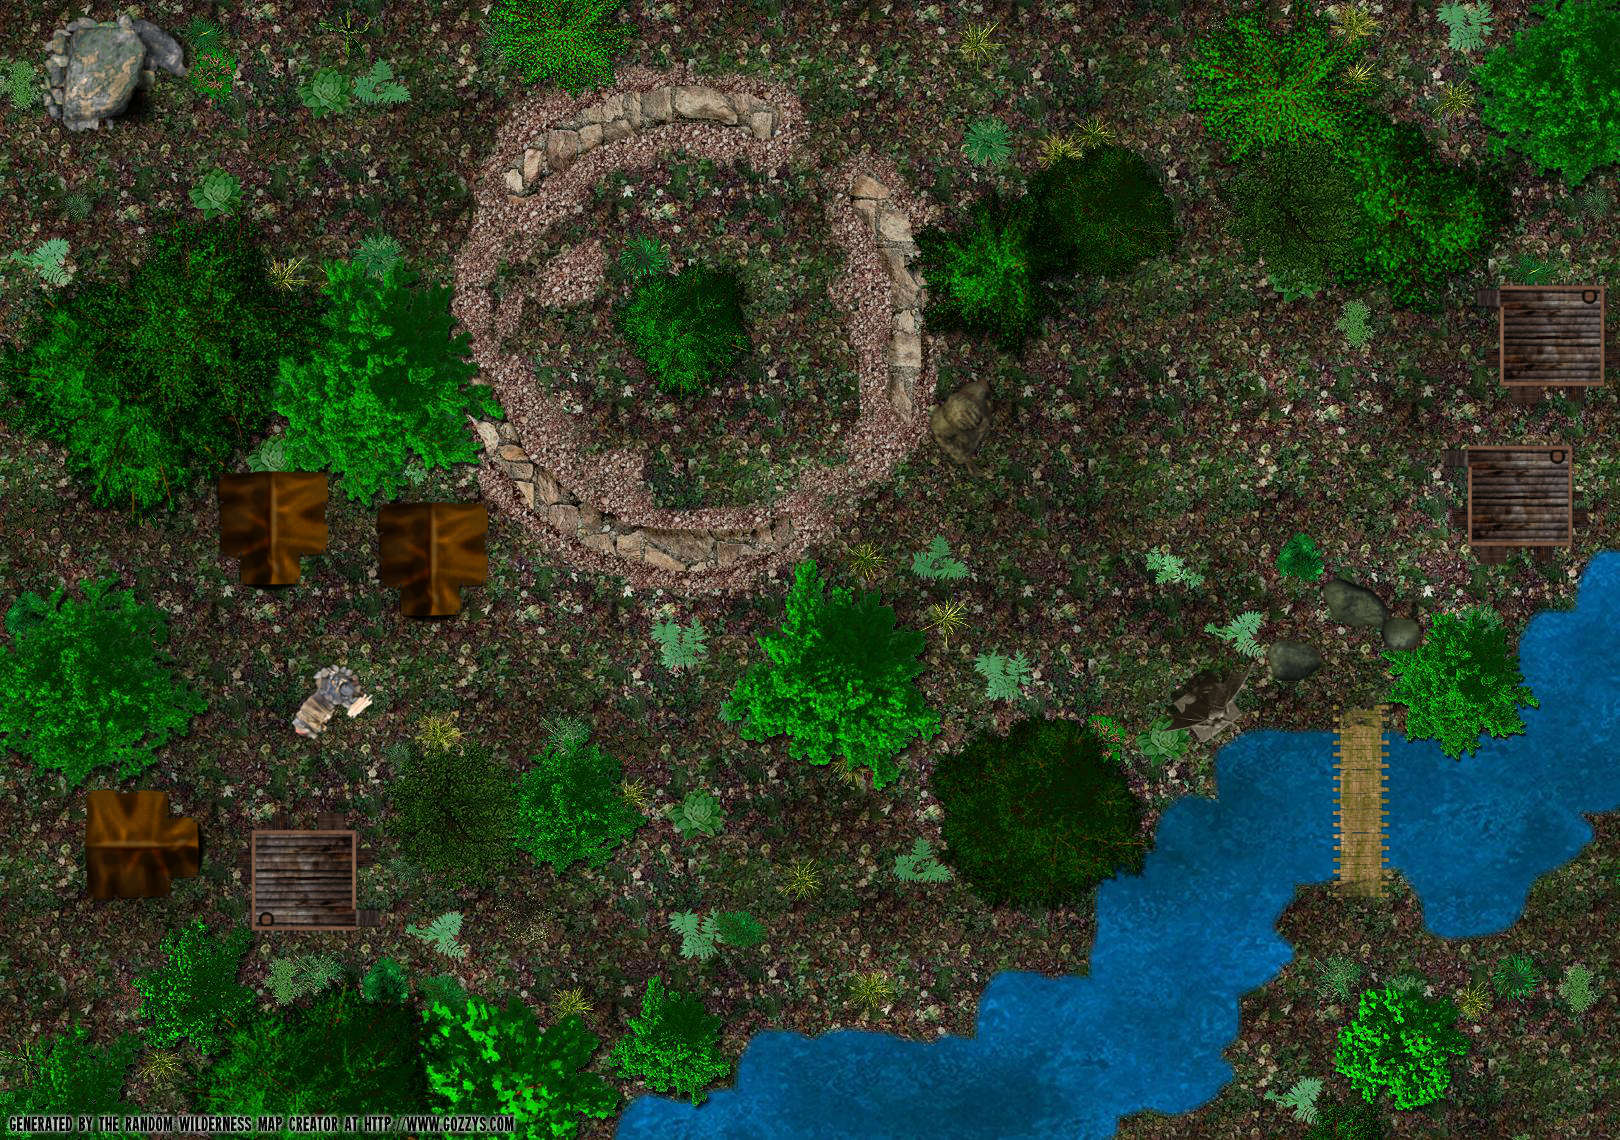
\includegraphics[width=1.0\linewidth]{./maps/Eisenkrafs-Bandits-Camp-(32+0+0).jpg}
\end{center}

\

%\vfill

The southwest hut and the tents hold ca 100enc worth of misc loot, with a total value of around 5g. Successful appraise gives a best value density around 2s/enc for 10enc.


\subsection*{The Cave}
%---------------------
The cave is unhealthy, some evil power lurks in the rock walls. For every 10r in the cave roll psy, with everyone failing getting a cumulative mod-1 to all rolls until they exit the cave. The mod is cumulative to a maximum mod-3, after that they start loosing 1 mana and 1 hp for every further failed psy roll. The mods are lost with 1 per round when outside the cave, but the mana and hp are restored with rest and time as usual.

This does not affect the bandits, but only a few of them can actually live in the cave without getting ill.

\begin{readoutloud}
There is a foul oppressing power in the air in here. Don't dwell too long.
\end{readoutloud}

The cave is divided in sections with locked bar partitions to make it easy to defend against intruders. The bars doors are str 15 to bash down, mod+3 to pick, or hp20 abs5 to destroy. Archers can fire through the bars at mod-1. Attacking through the bars with melee weapons is mod-6.

The secret passage doors are mod-6 to find by a passive perception roll but mod+3 if searching with a find roll. The passages are narrow and cost double mp and are mod-6 cramped terrain. The Secret door to the treasure chest chamber is locked str 8 to bash, mod+0 to pick, hp10 abs3 to destroy.

The bandits will retreat section by section and lock the bars behind them while they pepper the Heroes with arrows.

\begin{center}
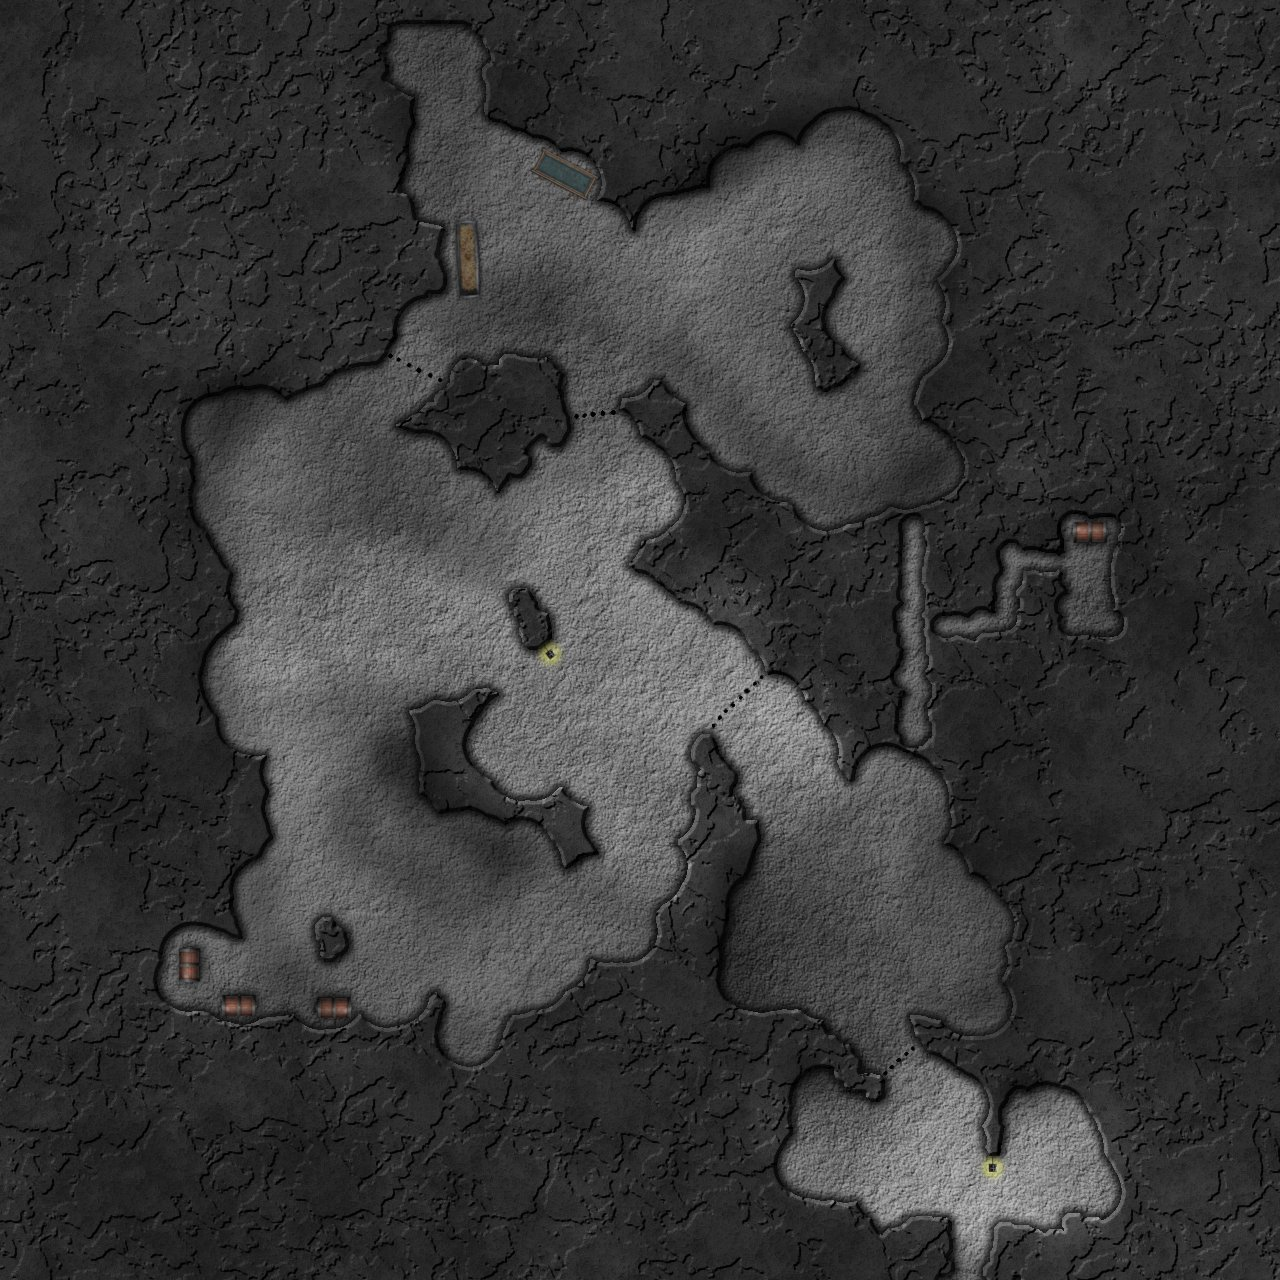
\includegraphics[width=1.0\linewidth]{./maps/Eisenkrafs-Bandits-Cave-(32+0+0).jpg}
\end{center}

\

%\vfill

The loot trough in the cave holds around 100enc of loot, worth ca 5g. A successful appraise gives a best value density around 3s/enc for 10enc.

The secret treasure chamber holds 3g 23s 160c, a ruby worth 15s, and a bracelet worth 8s. The bracelet is cursed. It seems to give the bearer cha+3, but it actually gives cha-3. If a Hero is using it and succeeds [+0,+3] he actually fails anyway. The player will hopefully notice that something is not right, sooner or later, as the GM says that obvious success rolls are failures...



\subsection*{Aftermath}
%----------------------
If the kidnapped siblings are returned to their farm the parents will pay 8s 15c as reward and be extremely grateful. This is all the money they have and make sure to impress upon the Heroes that the farm is poor and that the father literally upends and empties the small treasure box to pay them, handing over his last coin while crying, relieved to have his children back.
The father also tells the Heroes that he tried to get Baron Conq to send soldiers to free the children, but that the Baron refused.

If the Heroes travel to Baron Conq's castle to say that they have killed the Bandits they will be denied an audience, but the Master of the Guard will see them. If they have proof (severed heads, recognisable equipment, etc) the Master will pay 5s per dead bandit. He will only pay for bandits he thinks he recognises, and there is only 66\% chance per head. Roll as he carefully studies each head in turn.











%------------------------
%04b : The Summoning Site
%===============================================================================
%                               The Summoning Site
%                               ------------------


\clearpage
\phantomsection\addcontentsline{toc}{section}{04 summoning the demon}
\section*{04: The Summoning of Uchly Namen}
\chaptermark{summoning site}


\subsection*{Synopsis}
%---------------------
The Heroes get to the Summoning Site, with or without Dyslexia Marigt. They either get taken for sacrifice, or fight to free the girls. Then Uchly Namen arrives and the heroes must flee for their lives.

The Summoning Site is 14-19 leagues from Sleepy Cove depending on path.


\subsection*{If the heroes have come with Dyslexia Marigt as guards}
%-------------------------------------------------------------------
They have been travelling with Dyslexia Marigt and her RedGuard personal bodyguard. If they don't have horses or wagon by now she will provide a simple wagon to ride in.
\begin{readoutloud}
Approaching the old Gate Site you get an uncomfortable feeling as the landscape slowly shifts to become more odd. Vegetation changes, and the ground looks different somehow. As you approach a deep sunken valley Dyslexia Marigt says:\\

\textnormal{[sad old voice]:} This used to be a beautiful lake, before the Monster came through. The Summoning Magic somehow destroyed the landscape. I hope closing the rift will allow it to heal again some day.
\end{readoutloud}

A second RedGuard is waiting for them at the site. He greets them:
\begin{readoutloud}
\textnormal{[gruff stern voice]:} Welcome Madame. The ritual site is clear and safe.
\end{readoutloud}
This is surprising, why would she need another guard if she just hired the Heroes?

\

Dyslexia Marigt goes to the altar podium and begin preparing. After a while she asks the heroes to stand close "so that they will be safe during the ritual."
She then starts performing the initial steps of the ritual, which takes a few minutes. Then she gets sneaky: Pretending to continue with the ritual she casts slow on the Heroes. She wants to paralyse them, but she's not good enough to try that immediately. Once they are slowed she has more time to attempt Paralyse, as the RedGuards close in to make sure no Heroes attack or escape.
Roll for int to see if the heroes realise that she it not working on the ritual any more when she is starting to cast slow and paralyse. If any Heroes have the skill "magic", allow them to roll int+magic to see if he can figure it out.
Once slowed or paralysed the RedGuards will move in to grab the heroes and bring them to the altar. Capturing a Hero is a str resistance roll. Add Brawl and or Wrestle if available. If necessary the RedGuards will team up on the Heroes one by one.


\subsection*{If the heroes have come after Dyslexia Marigt, to free the girls}
%-----------------------------------------------------------------------------
Sam Slick has come with them to see what is going on. He will show them the site, but not fight initially. If they get into trouble he will offer to help them out for lots of money. If they pre-negotiate help he will settle for 10g, or 80\% of their total worth if they don't have 10g.

When they arrive Dyslexia is on the podium, chanting away. The girls are bound down lying on the altar. The two RedGuards stand by the podium, alert, scanning the surroundings.

The heroes now have a short while to try to get the girls free somehow. They can try to lure away the guards, or attack them from a distance, or attack Dyslexia directly somehow. Then they can try to grab the girls and run off with them.


\subsection*{The Fight}
%----------------------
Once the fighting starts Sneexious will first try to capture the Heroes as sacrifice material for the summoning/binding. She will try to cast Slow then Paralyse, to allow the RedGuards to capture the Heroes. If the Heroes manage to get aggressive enough to pose a threat the RedGuards will protect her.

Regardless of what the Heroes attempt it will probably not go so well, and Sam Slick will offer to help out:
\begin{readoutloud}
\textnormal{[Sam Slick shouts]:} Guys! You need any help? It's gonna cost you! Yes or No?
\end{readoutloud}
If they accept help he will charge them around 10 gold after they have escaped. More if he thinks they have enough. If they happened to take the broken Banor's Gate from The Wizard's Tower he will take that instead. It's \emph{not} recommended to try to stiff Sam Slick. It is likely to see you wake up without a head in the near future.

If Sam Slick gets involved he will throw a Blast Off! at Sneexious or the RedGuards, stunning them temporarily, allowing the Heroes to escape. He will urge them to run away and fight rear guard for a couple of rounds as they escape. If they decide to stay and fight anyway he will give up and run away himself. He will also run if he reaches 50\% hp.

Sooner or later Uchly Namen will come through, and then they will have to run away, with or without the girls. If they don't get it fast enough, let Uchly Namen swat one or two around for a few rounds, catapulting them around 5 squares away, knocked down, and dealing some crushing damage. E.g: swat attack 8 toavoid+2 dam 5 penetrating knockback 5. If after a couple of rounds they still don't get it just let him get angry and just stomp or hammer someone into the ground dealing d20 damage or so: hammer attack 12 toparry-9 toavoid-1 damage 20 penetrating consistent 2.

Sneexious will shout at them that they are imbeciles and fools. Without proper binding The Demon will be uncontrollable! He will lay waste to the entire region! Ruin to all! Death and Destruction!

\

The rest of the campaign follows the assumption that Deville Sneexious is not killed in this fight. But it's not a big deal if she is. Baron Conq has a backup wizard in case Sneexious would fail, try to betray him, wander away, or otherwise not be able to stick to the plan. Trymore John, a descendant of Trygain John, is also in Baron Conq's employ and ready to step in and take over Sneexious role should it become necessary.

If you want to throw your players a bone, let them kill Sneexious here. But she has the Armour Rune Amulet, Earthling and Invisibility spells, so it's not difficult for her to survive the Heroes and get away. Her two RedGuards will also defend her to the death if necessary, and Uchly Namen is somewhat under her control when he arrives, even if it will take time to forcibly argue and coerce him to immediately attack the Heroes.

Uchly Namen has just arrived. He's pissed at being summoned, he is disoriented from the transdimensional trip, and would preferably just eat whomever summoned him. Unfortunately he quickly realises that Sneexious and her RedGuards is under magical protection that he can't break, and she also has some binding influence over him, so the Heroes are the next best target for his frustration. Guilty by association.

\

But, very important \emph{do not} allow the Heroes to get their hands on the three stone necklace used for summoning and binding Uchly Namen. This would protect them from the Demon and somewhat wreck the story. If they manage to get it despite your best efforts, make sure some very skilled thief steal it in the depth of night sometime in the first couple of days. Baron Conq will never allow a band of lowly adventurers to foul his plans!



\subsection*{Aftermath}
%----------------------
Surviving the summoning by themselves gives the heroes 10xp each. If they are helped by Sam Slick they only get 5xp each. If they also rescue the girls they get another 5xp each.

Once the Heroes have fled and relaxed they can roll int to remember the tapestry in Honorbliz' tower. Yep, the same demon. Honorbliz must have info on how it was fought the last time. This if they didn't bother with the notebook.

Sam Slick will meet up with them later on. He tells them to keep an eye on Sneexious. And if they don't want to do it themselves he can do it for them, for a price of course, obviously.
Sam has now seen both the demon and the picture of the demon in Honorbliz tower. He thus knows that Honorbliz Wize was there fighting the demon. He can inform the heroes about it for 1 gold if they haven't figured it out themselves.

Due to the Heroes' interference, Uchly Namen is not properly bound. History repeats itself. This happened very similarly the last time he was summoned.
He won't be able to harm Dyslexia Marigt nor anyone close to her, but she cannot command him completely.
He will go on the rampage slowly. Working through farmsteads and villages.

Dyslexia Marigt will meet Baron Evilnius Conq in the old tower ruin and discuss the situation. Then she will send the wayward demon to destroy the Pawa castle, targeting primarily Baron Pawa and his Captain of the Guard.

Sam Slick can track her to the meeting place though, for a price, of course, say 5 gold? Or a couple of track rolls from the Heroes might do the same, say one roll per day?
Regardless of agreements with the Heroes, Sam Slick will sneak after Sneexious to see what is going on. He will warn the Heroes of the pending meeting, for a few gold.

\

In the mean time, Uchly Namen goes south, away from Sneexious who has some command over him. He comes across Kleinshof, where he wreaks havoc, eating a dozen or so inhabitants before enough people have managed to flee.
A few houses on fire. Some holes in roofs, some houses and barns razed. Random dismembered cattle and people spread out. Kleinshof is only 5 leagues due south of the summoning site.


\subsection*{Uchly Namen}
%------------------------
He is about four metres tall, very powerful, green scaly skin, glowing yellow eyes. Wings for gliding (not enough to really fly in this realm). Two arms with large clawed hands, two legs with large clawed feet.
When he is wounded he bleeds green-yellow glowing thick smoke for a few rounds. Wounds close 1hp per round. (Not regenerating, but the Heroes don't know that).
No use setting actual numbers to this monster. It will behave according to script.

\raggedbottom

\goodbreak \begin{samepage} \small \begin{verbatim}
===================================
Uchly Namen                 (named)
-----------------------------------
melee tohit+3 (very large, but mobile)
ranged tohit+6 (very large)
-----------------------------------
str  40      hp lots abs 4 skin
dex   8      m3 w6 r10 d15
con  30      stamina 30
int   7      vision 30 arc 180deg, infra soul
psy  18      mana 30
per   8      ap 6
cha   3      xp --
----------
swat        10 dam  7 pen 2, fast+1, knockback 3+1d4sq, min 2dam penetrating
slash        8 dam 14, knockback 1d3sq, min 1dam penetrating
grab         8 dam  6, crush each round dam 8 pen 2,
               break free is str vs 10,
               or get thrown away 5+d5sq taking dam 2+1d3 penetrating.
bite         - dam 10+d10, penetrating 2, automatic hit if grabbed/held
parry grab   8 will rip weapons out of hands, auto success
parry swat  10 fast+1, rip weapons out of hand on 10 vs str resistance roll.
scary        - psy-3 roll to attack, only psy-0 after succeeding once at mod-3
roar         - psy or flee 1d3 rounds, psy-3 not to back off 1 round.
ancient     11 well spoken, if you know the language
consistent   2
===================================
In maptool: set hp 1000 and con 0
Then adjust and update to 400 for "damaged",
                          200 for "seriously damaged",
                           10 for the last strike that Bling SwordSlash makes
                              to "kill him off". Remember that Bling has Über!
\end{verbatim} \normalsize \end{samepage}

\

And, in case Deville Sneexious dies off, here is Trymore John. He's a wimpish man and doesn't seem to be much of a threat, but he has impressive defences and is \emph{very} alert for any potential threat.

\goodbreak \begin{samepage} \small \begin{verbatim}
===================================
Trymore John                (named)
-----------------------------------
str   4      hp 12 abs 2 (exotic rune ward)
dex   5      m1 w3 r5 d7
con   4      stamina 6
int   9      vision 28 arc 240 (set human good)
psy   8      mana 22
per  12      ap 6
cha   4      xp --
----------
quick        3
mobile       3
rapid       12
literate     9
Common      12
Ancient      9
Svartlingo   7
counting     8
histography  7
ride         6
travel       4
avoid       11 yield+4
knife        7
Teleport     wannagohome, recall
----------
magic        6

blinding cloud 8 cast 1r 4m, range 2+1/m, dam 1 penetrating, duration 5r
                 All attacks into the cloud are at mod-6 per
                 distance to target (max-range*6).
                 Damages everyone in the cloud, including caster.

-----------------------------------
Amulet of Gone: gives Blink (adaptive, fast, instant)
                3ap activation, draws 5mana, max blink duration psy rounds.

Spoon of Blandness:  gives Bland 8 (int-8 to attack bearer first)
                     if the wielder holds no other weapons
                     dam 2 abs 8 parry+2
                     use with any melee weapon/brawl skill

===================================
\end{verbatim} \normalsize \end{samepage}




\flushbottom


%\begin{center}
%\vspace{1 cm}
%\includegraphics[width=1.0\linewidth]{./maps/Summoning-Site.jpg}
%\end{center}
%
%\














%-------------------------------------
%05 : The meeting, Old East Tower Ruin
%===============================================================================
%                              Old East Tower Ruin
%                              -------------------


\clearpage
\phantomsection\addcontentsline{toc}{section}{05 the villains' meeting}
\section*{05: The Meeting -- Old East Tower Ruin}
\chaptermark{villains' meeting}


\section*{Synopsis}
%------------------
The Heroes will sneak up on a meeting between Sneexious and Baron Conq. They will hear them discuss the assault on Pawa. The will hear Sneexious perform the command to send the Demon to attack Pawa Castle.


The Old East Tower Ruin is 8 leagues due north of The Summoning Site.


\section*{The Meeting}
%---------------------
Sneexious is waiting near the ruin for a couple of days before Baron Conq arrives.

The Heroes arrive just in time to follow Sneexious to the ruin and meet Evilnius Conq's guard. Then the Baron Conq himself emerge from the ruin when it is safe:

\begin{readoutloud}
\emph{Conq [expectant]:} So, Witch. Has it been done. Is the Demon here, ready for my command? \\
\emph{Sneex [carefully]:} Yes Baron. I have summoned the Beast. Uchly Namen is once again walking this land. \\
\emph{Conq [evil, pleased]:} Excellent. Well done witch. Here is your 100 gold, as promised, for the first part and you expenses. \\
Now, command it to attack Castle Pawa. I want that annoying old man dead. Eaten, if possible. Command the Beast not to rest until the Baron Pawa and his Captain of the Guard both are dead. But make sure it does not destroy too much of the castle. I don't want to spend half of Pawa's treasury having to rebuild it once I ..."rescue"... the city from its predicament. \\
\emph{Sneex [careful, determined]:} Yes, lord. And, as soon as your spies confirm the ruination of Castle Pawa, I expect to have the rest of the payment forthwith. I will have to hurry back to Banish the Demon, and I want my money before my leverage leaves the scene. \\
\emph{Conq [disdain]:} My dear Sneexious, I'm hurt that you do not trust me. Have I not always settled my debts? \\
\emph{Sneex [irritable]:} Your way of settling your debts is not always to the liking of your creditors. And seeing as I'm one of them now, I'm not inclined to be lenient on the details of the payment. \\
\emph{Conq [bland]:} Of course, you ride back with me immediately, once you have commanded the Demon of course. \\
\emph{Sneex []:} Settled then. \\
\end{readoutloud}

Sneexious now begins a short incantation. She opens a command gate to the demon's position, then shouts her command, in an ancient language, to the demon, who will then slowly have to comply, for a while.

In the next couple of days Uchly Namen will make its way to Castle Pawa and begin the assault.

\

Once the command ritual is completed, Conq's entourage, and Sneexious, will ride off north.

It is unlikely that the Heroes will be able to fight through the RedGuards, even with the (if paid well) aid of Sam Slick. They might be able to interrupt the proceedings, but both Sneexious and Conq's guards will be very intent on killing them if they are found.

Uchly Namen is now commanded north east from the region south of Kleinshof. But he's very quick, and the Heroes won't be able to get to Castle Pawa in time to warn them. If they go quickly they can reach it just as the battle is still raging inside.


%\begin{center}
%\vspace{1 cm}
%\includegraphics[width=1.0\linewidth]{./maps/Old-East-Tower.jpg}
%\end{center}
%
%\


















%------------------------------
%06 : The Battle of Castle Pawa
%===============================================================================
%                       Castle Pawa : Attack of Uchly Namen
%                       -----------------------------------


\clearpage
\phantomsection\addcontentsline{toc}{section}{06 attack on Castle Pawa}
\section*{06: Castle Pawa -- Attack of Uchly Namen}
\chaptermark{castle Pawa}


\subsection*{Synopsis}
%---------------------
The Heroes might not be here when it happens. Uchly Namen will attack the castle city. After many hours he will manage to kill Baron Pawa and the Guard Captain. He will then eat some more people, sit and sleep on the gate remnants, then leave around lunch the next day.

If they hurry from the Old Eastern Tower meeting to Castle Pawa they can get there in time to see the carnage, and to try to fight the Demon a bit if they want.


\subsection*{The Attack of Uchly Namen}
%--------------------------------------
Uchly Namen will attack in the Dead of Night. He will start by razing a farm nearby, then pound down the gate and some surrounding structures. Well inside he will start eating people and some cattle left and right until he must search out his commanded targets. It will take him hours to actually figure out who he is supposed to kill. He can't speak the language, and it takes a while before he finds a scholar and manages to torture him into translating for him from his ancient language. This scene is rather weird. He will be picking up people left and right, shouting at them \emph{[in ancient:] DO YOU UNDERSTAND WHAT I'M SAYING?}, shaking them, trying again, then tossing them aside when he they just shout and scream.

Many witnesses will be able to repeat the horrible battle cries of the Demon. \emph{[ancient:] Why don't you stupid fleshlings understand me?}. They will describe the process in detail.


\subsection*{If the Heroes are there}
%------------------------------------
The Heroes will not have a chance to reach Castle Pawa before Uchly Namen, but they can get while the battle still rages. The Heroes have a chance of limiting the destruction of Castle Pawa and it's inhabitants. If they have figured out that the spear and shield from the last banishment of Uchly Namen is kept in the great hall in Castle Pawa they can perhaps find it during the mayhem and use it to battle the Demon. They are not skilled enough to really do any significant damage to it, but the Demon cannot easily damage the shield carrier. The demon will just whack the shield bearer away all over the courtyard until he gets tired or banged up enough to stop coming after him. If the Spear Wielder manages to score several hits on the Demon it will leave early, limiting the damage to the castle. But not before he has killed Baron Massa Pawa and the Captain of the Guard.


\subsection*{Aftermath}
%----------------------
Once Castle Pawa is attacked the spies of Baron Conq will ride home (20 leagues) during the night and early next day. By the afternoon Conq will have paid Sneexious, and she will set off. Officially she is on her way down to the summoning site to banish the demon. However she knows she will not be able to do so. She also knows that Baron Evilnius Conq will not let her get too far with all that gold, and that he has surely sent guards/assassins after her, perhaps to kill her and take the money once the demon is gone, and surely kill her if she does not banish the demon. Her only way out is to actually get down to the summoning site and then somehow trick or kill Conq's agents. Likely she will try to summon the demon down there and then try to have him kill the potential assailants.

But first she goes to Sleepy Cove "to pick up supplies for the Banishing Ritual". She will sell off most of the last of her stuff, and pack and send away the rest. She will stay in Sleepy Cove long enough for the Demon to think she is there and come looking for her, but she will be gone by the time he arrives.

Baron Evilnius Conq will ride out the next day, leading his army towards Castle Pawa, to "rescue" them from the horrible attack of the demon. It will take him about two days to ride the 20 leagues north of the forest. He will leave a small guard at home in Castle Conq. Arriving at Castle Pawa he will make a pretty speech, then promptly install himself as the new ruler. Some voices will be raised about sending for Heirling Pawa, the son of Massa Pawa. Those raising the concerns will be invited to a council, from which they will never leave. Conq will then tell the city folk \emph{"Those heroic citizens have taken it upon themselves to find and bring back the rightful heir of the land. In the mean time I'll do my best to protect you from the foul horrors of beyond."}

Uchly Namen is mighty irritated at Sneexious for commanding him to mess with Castle Pawa. Not only did he get hurt quite a bit from all the soldiers and siege weapons. He also had to spend hours figuring out whom to kill.
He will now head west, drawn to the place where the summoning/binding necklace was again put together again and charged. Drawn to Sleepy Cove and the cabin where Dyslexia Marigt lived, and worked on the necklace. He wants to figure out a way to kill Sneexious, and he has some ideas. He is wounded, weak, and pissed off.

Following the road he will first pass through Merna, staying a bit to wreak havoc. Then continue to Sleepy Cove.


%\begin{center}
%\vspace{1 cm}
%\includegraphics[width=1.0\linewidth]{./maps/Castle-Pawa.jpg}
%\end{center}
%
%\

















%--------------------------------------
%06x Intermission - demons on the loose
%===============================================================================
%                            Demons on the loose
%                            -------------------


\clearpage
\phantomsection\addcontentsline{toc}{section}{intermission, demons on the loose}
\section*{Demons on the Loose}
\chaptermark{demons}


\subsection*{Synopsis}
%---------------------
Grey Stalkers might have gotten through the portal Sneexious opened. They will lay in ambush for the heroes when they travel from Castle Pawa.


\subsection*{The Ambush}
%-----------------------
If the heroes interfered with Dyslexia Marigt before she managed to properly complete the summoning ritual, which is very likely, the gate is left a bit ajar and a pack of Grey Stalkers have managed to get through. They will ambush the heroes when they leave Castle Pawa to track down the Demon.

The Grey Stalkers are dangerous in that they blink out defensively and it is a bit annoying for the players to keep track of where they are. This also makes it more difficult to hurt them in melee fights. They also try to separate the Heroes by doing their tackling horn charges and throwing the targets away from each other.

Open with the small ones on the road, charging, and the big one placing an explosion in the middle of the heroes. That is a nice good start to the fight. Remember that the Stalkers are intelligent, have hive vision, and will coordinate their fight very well.

It is possible to talk to the demons if a character can speak ancient, but the Heroes must present something very nice for the stalkers to be interested in dealing with them. Food, magical thingies, etc, but not gold.


\subsection*{The Opposition}
%---------------------------
At this point the Heroes should be quite powerful, but the Grey Stalkers are difficult to fight. The horn charge, blink, teleport, and explosion effects make them quite deadly. One can charge then blink out while the next charges, staggered attacks, then they blink in together. And as they get damaged they flee back to the big one by teleport.

It's likely that the Heroes will only be able to drive the stalkers away.

\begin{samepage} \vsmall \begin{verbatim}
Grey Stalkers:
  big grey stalker         1x   as listed in the rules
  grey stalker             5x   as listed in the rules
\end{verbatim} \normalsize \end{samepage}


%\begin{center}
%\vspace{1 cm}
%\includegraphics[width=1.0\linewidth]{./maps/Demons-Road.jpg}
%\end{center}
%
%\
















%-----------------------
%07 : Defend Sleepy Cove
%===============================================================================
%                              Battle of Sleepy Cove
%                              ---------------------


\clearpage
\phantomsection\addcontentsline{toc}{section}{07 battle of Sleepy Cove}
\section*{07: Battle of Sleepy Cove}
\chaptermark{battle}


\subsection*{Synopsis}
%---------------------
The Heroes might figure out a way to save Sleepy Cove by using the spear and shield from Castle Pawa. Otherwise they will have to watch as Bling SwordSlash extorts huge amounts of money and then goes into another Heroic Battle and forces the demon away, somewhere else, not his problem.


\subsection*{Uchly Namen arrives}
%--------------------------------
Scared villagers will be running by, screaming. The town will be mostly empty by the time Uchly Namen arrives on the main street. He is visibly hurt, but still fights like a champ. He ruins houses, eats cattle, and swats people left and right.

The Heroes will form up on the Main Street to stop him. Some brave spectators will stand around, and Bling SwordSlash will be resting with a glass of wine off to the side.


\subsection*{The Battle}
%-----------------------
If the heroes attack him with the spear and shield they might hurt him a little every now and then, but take damage themselves as they fly left and right from his powerful attacks.

When the heroes have had enough, the demon is almost dead. He has problems standing, he falls every now and then, and slowly rises to fight on. Strange smoke wisp from his many wounds.

This is when Bling SwordSlash seizes the moment. He takes the spear and shield from the heroes:

\begin{readoutloud}
You should leave this work to Great Men, of Substance, such as Myself! I shall Save the day, and Protect All the people of this quaint little Village! \\
Now, Foul Beast, prepare to meet your Doom! I shall thwart thy evil marauding!
\end{readoutloud}

He then proceeds to advance on the demon. He dodges two attacks then plunges the spear deep into the chest of the beast. The Demon dies, falls on its back, and the scene ends with Bling SwordSlash posing beside the beast with one foot on the shoulder, as the villagers gather to celebrate him.


\subsection*{Aftermath}
%----------------------
In the end Bling SwordSlash gets 50 gold for slaying the Demon. Sleepy Cove and the other villages pool their money. The Heroes gets nothing of course, since they were saved by Bling SwordSlash.

The villagers have already plundered what's left of Dyslexia's house, as well as the delayed shipment from the Trade Town. If the Heroes bring up the money, they are reminded that they were working for the witch, and might be accomplices. Especially if they push the issue... In the mean time they are treated well, but still has to pay for the rooms at Sleeping with the Fishes, until they have recovered enough to travel in search of new adventures.

\

In the future, the heroes will often hear the ballad of Sleepy Cove, where the valiant Bling SwordSlash defeats the beast Uchly Namen in single combat, and where many lesser men have failed, he succeeds with heroic skill.












%-----------------------
%XX : Appendix: Playthrough
%===============================================================================
%                                 Playthrough
%                                 -----------


\clearpage
\phantomsection\addcontentsline{toc}{section}{Appendix: playthrough}
\section*{Appendix: Playthrough}
\chaptermark{playthrough}
\label{sec:playthrough}

\raggedbottom

The playthrough was originally posted as a "Running Campaign" reporting on the maptool forums (091210-100518). Unfortunately, the file hosting was removed so all the illustrations and screen shots disappeared, but the original text is still available. Here I've done a little clean up and put it together. I've also found a source for the lost illustrations and screenshots.

Note that I did some fails as a GM when leading this campaign, and that I changed a few things in the campaign from post game notes. Hence, some details in the chronicle differ from what is likely to happen resulting from a new playthrough.


\subsubsection*{Sessions 1-2: Welcome to Sleepy Cove, Here be Goblins}
% originally posted 091210
\noindent\small
The first sessions are always a bit of a hassle with technical issues, etc, that take up a majority of the time. The folks using linux have had no problems yet. Those using vista are encountering significant weirdness, although most are not related to the game tools. One guy running w7 gets disconnected every now and then from maptool, but has had no other technical issues.
It always takes a bit of time to get things set up and running, and getting people used to the tools. That's all to be expected I guess. I expect the future sessions to run smoother. Running with: maptool-1.2-b32 (waiting for that stable 1.3 ?), jarnal-917, skype.
\normalsize

The stalwart heroes Mandak, Datarian Blood, and Nostromo have set out upon their first adventure as Fresh Hero Wannabes. Their first stop was the small village of Sleepy Cove, where they after some time located the old scholar and wise woman Dyslexia Marigt. The sweet old lady explained the horrendous back story and the tasks the Heroes would be required to undertake as her employees. As she talked the glitter of future gold got a bit much for Nostromo, who embarked upon a resilient haggling campaign.

\begin{center}
\vspace{0.5 cm}
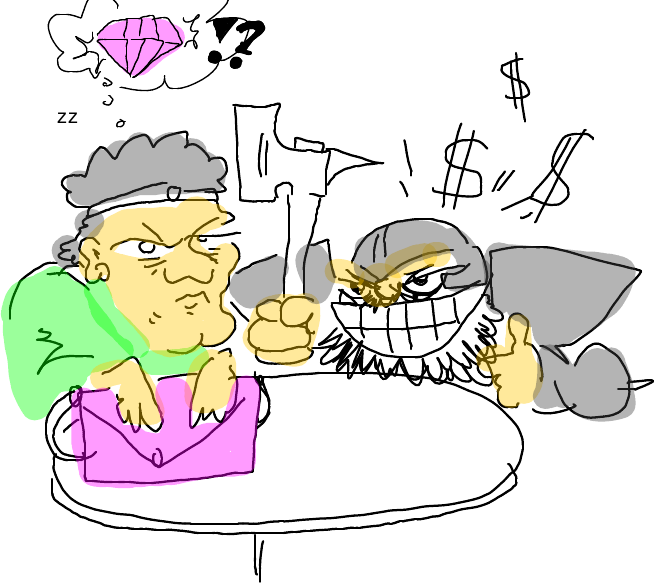
\includegraphics[width=0.7\linewidth]{./figs/playthrough/negotiate.png}
\vspace{0.5 cm}
\end{center}

After the eager newbie Heroes had secured employment, they merrily started making the village a slightly less sleepy and safe place to live. In the end they stumbled upon the General Store, where they proceeded to purchase the bare essentials of dungeon hacking: bags and provisions, under excessive haggling and some name calling. Once sufficiently supplied they set out towards the South Forest, to find the Goblin Bandits.

\begin{center}
\vspace{0.5 cm}
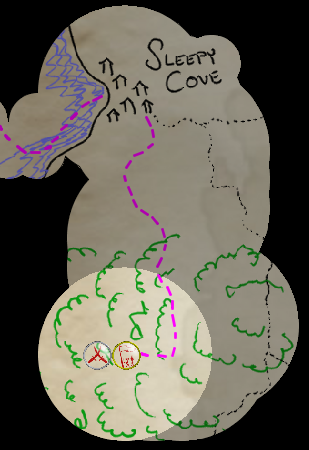
\includegraphics[width=0.4\linewidth]{./figs/playthrough/travel-goblins.png}
\vspace{0.5 cm}
\end{center}

On the the second day of travelling, they noticed goblin tracks, and the next day they moved in on the camp site. After carefully advancing close enough to the bandits' camp to hear the goblin gibberish and smell the camp fire, the honourable Heroes stopped and whispered amongst themselves. After a protracted debate they finally devised an infallible plan.

\begin{center}
\vspace{0.5 cm}
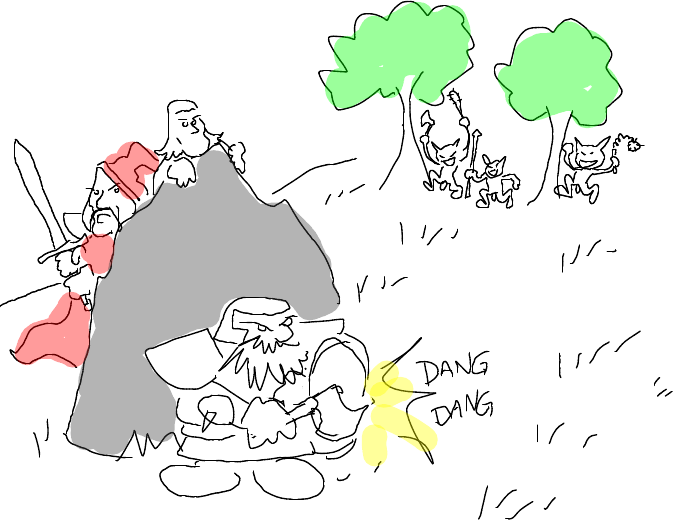
\includegraphics[width=0.7\linewidth]{./figs/playthrough/sneaky-plan.png}
\vspace{0.5 cm}
\end{center}

A bloody battle ensues, where the Weapon Wielding Heroes slowly maim, kill, and slaughter Goblin Bandits left and right. The rest of the goblins finally realise their perilous predicament and flee towards north east, towards their cave.

What will happen next? Stay tuned for more gore, guts, gold, and glory!


\subsubsection*{Session 3: Nostromo's Slaughter of Goblins}
% originally posted 091216
The third session was short and depopulated as only Nostromo showed up. Datarian Blood had attempted a pre-emptive strike against the mad pig disease and lost, Mandak was awol, Piggelina was writing on her next research article, and an unnamed wizard was returning home from a consulting job in the far reaches of Nowhere.

Nostromo was not deterred by the lack of compatriot support, and in a gust of hubris the ArmourDwarf slooowly chased the goblins into their cave. After which he commenced to light a fire just inside the opening, hoping to smoke them out. Unfortunately the cave entrance designers and ventilation technicians had already thought of this eventuality and the clever plan turned out to be futile. \emph{This would so totally have worked if he had studied enough Dungeoneering} :)

Nostromo then grabbed his trusted heavy axe and shield and advanced into the horribly stinking dark cave. Going into a side tunnel he spotted the Bandit Boss standing a bit away, taunting by waving his derriere. As he moved in, intent on bloody murder, Nostromo soon also noticed the other 5+ goblins as they emerged from their hideouts to ambush him.

Taking some damage from the initial assault of the numerous Goblin Bandits Nostromo slowly backs away into a tunnel which proves to be a much more suitable battle ground. During the tunnel fight he quickly cleaves one goblin and decapitates another, leading to the much slower and more careful advance of the rest. Just as our stalwart Hero is sure of his position he hears the rapidly closing roars of a wolf, and moments later the ragged beast comes leaping through the goblins for a violent attack.

How will this end? Stay tuned for more smoke, stench, and sneaky savages...


\subsubsection*{Session 4: The RedStone and Stinky Bird Monsters}
% originally posted 091219
Nostromo, the ArmourDwarf, readies his heavy axe as he backs away, down the cave tunnel. The goblins take a side step to let the wolf through to attack the invader. Rapidly the canine beast leaps onto Nostromo and furiously tries to bite him. Nostromo just forces the wolf back with his enormous shield, and then makes a clean decapitation.

In the mean time the Bandit Boss and what is left of his group have formed battle positions and they attack as the wolf dies. Nostromo takes cover behind his shield as the arrows rain down around him, then defends against a few attacks from the goblin chief, before giving him a lethal cut.

As the goblin boss MuchKlajn GoBoss dies he screams:
\begin{readoutloud}
Aaargh, me Die, Like Stinky Pie.\\
You die Too, You Stinky Shoe.\\
You be StinkiEst of All !
\end{readoutloud}
After which Nostromo stomps out his life, crushing his head under one large armoured boot.

The remaining goblins retreat into the cave to regroup, and Nostromo slowly follows. A pitiful battle ensues before the archers realise that they really cannot penetrate his armour with their weak bows. Then they flee, loosing one to the axe of the Relentless Dwarf.

As the goblins flee out of the cave Datarian Blood just logs on. The paladin blinks a couple of times where he stands in the sunlit clearing of the goblin camp, and then realises he now has four goblins running towards him from the cave opening. He starts moving towards them. Noticing the red clad paladin, the goblins veer left and escape into the forest in a few rounds.

Nostromo and Datarian Blood start searching the stinking cave. The find a pile of loot and rubbish, three dead bodies, an offal pit, and some minor goblin belongings. Looting some coin and packing their sacks full with smelly stuff, they also investigate the swollen ripe corpses of the lost adventurers. Hidden in a secret pocket they find the RedStone and realise they have just completed their first real Heroic Mission. They also notice that Nostromo smells really \emph{really} bad.

Later that day they are walking north through the forest, on their way back towards Sleepy Cove, when suddenly they hear a strange cooing sound. Failing their int rolls they have no clue what it is, and neither of them paid any attention in school during their monsterology classes. Datarian takes some time to cast healing on Nostromo to get him back into perfect health.

As they prepare for battle a large IffyGriff appears through the heavy under-brush. They form up ready to fight the slowly advancing monster when Nostromo notices the fast running shapes of two smaller IffyGriffs circling around them. The next round Datarian sees a third circling IffyGriff chick. They are getting a bit uncertain about the wisdom of engaging when the IffyGriffs charge them simultaneously from all sides.

A bloody and ferocious battle ensues. The heroes try to keep their stomach content down in spite of the oppressing stench of the horrible IffyGriffs. Between regurgitations they attempt to chop the horrid little bird monsters into fine pieces. Nostromo's enormous shield and thick armour really saves his life as he for some reason turns out the be the target of all the critters. After a few rounds they have managed to slay the large mother IffyGriff, and the chicks make ready to flee. One dies as he is not fast enough to disengage, while the two others get away into the surrounding forest.

Searching the area they find a stinking nest and picks up three large smelly eggs, packing them amongst the other loot before continuing on their way back to Sleepy Cove.

Well back they take a room and some food at the "Sleep with the Fishes" inn, where Singalot the Bard is performing ballads and songs on the Heroics of Bling SwordSlash. Bling himself is a bit tipsy, surrounded by dreamy eyed local girls. The locals are not impressed by the horrendous stench of the two adventurers. Despite repeated baths and aggressive scrubbing Nostromo just cannot get the odour out of his skin, and his night's sleep is interrupted by rats coming to gnaw on him.

The next day they sell their loot under a barrage of haggling, then proceed to deliver the RedStone to Dyslexia Marigt. The old scholar is very happy they found the stone, sorry about her previous hirelings, and pays them the seven gold for the stone. Serving them milk and cookies she explains again that the GreenStone was supposed to have been delivered already by Coal-Black-George, but that he must be occupied. Can the heroes please go to Eisenkrafs to pick up the stone? She also gives them one gold to pay for it.

The stalwart heroes now take a day of rest and recuperation to spend their brand new silver and xp.


\subsubsection*{Session 5: Let's take a Trip to Eisenkrafs}
% originally posted 100108
The Heroes burn through their coin pouches shopping for gear before they set out north towards the mining village of Eisenkrafs to find Coal-Black-George. Since only Datarian Blood and Anomali are in attendance the gang is lacking a tracker. They stumble myopically along the north road until they, a couple of days later, get ambushed just after a pleasant lunch.

\begin{center}
\vspace{0.5 cm}
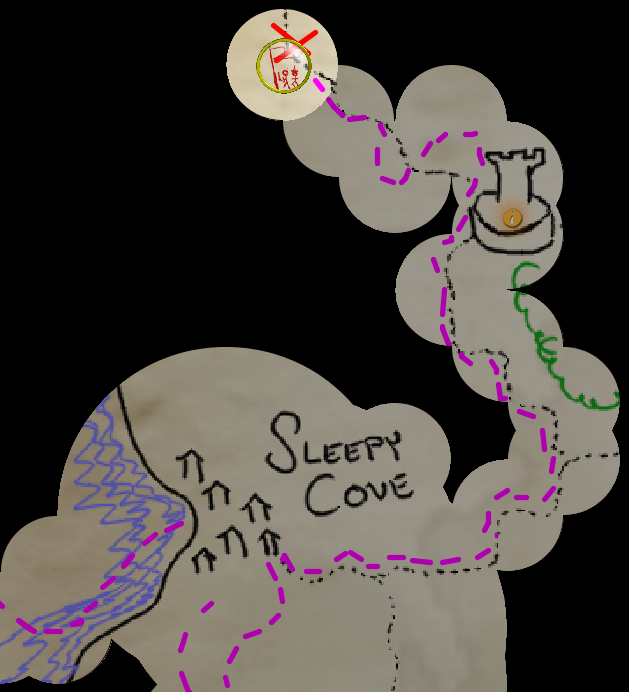
\includegraphics[width=0.5\linewidth]{./figs/playthrough/travel-eisenkrafs.png}
\vspace{0.5 cm}
\end{center}

Four BiteRunners come charging at them from the eastern grass plains. The two heroes take cover by a rock, and quickly dump their travel packs to move easier. Datarian stands ready with his sword and shield, and Anomali has hung his bow in favour of his staff. A furious battle ensues, where the very fast and mobile BiteRunners circle around them and make quick sporadic synchronised attacks. Ten rounds or so later Datarian is injured while they have managed to kill one of the monsters and wounded two others. The monsters start fleeing, but one of them leaps on top of the rock where the heroes have stashed their provisions, and make off with a sack of rations. And with that all the critters quickly disappear back into the east grass plains.


\subsubsection*{Session 6: Into the Mines... Wait, No one though to bring a Torch?}
% originally posted 100129
The heroic three: Nostromo, Anomali, and Mandak head north after the assault and escape of the biterunners. The monsters unfortunately managed to escape with a pack of provisions, so the heroes must now share what is left. They are on their way north to Eisenkrafs to talk to Coal Black George who was supposed to show up in Sleepy Cove to sell the GreenStone earlier, but never arrived.

After a couple of days they reach the sorry mining village of Eisenkrafs. The air is heavy with smog, lost hope, and destitution. They wander aimlessly through the desolate village for a while before going over to the mining yard. There they talk with the offensive mining foreman Gebbhard Goebbels, who says Coal Black George has not shown up for his shifts the last week or so, but that he doesn't know where he is.

The Heroes then go to the beer house and start handing out copious amounts of beer from the barrel Nostromo has been bringing along. The taste of decent foreign beer slowly manages to loosen the tongues of the grimy old miners gathered in the establishment. They say Coal Black George is a good miner, but that he has been missing for a while. Gebbhard Goebbels, the boss, should know where he is. The rumour is that Coal Black George has been working in the closed down sections of the mine all by himself, and that he got eaten by The Worm.

Back at the mine yard the Heroes again talk to Goebbels. He says his men has searched the village and Coal Black George's hovel, but found no trace of him. Perhaps he has left the village? The Heroes refuse to believe that, and argue to be allowed down the mine. Goebbels says George sometimes went by himself to shaft 5-1 for some reason, perhaps he has met with an accident. Goebbels tries to warn them about all the horrible dangers that lurk deep in the mine, but they won't listen. At last Goebbels gives them a healing draught for George if they find him hurt, and sends one of his men to help them down into the mine and the closed down areas.

After reaching shaft 5-1 the miner rigs a long rope ladder and the Heroes descend into the darkness below. They emerge into a natural cave that seems to have once been in use, but abandoned long ago. The rope ladder suddenly drops from above, and coils into a heap on the floor. The way back up just became much more difficult.

Having forgotten to buy light sources they have to make do with the meagre ghostly light from softly glowing fungi growing on the walls and floor in small patches. This is quite enough for the elves, but Nostromo has a bit of difficulty. They set out into the darkness of the cave.

Nostromo has to go walk his dogs, and takes his leave for the evening, while Mandak and Anomali push on. They soon encounter a large cave worm. A slow slobbering foul beast. While fighting it they get ambushed from behind by large spiders. Another worm soon joins the battle. After 20+ rounds they have slain the arachnids and the worms, avoiding both the spider venom and the acidic worm spittle.

They venture further into the darkness...


\subsubsection*{Session 7: Who Needs Light? We Fight Trolls in the Dark!}
% originally posted 100225
Nostromo the ArmourDwarf and Datarian Blood the Heroic continue deeper into the natural caverns below mine shaft 5-1, searching for Coal Black George and the GreenStone.

They soon enter a large natural cave room, where they attract the attention of many shiny large bugs. Large for bugs at least, but not really that large. While trying to cleave the annoying bugs they wake an old cave troll that slept further off, behind a large boulder.

During some 20 hectic rounds they valiantly defend against and wear down the monstrous troll, while being harassed by the many bugs that insistently find gaps in the armour. They finally manage to corner the troll by a intercepting and blocking his escape route, and Datarian places a heroic final blow that kills the troll dead. Then they stay to mop up the bugs. Datarian have taken significant damage during the battle and is in poor shape.

Afterwards they rest and recover while Datarian slowly casts a few healing spells to get them back to combat readiness. This takes them around 20 rounds of healing and some 10 rounds to rest, after which they continue to explore the caverns.

Their final act for the evening is running into three large spiders. Now the evening has drawn towards night and it is time to go to bed.


\subsubsection*{Session 8: Spiders, Bugs, and Another Troll.}
% originally posted 100302
Datarian Blood and Anomali have gathered for an unusually long session. Three hours and over 100 rounds of bloody mayhem as they push on deeper into the natural cave system below shaft 5-1.

The Heroic adventurers resume their exploration at the point where they had just encountered a group of spiders closing in. They quickly and safely hack the spiders to bits and pieces, managing not to get poisoned and only a bit entangled in the spiders' sticky webs.

After the murder of spiders they continue south and soon encounter a half dozen bugs. Nasty critters, and so they set about killing them off, only to realise that these bugs also come with an old cave troll. The bugs nibble at the health of the Heroic Duo, and then suddenly the troll manages to land a heavy blow on Datarian Blood, pushing him to the brink of death. The heroes now flee for all they are worth, pursued by the blood thirsty troll and bugs.

The salvation comes in form of an old and rickety wooden bridge. The troll is unwilling to cross and Anomali engages in a protracted hit and run tactic to wear it down with his bow. Datarian strips down and starts casting his healing magic to recuperate, taking a long time to do so in his poor state of health.

\begin{center}
\vspace{0.5 cm}
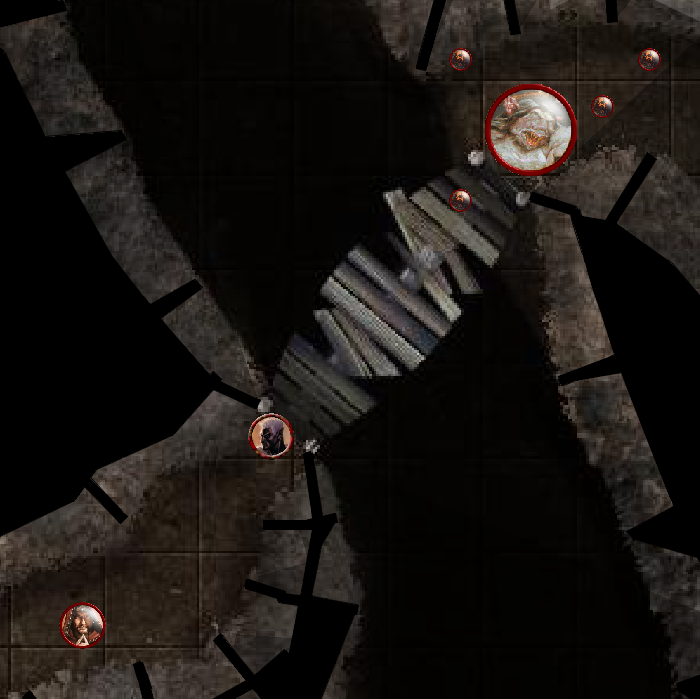
\includegraphics[width=0.7\linewidth]{./figs/playthrough/bridge-troll.png}
\vspace{0.5 cm}
\end{center}

After a good while the severely wounded troll has tired of the fruitless battle against Anomali and fled. Anomali has taken a while to combat the bugs and finally manages to kill them off with the help of Datarian. After a bit of resting they pursue the troll back to its lair and brutally slay it.

Soon they find a potential way out of the cave system, but realise that they will need proper digging equipment to get it cleared in any reasonable amount of time. Preparation is lacking. So instead they loot the troll lair before returning to where their cave adventure started. They are not good enough at climbing to attempt the now rope-less shaft, so instead they go exploring for another way out further off. Just as the Heroes are about to leave Anomali makes a discovery...


\subsubsection*{Session 9: Finally! And now we just need a way out...}
% originally posted 100310
Datarian Blood has joined forces with the template newbie Parry Hotter the Fizzler to continue the search for the GreenStone.

Datarian immediately walks into a deep alcove to the left of the main cave, where Anomali had found a rotten corpse at the very end of the last session.
The corpse shows sign of falling and hitting the ground hard. Broken bones and cracked joints leave the bloated half rotten corpse in a horrid pose. The reason he fell is probably the dagger sticking out of his back though. As Datarian examines the corpse three angry bugs emerge and starts biting him. Parry Hotter has decided to go elsewhere and is slooowly making his way back to his mentor as Datarian valiantly kills bugs left and right. At the very end Parry Hotter steps around the corner and flings a force bolt on the last remaining bug. Splattering it in a shower of sparks and goo.

After some distasteful fumbling around in the remains of Coal-Black-George Datarian finally grips the GreenStone. And there was much rejoicing.

The two Heroic Heroes wanders off in search for a suitable exit to this cave system since they don't seem eager to try to climb back up shaft 5-1 to the suspect mining crew above, even if they could get up the vertical walls.
On their journey they slay another two large worms and a bunch of huge brown spiders. When passing over an old bridge they feel the whiff of fresh air and their spirits are lifted by the hope of again seeing sunlight.

But, just around the next corner waits a large black bug. What will happen next? Stay tuned for more Bloody Battles...


\subsubsection*{Session 10: The Light at the end of the Bug Filled Tunnel.}
% originally posted 100317
Maras Blackhammer is joining the forces of Datarian Blood and Nostromo to push further through the cave system under mine shaft 5-1. They have found the GreenStone on the corpse of Coal-Black-George and are now looking for a way out.

Having just caught a glimpse of a black bug or two down the tunnel ahead they get ready to hack them to pieces. The following fight is short and not worthy of any songs, and the heroes push on through the winding tunnels. They soon meet more black bugs, and realise that the bugs have an annoying tendency to clamp down and cling on to anything they get their mandibles on, slowing down the heroes and making the use of shields and weapons much more difficult. The annoying little buggers also start nibbling away at anything they get themselves stuck to.

The final wave of black bugs is large and the heroes get bogged down. Then a very Big Black Bug appears and charges Nostromo.

\begin{center}
\vspace{0.5 cm}
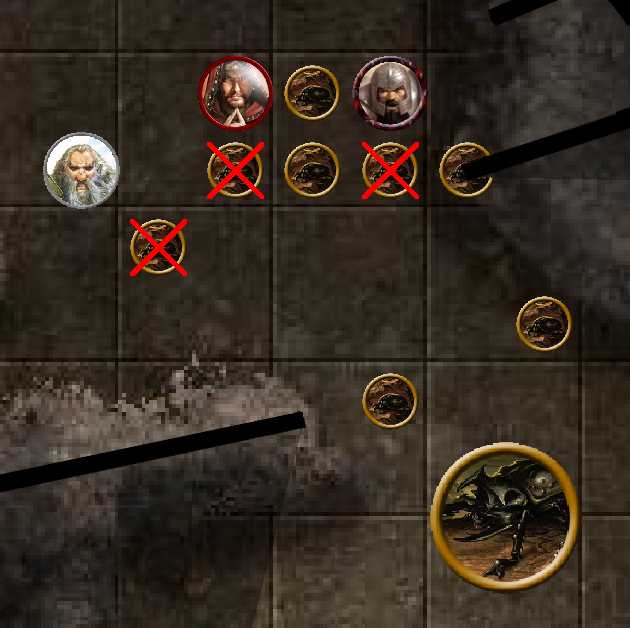
\includegraphics[width=0.7\linewidth]{./figs/playthrough/bug-fight.png}
\vspace{0.5 cm}
\end{center}

The powerful mandibles rip his shield from his arm, severely weakening his defences. Maras manages to sling a powerful Black Bolt on the monster incurring significant damage. Over the next few rounds the huge monster bug misses several consecutive attacks on Nostromo, giving Maras and Datarian time enough to land a barrage of strikes, killing it. After that it is just a matter of a few more rounds to clean up the rest of the smaller black bugs.

Just beyond the slaughter site they find the way out of the cave system, and an hour later emerge out on the side of the mountain, a couple of leagues from Eisenkrafs. They now make their way back to Sleepy Cove, and get attacked by the most pitiful bandits one night. Seems bandits are common around the northern road.

In Sleepy Cove they give the GreenStone to Dyslexia Marigt and get their reward before taking a day to rest and shop. Next up is the Tower of Ho-Bliz Wayze, to persuade him to sell the BlueStone.


\subsubsection*{Session 11: Is the BlueStone perchance for sale?}
% originally posted 100324
The heroic trio: Mandak, Anomali, and Datarian start the day with some light shopping, before setting out towards the Dark Tower of Ho-Bliz Wayze. The trip is uneventful and takes about three days.
When they reach the tower they see a fast hooded figure fighting with a white haired wizard. The colourful lights and strange sounds of Fireballs and Shock Fields fill the battle ground.

\begin{center}
\vspace{0.5 cm}
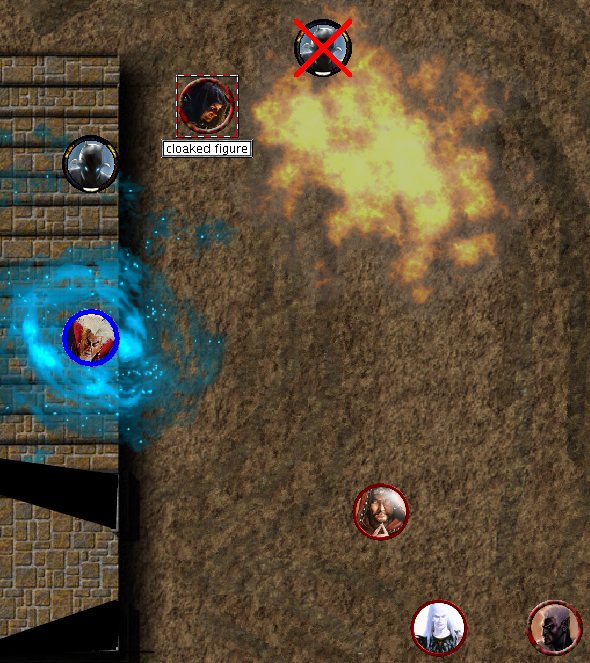
\includegraphics[width=0.7\linewidth]{./figs/playthrough/tower-fight.png}
\vspace{0.5 cm}
\end{center}

The hooded man wounds the white haired wizard and disappears into the tower. The Heroes pursue. Ten rounds of fast combat takes them into the tower in pursuit of The Hood, and make them realise that he is both very fast and very competent, and that he seems to have no intentions of killing them. He is here for something else.

They step back to the stairs and try to help the white haired wizard, but he dies from his wounds, gurgling blood and curses:
\begin{readoutloud}
Sneexious, that greedy idiot, she will never have the stone!
\end{readoutloud}
Then he promptly dies, and the heroes are left to fight their way through waves of the wizard's shadow servants as they search through the tower. At each level of the tower they find the hooded man, quickly going through the wizards things, searching for something. But, as fast as they show up, he continues up to the next floor. At the top he quickly jumps through a window and escapes.

When they have fought the last of the strange shadow servants in the tower they start a methodical top down search of the place. They find many valuable objects and strange artefacts, as well as the BlueStone. It was hidden away in a corner of a drawer, buried under old notes, together with a yellowing notebook of significant antiquity. Unfortunately they cannot read, yet, awaiting more xp to train the necessary skills...


\subsubsection*{Session 12: Looting the Wizard's Tower. What could Possibly Go Wrong?}
% originally posted 100404
Maras Blackhammer and Nostromo join the fray early in the session but Nostromo encounters a dinner emergency and has to disappear almost immediately. Datarian Blood takes up arms instead.

All the riches of the wizard's tower seems to be theirs for the taking. The question is what to take, since they have a shortage of bags. They take an old worn Banor's Gate at least, and Maras runs through the tower selecting the most valuable stuff he can find to cram down the already bulging loot sacks. Unfortunately he is a bit careless in his searching for riches, and suddenly he has awoken a small horde of shadow servants, emerging from the wall in a dusty storage room.

Maras and Datarian fight for their very lives through some 50 rounds of intense close quarter combat and ridiculous kiting and re-grouping actions. After much hassle, pain, and bloodshed, they finally manages to diminish the overwhelming numbers and devise a working strategy to destroy the last remaining shadow servants.

After this they quickly grab their loot, check a few details in the tower, then get on the road back towards Sleepy Cove.
On the way they stop for a day in Castle Conq village and sell their loot, shop some gear, and spend some xp, before continuing on towards their employer.

They enter Sleepy Cove late in the night, and immediately hand over the BlueStone to Dyslexia Marigt who is ever so grateful. She pays the reward, but they almost forget about the double pay for all three stones. Dyslexia doesn't have all the money here yet. She has sent for more funds from Trade Town, but the boat is a few days late. She'll have their gold soon though, as soon as the boat arrives.

They decide to stay in Sleepy Cove until they get paid. But memory is short and distractions are many.


\subsubsection*{Sessions 13-14: Revenge in Eisenkrafs}
% originally posted 100409
Nostromo and Datarian Blood sit in the "Sleep with the Fishes" inn, drinking beer, when Sam Slick walks in. Datarian recognises him as the hooded figure from the Wizard's Tower. Sam and Datarian exchange some acidic but slightly friendly remarks about towers, loot, and life in general. Sam offers to sell the Heroes some important information for 5 gold. Datarian declines.
Sam Slick then goes to talk to Singalot the Bard for a while. Passing Bling SwordSlash, he gives a disapproving nod. Bling looks disgusted as he nods back. It is evident that they don't like each other much at all.

Bling is a bit and tipsy sidles up to Datarian. He says: "I wouldn't trust Slick", and some further remarks about inferior morality, unheroic attitude, etc. Then he goes back to his harem of willing young village women.
Sam gets up to leave, but before he goes out the door he says to the Heroes: "5 gold, might save your life." He also tells them that Bling SwordSlash's "high moral values" tends to kill more people than they save. Then he leaves into the night.

The next day Datarian and Nostromo decide to take revenge on Goebbels and the other villains in Eisenkrafs. They pack their provisions and set out north for a few days' travel. They reach the horrible little mining village and proceed to march into the mining yard office. There is Gebbhard Goebbels, who is not too pleased at seeing the Heroes alive and well. They summarily chop him in two before help can arrive, but not before he sounds the alarm. Soon enough several ruffians come charging at the office from two fronts.

A lot of killing and maiming ensues. They manage to kill off half the ruffians before the rest flee. Then they loot the office, finding a few silver. But! Datarian has the bright idea to break into Goebbels' house to search for more loot.

In Goebbels' house they find a lot of lootable items at reasonable value density, and they also find a trap door leading down into an old basement. The sublevel turns out to be more of a tomb than a basement, and it's very, very, old. The architecture looks similar to the old altars they found in the natural caves below mine shaft 5-1. They start to get a \emph{baaad} feeling about this.
Nostromo the Blind immediately steps into a trap, and two ghostly sentinel warriors appear on either side of him.

\begin{center}
\vspace{0.5 cm}
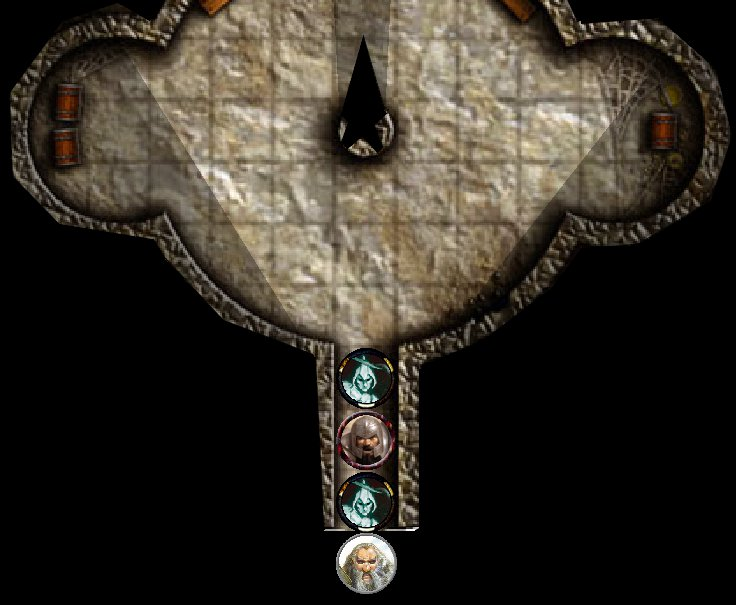
\includegraphics[width=0.7\linewidth]{./figs/playthrough/goebbels-basement.jpg}
\vspace{0.5 cm}
\end{center}

Their immaterial swords slice through his shield and armour inflicting wounds as they go, and they don't seem to take any damage from his mighty axe. Maras Blackhammer quickly climbs down to assist his friend.
The Black Bolt magic that Maras throws at the ghost sentinels seem to have the desired effect though, and one of the ghosts disappears as he is struck. The other ghost strikes Nostromo a couple of times more before it bows and disappears.
Looking around they find some old chests in the alcoves and a large sarcophagus. They loot the chests for money, sealed sentinel stone discs, and a master crafted sword. They leave the ominous sarcophagus alone.

Then they move out into the village in search of a donkey to carry all the loot. However, lots of miners have gathered around the house to stop them. They fight a loosing battle for a while until they have managed to kill off all the ruffian leaders. Then Datarian manages to calm the rest of the crowd down, and they agree to stop fighting.
In the end the people of the village sells them an old donkey, and allow them safe passage if they go quickly and don't come back.

But \emph{quickly} seems to be a problematic word, and the Heroes take a trip back down the basement again to pry open the sealed sarcophagus. And they wake a horribly powerful old mummy. Nostromo immediately flees, screaming like a little girl. He is soon joined by Datarian and Maras as the mummy's shrieking roar rises to a fearsome battle cry.


\subsubsection*{Session 15: Help! What Do We Do with an Angry Mummy?!}
% originally posted 100414
Datarian Blood and Maras Blackhammer stand in Goebbels' house, around a large heap of furniture. Nostromo is away tinkering with his car, and this gives the Heroes pause. They debate forever over how to proceed. Below all the furniture is the trap door that leads to the basement ... and the Angry Mummy!
Should they go down there just the two of them, or should they try to raise more manpower? In the end they decide to try recruiting from the village. Datarian puts on his most charismatic smile and goes out the door to speak with the ad hoc leader of the village mob, Jerker.

Jerker is a bit annoyed that they are still in the village. He wants them gone and out of Eisenkrafs. They have proven to be very violent, and obviously untrustworthy since they refuse to leave the house of their vanquished foe despite getting a donkey. However, Datarian is a smooth talker and slowly convinces him that they really must stay a little longer, for the good of the village. Seeing as there is a Mummy on the loose in Goebbels' basement, and a Rampaging Mummy is really bad for the already abysmal real estate value of the village.

Maras has taken the time to read some of the papers they have found, and has figured out that Goebbels was organising a complex scheme of theft, embezzlement, and betrayal between several parties. He seems to be in league with a group of merchants to swindle the village and Baron Conq out of a significant fraction of the mine's production output. He also betrays the merchants by giving freight information to a local bandit gang, and he thus manage to also sell mediation and protection services to other merchants and travelling parties. All in all a rather convoluted, and sinister tangle.
Maras explains a bit of this to Jerker, and gives him the evidence. Jerker has already sent a messenger to Castle Conq asking for the Baron and a Law man to tell them what to do about the murder of Goebbels, and the future management of the village.

Since it seems that Goebbels was much worse than everyone already knew, Jerker becomes more accommodating to the Heroes. He says there are two solid orc fighters in the village. They are in the mine at the moment, but he'll get them to stop by Goebbels' house when they come out of the mine. Jerker is also asking about the money Goebbels must have stowed away from his scheming, but the Trustworthy Heroes explain that they have found nothing much in the way of money or valuables yet.
Finally Jerker tells them they can stay the night in the village to fight the Mummy tomorrow, but he will have the village mob standing by outside the house if they try any more untoward violence.

Later that evening the orcs Grishnach and Merchar knock down the door and present themselves for Mummy fighting detail. They want 5 silver each to fight, and they do look imposing. Datarian and Maras agree, and the orcs should return in the morning. After that the Heroes try to sleep for the night but are constantly interrupted. Repeated icy screams from the basement and rattling furniture on top of the trap door does not make for a good night's sleep.

They wake in the morning, bleary eyed and tired. The orcs have armed themselves just fine, and are ready to protect their village and make a lot of money in the process.

They open the trap door and look down, ... clear. They quickly climb down, and spread out in a very organised attack pattern. Of course the Mummy just emits one of his horrible fearsome screams and everyone but Maras quickly disappear up the ladder in panic.

Fighting the Mummy is problematic. They spend some 30 rounds and several attempts followed by scared to death panicked flight up the ladder, then gathering and climbing down again to try anew. Datarian is close to death at one point, but in the end they prevail against the Undead Horror. They take the loot and pay the orcs another 5 silver each as a bonus.

Afterwards they pack their second hand donkey and leave Eisenkrafs, hopefully for good this time. Early the next day, in the foot hills of the mountains, they feel something is wrong, but cannot quite put their finger on it... There is trouble afoot...


\subsubsection*{Session 16: Why are there Always Bandits on this road?}
% originally posted 100421
Since the Heroic few dawdled in Eisenkrafs for sooo long, it was a simple task for the Eisenkrafs Bandits to track them down when they left, and set up an ambush.
The Bandit Boss, two axe men, and two archers attack Datarian and Maras as they lead their loot laden donkey southward.

The battle is fierce and difficult. For 13 rounds they fight for their very lives. In the end the heroes prevail, seriously bloodied and wounded. They have slain the boss and one of the axe men, and taken the other prisoner. The archers managed to flee.

The good natured Heroes gladly torture their prisoner. Under significant blood letting, leaving him at the brink of death, he tells them about the hidden bandit camp about an hour or two south east of Eisenkrafs. He also explains the deal they had with Goebbels, where he would tell the bandits of all coming and going shipments, numbers, guards, etc, then split the loot 50/50.


\subsubsection*{Session 17: Where is The Old Lady? She Owes Us Money!}
% originally posted 100429
\begin{readoutloud}
The Heroic band get sidetracked from their bandit hunt by the GM's lack of memory. Since the GM has simply forgotten to finish the Eisenkrafs Bandit Camp the heroes instead take a side interest in the main quest arc again.\\
\emph{-- Yep, that really happened!}
\end{readoutloud}

After thoroughly questioning the captured bandit, to the brink of death, Datarian Blood and Maras Blackhammer travel via Castle Conq to drop him off for proper justice to be served, and get a small reward. Then they continue to sell loot from their Eisenkrafs Revenge Expedition, before finally going back to Sleepy Cove.

In the "Sleep with the Fishes" they meet Farsalos, a curious rookie, who they drag with them for their next adventure. They stash some loot in their room and then go to visit Dyslexia Marigt, only to find out that she is no longer in her cabin. Many of her belongings are also gone. They ask the neighbours who tell them that she left earlier in the day towards the east. She had waited for the heroes for quite some time, then finally given up and left.

Back at the inn the generous Maras happily offers John AllBeard five coppers a day to help them track down Dyslexia Marigt. He accepts and they are all ready to travel, when all of a sudden the door bursts open. Farmer SmallBeard runs in and shouts "Where's my daughter? Has anyone seen her? She is gone!". Bling SwordSlash offers to help him find her for 20 gold, but the poor farmer has nowhere near that even if he sells the clothes on his back. The Generous Heroes however are happy to help him for all they coin he has and the promise of an old donkey.

Farmer SmallBeard explains that he heard a scream from the barn, and when he went out to look he saw a large red cloaked man disappear into the forest with a large bundle over his shoulder. The man was too fast and disappeared into the woods, and must have kidnapped the beloved daughter.

Datarian Blood, Maras Blackhammer, and Farsalos the rookie load up on provisions, and together with John AllBeard set off towards the east in pursuit of Dyslexia Marigt, and just hope that it was her RedGuard who took the daughter.

They journey leads towards the old Ashen Lake bed. Which according to John AllBeard is a site of unspeakable evil, where once in antiquity a horrible monster was summoned to the ruin of all the lands.

Once there they hear chanting far away and sneak up through the pitiful woods towards a large altar platform. Dyslexia Marigt is there, performing some kind of ritual, a RedGuard is watching over her, and they can also hear the sobbing cries of the kidnapped girl.
As they advance the RedGuard notices them and tells them to stop. But they don't of course, and finally Dyslexia Marigt orders him to kill them, and proceeds with casting a "slow" spell on Datarian and Farsalos.

\begin{center}
\vspace{0.5 cm}
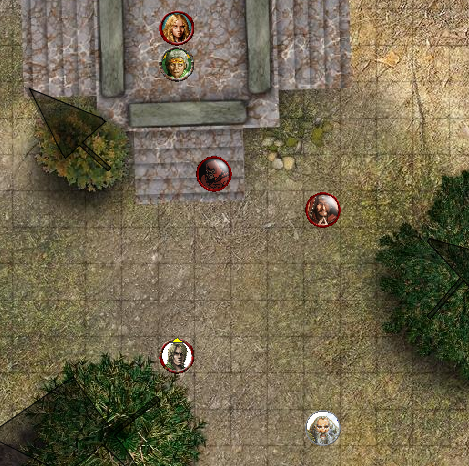
\includegraphics[width=0.7\linewidth]{./figs/playthrough/summoning-altar.png}
\vspace{0.5 cm}
\end{center}

The fight is very uneven as the fast RedGuard easily keeps the slowed Datarian and Farsalos at bay and even seems able to fight them off, despite Maras artillery support of heavy Black Bolt spells.

Then, suddenly, in the northern ash field an ominous boom is heard and a large cloud of black silt is thrown into the air. Farsalos is very scared and chooses to go to bed for the night.

\subsubsection*{So That's Uchly Namen? ... Fuuuuuuuck!}
% ... continued ...
Finally the Heroes manage to turn the tide, and the RedGuard goes on the defensive. But Dyslexia Marigt enters the fray and throws a massive Black Bolt at Maras. It is evident they have to change tactics. Suddenly they also hear a shout from the eastern cliff, and see Sam Slick appear, offering his services to the highest bidder. Dyslexia takes him on, but Datarian raises the bid.
Maras keep the RedGuard busy while Datarian charge the duplicitous old lady. Datarian quickly kills Dyslexia Marigt with a few mighty sword strikes, just in time to see an Enormous Green Monster with glowing eyes, fangs, and huge horns approach from the northern ash fields, emerging from the dark cloud.

Maras ignores the RedGuard and dash towards the altar to help save the girl. Sam Slick flees with a comment about that beast costing far more than the 15 gold he was offered. The RedGuard quickly flees as well now that Dyslexia Marigt is dead and the beast approaches, but not before he runs past her corpse and snatches something to take with him.

\begin{center}
\vspace{0.5 cm}
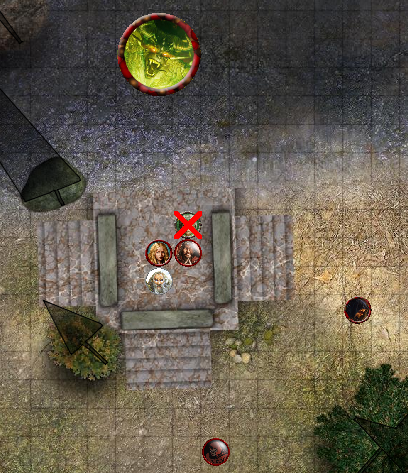
\includegraphics[width=0.7\linewidth]{./figs/playthrough/summoning-demon.png}
\vspace{0.5 cm}
\end{center}

They manage to free the girl and run away as fast as they can, with the demon in a half hearted pursuit.

Back with John AllBeard they immediately start tracking down the fleeing RedGuard, and follow him for the rest of the day and a bit into the night. Finally, in pitch black, they come upon the Old Eastern Tower Ruins.


\subsubsection*{Session 18: Devious Meetings in the Dead of Night}
% originally posted 100501
Datarian Blood and Maras Blackhammer got bitten by the gaming bug and ordered up an extra session. So, in the dead of night they sneak through the deep forest towards the Old Eastern Tower Ruin, following the wounded RedGuard. Well, I say sneak, but in truth none of them can sneak, so they get noticed very quickly.

They manage to see the RedGuard talking with a grey haired, pale, thin man. Then the RedGuard finds them and sounds the alarm. They engage the RedGuard and the grey haired man just outside the entrance to the ruin. The RedGuard immediately shoves the man into the ruins and shouts "Trymore, protect the Baron!", then he engages the Heroic Duo.

Datarian and Maras hold their own for a short while against the RedGuard, but when two more RedGuards quickly emerge to join the fight the outlook is bleak indeed. The Heroes fight for a few more rounds before making a controlled retreat.

They rest for the night to regain strength. Then, in the morning, they send in John AllBeard to scout the terrain. He returns quickly saying that the Baron and his guards disappeared west during the night, and the skinny man and one guard have travelled east on foot. The heroes immediately pursue Trymore and his RedGuard.

Late in the evening they intercept them, on a hill looking out over the Merna village and valley. They fight Trymore and his RedGuard by a dangerous exchange of Black Bolt spells. As Datarian manages to land a hard blow on Trymore he teleports away on the brink of death, bringing his RedGuard with him.
Datarian and Maras assume he has teleported back to the eastern tower ruins.

They decide to rest for the night and make camp on the hill. As the sun sets they see the huge lumbering shape of Uchly Namen in the distance, moving north towards the village.
As the monster reaches Merna he starts razing houses and eating things, spreading chaos and destruction in his wake. Some 15 minutes later he marches on towards the north east, and the terrified townsfolk can return to try to put out the fires of the last few houses still standing.

The next day the Heroes travel back to the Old Eastern Tower Ruins, where they find Trymore and the RedGuard. After a very difficult fight, where they are balancing on the edge of death they manage to kill Trymore and take the RedGuard captive.
The RedGuard has yielded and offers up some information on the horrible plot. In essence: Baron Conq has hired both Sneexious (Dyslexia Marigt) and Trymore John to raise the demon Uchly Namen to attack baron Pawa. Evilnius Conq seems to think the old ideas are the best, since he obviously tries a two hundred year old trick devised and attempted before by his ancestor.

The two Heroes now have the necklace Dyslexia Marigt built with the three stones they gathered for her. The RedGuard thinks it has something to do with controlling the Demon. Too bad they killed Trymore John, as he might have known more about it...

\

\emph{Note: at this point the necklace doesn't matter that much. The Demon has already been commanded to kill Baron Pawa and his Captain, and the necklace has lost most of the protective magic since no one has been maintaining it.}


\subsubsection*{Session 19: Castle Pawa has Fallen, and more Demons}
% originally posted 100505
The new Hero Wannabe, Farsalos, joins Maras Blackhammer and Datarian Blood in the Old Eastern Tower Ruins. Then they camp there for the night before setting out towards Castle Pawa in the morning. By the day's end they have reached the ruined village of Merna, where the townsfolk are slowly starting to rebuild. They generously spend way too much silver purchasing a map of the region and a new bow for Farsalos.

A couple of days later they reach Castle Pawa, and see from afar the thick black smoke rising from the town. When they enter the town they see the broken battlements, the large pools of blood still colouring the ground, the smoking ruins of many of the buildings. Wounded soldiers and hollow eyed townsfolk stand around talking about the horrors of the previous night's attack.

\begin{center}
\vspace{0.5 cm}
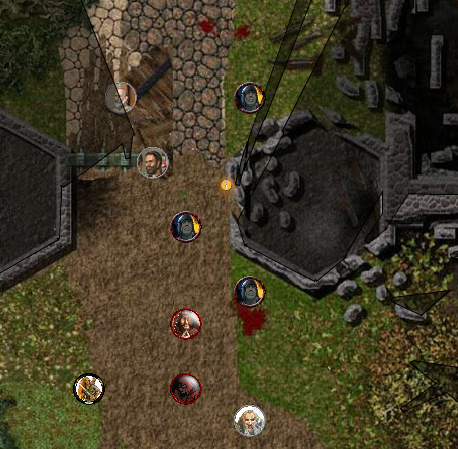
\includegraphics[width=0.7\linewidth]{./figs/playthrough/castle-pawa.png}
\vspace{0.5 cm}
\end{center}

They continue through the ruined city, gathering tales of the horrible demon's destructive prowess. Uchly Namen went through the city in a few hours, picking up people and screaming at them in long complex battle cries before tossing them away or eating their heads.
In the end he smashed through the strong defensive tower where Baron Pawa and his wife were hiding, and killed them both. Then he rested for a bit on the ruins of the northern gate, before heading out and away.

The Heroes meet the Captain of the Guard and get a more consistent tale of the previous night's events. The Captain says they hit the demon several times with siege weapons, and managed to give it some serious wounds, but normal weapons were almost useless. The Captain seems to think the Baron was the target of the attack. The monster seemed to be looking for something for most of the time it was wrecking the city.
The captured RedGuard tells his tale and it is clear that Baron Conq wants to strike at the Pawa family.

Maras convinces the Captain that they are demon hunters, tracking Uchly Namen to slay him, and that there is a spear and shield stored somewhere in the castle. Magical weapons created to fight the Demon. Since Maras haven't been able to decipher more than a little bit of Honorbliz' BlueStone journal he asks the well educated Captain to read more.
They manage to figure out that it was during the reign of Massa Pawa, some 200 years ago, that the spear and shield were returned to the keep. The Captain knows which of the many heirloom weapons they mean.
He leads them to the foyer of the main keep and take down a strange looking greenish lance spear and a similarly odd tall narrow shield. Upon the Word of their Honour Maras Blackhammer is allowed to borrow the weapons to slay the Demon Uchly Namen, then return them. The captain also says that the new Baron in absence, Heirling Pawa, will probably reward them when he returns from his long travels.

The Heroes rest for the night, then set out the next day towards Honorbliz' tower to search for a ritual to close the gate forever. On the way they get ambushed by a pack of Grey Stalkers. The fight is vicious, with the odd reality blinking of the demonic foes giving Datarian great trouble in slaying them. Maras and Farsalos do significant damage with their ranged weapons though.

\begin{center}
\vspace{0.5 cm}
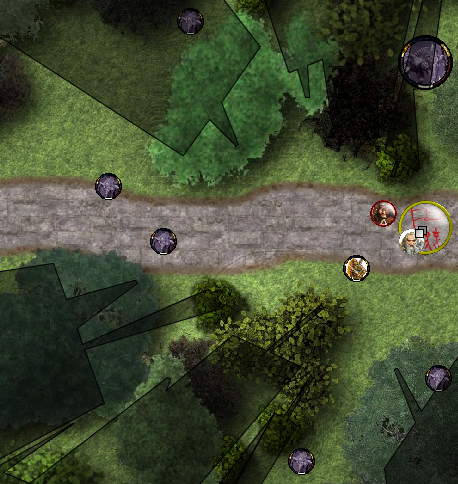
\includegraphics[width=0.7\linewidth]{./figs/playthrough/grey-stalkers.png}
\vspace{0.5 cm}
\end{center}

In the end, after 14 rounds of frenzied combat they manage to slay all but one of the stalkers. Farsalos is nearly dead, Maras is almost out of mana, and Datarian is pissed off. The last stalker runs away, fast, into the forest and disappears.


\subsubsection*{Session 20: Return to the Tower, Lawyers on the Loose}
% originally posted 100517
They continue their journey towards Honorbliz Wize's tower. As they arrive they see the tower grounds are cordoned off with miles of red tape, and wagons full of travelling lawyers have put the area under siege. They walk up to one of the bald men, representing the firm of Wasterich, Goldburn, Takesilver, and Sidethorn, and ask him about what is going on. The well dressed legal representative responds by a lengthy tirade of strange words, slowly conveying the fact that the wizard, being hundreds of years old, had many, many, and even more children, most of whom are now fighting over the inheritance. However, the assembled army of lawyers have run into a problem with the wizard's servants. The strange shadowy creatures don't respect the letter of the law and have already killed two aggressive litigators. They have sent for a wizard to help them, but in the mean time they are waiting, and billing their clients of course.

Datarian and Maras quickly suggest that they will clean out the problem for a mere five gold. Farsalos is still newbie enough to gladly agree without further thought to the problem.
During the evening the Heroic trio hack their way through the hordes of shadow servants that have infested the -- now very clean -- wizard's tower. After a lengthy but boring battle they finally manage to barricade the closet from which the servants spew forth. Then sit down to go through the old journals stored in the many book shelves, looking for the gate closing ritual mentioned in the old book they found with the BlueStone. At the break of dawn, after much red-eyed and murderously slow reading, Datarian manage to pick the correct journal from a shelf, and they can leave this horribly tidy place.
But of course they manage to stuff their back packs a bit with some extra loot before they leave.
The lawyers pay them for a job well done, and when asked about news of the Demon Uchly Namen reports that a monster has been sighted moving around in the forest, towards Sleepy Cove.

The next few days the Heroes travel towards Sleepy Cove, via the market place at Castle Conq where they sell some loot.

In Sleepy Cove the situation is tense. Sightings of a large monster have been made in the vicinity, and the beast is heading towards the village. "It could be here any day" says one of the hunters.
And, as on cue, the beast wanders into the outskirts of town, following the main road towards the harbour.

The villagers call for a Hero to come forth and slay the beast, but since Bling SwordSlash demands 200 gold for the job they simply can't afford him. The Heroic trio of Datarian, Maras, and Farsalos ask for 50 gold and the villagers counter with something around 20+, whatever they can find in their meagre savings.
Datarian takes up the Spear lance and Shield, and feel the weapons awakening as the Dread Demon closed in.

With cautious panic they engage the Ancient Evil. Bling stand to the side, offering a few helpful and acidic remarks on how it should be done, and Datarian flying through the air back and forth as the Demon lands devastating blows on the shield.
It is obvious that the monster is hurt from the enormous battle of Castle Pawa, and Datarian manage to land a lance thrust with the spear which cuts a deep hole in the side of the demon. Then he get swatted away, again, sailing a dozen metres through the air before striking the ground just behind Bling, who supplies a helpful \emph{"That's not the way to slay a demon".}

\begin{center}
\vspace{0.5 cm}
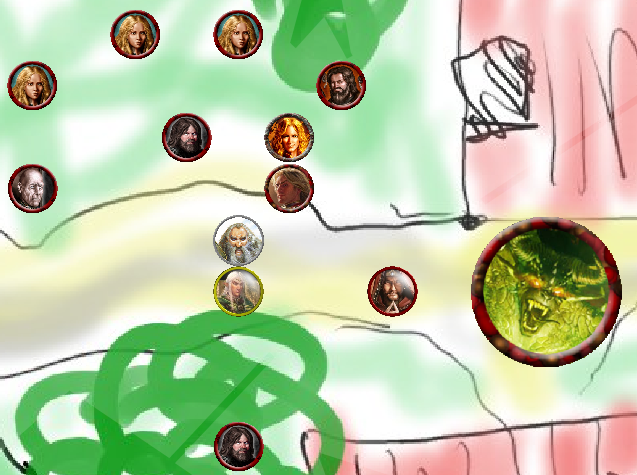
\includegraphics[width=0.7\linewidth]{./figs/playthrough/battle-sleepy-cove.png}
\vspace{0.5 cm}
\end{center}


\subsubsection*{Session 21: The Showdown: Fighting Uchly Namen}
% originally posted 100518
Farsalos, Maras Blackhammer, and Datarian Blood continue their lethal battle against the Horrible Demon Uchly Namen. They have retreated continually along the main street of Sleepy Cove as the Demon advances. Datarian has spent more time in the air than on the ground, and is feeling the effect of the many heavy blows from the mighty fists of the monster, despite the protection of the magical shield.

The battle rages on, until Maras digs through their pack bags on the donkey, fishing out the necklace with the three stones they retrieved. Uchly Namen quickly zeroes in on Maras and starts chasing him through the village, running down trees and outhouses as he steams by like a lumbering out of control locomotive. Just before the Demon is able to reach Maras and stomp him into a wet puddle Maras manages to pass the necklace onto Farsalos in a relay switch worthy of a professional athlete. Farsalos puts the long legs ahead and runs out of the village, kiting the furious Demon a few steps behind him.

They continue a bit south of the village, then it becomes evident that the demon will catch up with him sooner or later as Farsalos runs out of stamina. In a desperate attempt to avoid liquefaction Farsalos winds the necklace around an arrow and shoots it far out into the ocean. Uchly Namen stops, roars a long angry tired harangue of ancient foulness, then dives into the ocean to retrieve the jewellery. The Heroes retreat towards the village.

It takes some time before the monster appears again, walking out of the waves. He stops on the beach, Angry, wet, and wounded. Raising a fist he roars towards the village then stomps on to the east and disappears into a copse of trees.

The Heroic Three tells the relieved townspeople to have their 50 gold payment ready in five days, then bring John AllBeard along to track down the Demon.

Two days later they stand outside Castle Conq, where the Demon have razed a section of the wall before retreating. They talk with a few of the towns people and find out that the monster came out of the south forest, charged the castle wall and brought it down before retreating. The Conq guards had massive siege weapons ready and waiting when the monster appeared. Since the beast was already quite wounded he gave up quickly.

They follow the trail south down to the summoning site. There they find that the tracks vanish in the middle of the ashen lake bed. The Demon did not leave the spot, and must have vanished into thin air.

Maras wants to try to seal the gate with his new found ritual book, but after the last few days of studying it is evident he will need to increase his magic skills significantly before being able to do so. Or, they can try to hire another wizard to do the job for them. The major hurdle though is that the ritual requires the necklace... Did Uchly Namen bring that with him when he disappeared? After a fruitless day's searching they give up and return to the village to claim their reward.

A few days later they are resting at the Sleep with the Fishes inn. The poor townsfolk have gathered every last coin they have saved to pay the 50 gold reward. The starving children, the coming winter, etc, etc, do not deter the Benevolent Heroic Three from pocketing the money and spending a day or two at the inn.

Later on they have travelled to Castle Pawa, where they meet the Captain again and return the Lance Spear and the Narrow Shield. They have to be careful since Baron Evilnius Conq have installed himself as Ruler and Saviour until the next Pawa youngling can return to claim his birthright. The Captain says that he thinks Heirling Pawa is somewhere to the east, travelling the world. But that is another story...

\

%\emph{Note, edit 180208:} It would have been better to have had Baron Conq's men murder the Captain so that no trusted leader of the town would argue against his version of The Truth. But let's just assume the Captain was smart enough to keep quiet about what he knows regarding Baron Conq's role in the disaster. This way also opens for a nice future adventure where they have to help combat Baron Conq when Heirling Pawa is returning for his birthright. Or perhaps take blood money from Conq to disappear the young Heirling Pawa...


\subsubsection*{closing remarks}
% originally posted 100518
This brings an end to the Return of Uchly Namen.
The campaign, documents, maps, tokens, campaign files, etc, will be released on the gallery site later on. The full set of original files is also available, but is a fair bit larger, and will have to be uploaded somewhere else I think.

\

\emph{Note, 180208: The whole campaign was uploaded to the rptools user gallery, but that site quickly went down and disappeared, taking the files with it. I still have the originals. Hmm, will continue to clean out given time, and push the whole package somewhere.}

\

The adventures of Nostromo, Mandak, Datarian, Anomali, Maras, and Farsalos will continue ... in "Dark Klan".











%===============================================================================
\end{document}
